\pdfoutput=1

\documentclass[cits]{JINST}
\let\ifpdf\relax % Avoid clash between packages (\ifpdf)

\newcommand{\unit}[1]{\ensuremath{\mathrm{\,#1}}}
\renewcommand{\u}[1]{\unit{#1}}
\newcommand{\um}{\textmu m}
\DeclareFontFamily{U}{euc}{}
\DeclareFontShape{U}{euc}{m}{n}{<-6>eurm5<6-8>eurm7<8->eurm10}{}
\DeclareSymbolFont{AMSc}{U}{euc}{m}{n}
\DeclareMathSymbol{\umu}{\mathord}{AMSc}{"16}

\usepackage{caption}
\usepackage[pdftex]{graphicx}
\usepackage{amsmath}
\usepackage{afterpage}
\usepackage{wrapfig}
\usepackage{tabularx}
\usepackage{subfigure}
\usepackage{caption}
\usepackage{tabu}
\usepackage{booktabs}
\usepackage{multicol}
\newcommand{\comment}[1]{{\fontsize{10}{10}{\par \tt\textbf {\selectfont #1}} \par}}

\graphicspath{{figs/}}

\usepackage{lineno}
\linenumbers

\title{Separation of nearby hadronic showers in the CALICE SDHCAL prototype detector using ArborPFA}

\author{The CALICE Collaboration. Email : \href{mailto:rete@ipnl.in2p3.fr}{\tt rete@ipnl.in2p3.fr}}

\abstract 
{
A new reconstruction algorithm, ArborPFA, is being developed to separate nearby hadronic showers in the SDHCAL prototype. This intends to demonstrate the capability of high granularity hadronic calorimeters such as the SDHCAL to efficiently apply Particle Flow Algorithms. The reconstruction algorithm we present here uses the tree-like structure features of hadronic showers, that high granular calorimeters reveal, to associate hits belonging to each hadronic shower and to reduce confusions between two close-by showers. The results of these studies indicate a good single particle efficiency and reconstructed energy. A powerful separation down to distances of 5 cm is obtained.
}

\begin{document}

\keywords{Keywords: Particle flow; Calorimetry; ILC; SDHCAL}

\newpage
%%%%%%%%%%%%%%%%%%%%%%%%%%%%%%%%%%%%%%%%%%%
%%%%%%%%%%%%%%%%%%%%%%%%%%%%%%%%%%%%%%%%%%%
\section{Introduction}

~~~~~~~To study the Higgs boson properties and to extend the discovery of new particles beyond the scope of LHC, linear (e.g ILC or CLIC) and circular (e.g FCC or CEPC) e$^+$ e$^-$ colliders are proposed. An important requirement of such a machine is to provide a good jet energy resolution ($\Delta$E/E $\sim$3-4\%) in order to distinguish between Z and W$^{\pm}$ bosons as well as to study the Higgs boson properties.

The Particle Flow concept has been proposed to achieve the ILC benchmarks \cite{ilc-tdr}. This algorithm aims to individually reconstruct particles using the most appropriate sub-detector for the energy and momentum measurement. An implementation of the particle flow algorithm called PandoraPFA has been developed \cite{pandora-pfa} and successfully applied in ILD physics performance studies and to close-by hadronic showers separation in the CALICE SiWECal and AHCAL \cite{calice-pandora-paper}.

To apply efficiently the Particle Flow Algorithms, both good energy resolution and fine transverse and longitudinal segmentation should be provided by the \textit{electromagnetic calorimeter} (ECAL) and the \textit{hadronic calorimeter} (HCAL).

Different calorimeter technologies are currently under study by the CALICE collaboration to fulfill these requirements. In this framework, a \textit{semi digital hadronic calorimeter} prototype (SDHCAL) was built \cite{sdhcal-paper} and successfully tested at the CERN H6 test beam line of the SPS (CERN) in 2012. With a transverse readout segmentation of 1 cm$^2$, 48 sampling layers and good energy resolution \cite{sdhcal-paper}, this calorimeter statisfies ILC requirements. 

In this paper, we present another approach of the particle flow : the ArborPFA approach. The algorithm has been designed for high granularity calorimeters and applied to SDHCAL test beam data and Monte Carlo simulation samples. We evaluate the performance of the algorithm on single pion events and study the ability of the algorithm to separate two overlaid pion showers at different separation distances and energies.

%\newpage
%%%%%%%%%%%%%%%%%%%%%%%%%%%%%%%%%%%%%%%%%%%
%%%%%%%%%%%% SDHCAL PROTOTYPE %%%%%%%%%%%%% 
%%%%%%%%%%%%%%%%%%%%%%%%%%%%%%%%%%%%%%%%%%%
\section{The SDHCAL prototype}

%%%%%%%%%%%%%%%%%%%%%%%%%%%%%%%%%%%%%%%%%%%
%%%%%%%%%%%%%%%%%%%%%%%%%%%%%%%%%%%%%%%%%%%
\subsection{The technological prototype}

The SDHCAL prototype is a sampling calorimeter which consists of 48 layers alternating 20 mm steel absorbers and 6 mm gas resistive plate chamber (GRPC) with embedded electronics. The gas gap between the two electrodes of the GRPC is 1.2 mm. 9216 pads (96 x 96) of 1 cm$^2$ compose the readout of each chamber, leading to a total number of 442368 channels. Signals from particles crossing the gas gap are recorded on those pads in a 2-bits format corresponding to 3 thresholds on the induced charge. A complete description of the calorimeter setup and its features can be found in \cite{sdhcal-paper}. 

The test beam data used in this paper were taken at the CERN H6 beam line in 2012. The pion event selection is also performed according to the selection presented in \cite{sdhcal-paper}.

%%%%%%%%%%%%%%%%%%%%%%%%%%%%%%%%%%%%%%%%%%%
%%%%%%%%%%%%%%%%%%%%%%%%%%%%%%%%%%%%%%%%%%%
\subsection{The Geant4 simulation}

The SDHCAL prototype simulation is performed using the Geant4 simulation toolkit \cite{geant4}. The geometry of the detector is described precisely using material descriptions (composition, densities, etc ...) with their positions and exact sizes in space. The simulated physics in Geant4 is described by \emph{physics lists} simulating electromagnetic and hadronic processes. In this paper, pion showers with energies from 10 up to 80 GeV are simulated in the SDHCAL prototype geometry using the FTFP\_BERT\_HP and FTF\_BIC physics lists. The simulation program records the Geant4 steps within the GRPCs gas gaps with different pieces of information such as their deposited energy, timing information, entering and exiting positions in the gap.

The calorimeter hits digitization is forwarded to an external program called \emph{SimDigital} implemented in a Marlin \cite{marlin-lccd} processor as part of the ILCSOFT reconstruction chain \cite{ilcsoft}. The digitizer outputs the real digitized hits as recorded in test beam data and are used as input by the ArborFA reconstruction program. Multiplicity and efficiency effects are also included in the simulation in order to reflect the test beam data. A more detailed description of the simulation and the digitizer can be found in \cite{sdhcal-sim-digit}.

One should notice that a discrepancy with test beam data on the total number of hits of hadronic showers using different physics lists is observed. Indeed, the deviation of the number of hits with respect to test beam data is less than 5\% from 10 up to 40 GeV but starting from 50 GeV up to 80 GeV, this deviation increases up to 15\%. This can be explained by other discrepancies on topological variables such as the radial extent of hadronic showers which is underestimated by Geant4 physics lists. Among the physics lists used in this simulation, the FTF\_BIC one shows a better agreement with data regarding the radial extent as well as the total number of hits. The FTFP\_BERT\_HP physics lists shows satisfactory agreement with hadronic shower data obtained with different other detectors \cite{atlas-energy-res}. In the following, these two physics lists are used to study the reconstruction algorithm.

\subsection{Energy reconstruction}

The reconstructed energy of a single particle is computed as follows :

\begin{equation}
  E_{rec} = \alpha(N_{hit}) \cdot N_{1}
          + \beta(N_{hit}) \cdot N_{2}
          + \gamma(N_{hit}) \cdot N_{3}   
\end{equation}
where N$_1$, N$_2$ and N$_3$ are the number of hits between threshold 1 and 2, between 2 and 3, and above 3, N$_{hit}$ = N$_1$ + N$_2$ + N$_3$ and $\alpha$, $\beta$ and $\gamma$ are quadratic functions of the number of hits N$_{hit}$. The nine parameters of these functions are extracted from a $\chi^2$ minimization performed over all the hadronic events in the energy range [10, 80] GeV with steps of 10 GeV. Due to the discrepancy on the number of hits at high energy, this minimization was performed on test beam data and simulation data independently. The nine parameters obtained for both data types are summarized in table \ref{SDHCAL_ENERGY_MINIMIZATION_PARAMS}.
% \begin{equation}
%   \chi^2 = \sum\limits_{evt} \frac{(E_{beam} - E_{rec})^2}{E_{beam}}
% \end{equation}
\begin{center}  
  \begin{table}[!ht]
    \centering
    \begin{tabu}{ l | c | c | c }    
      
      ~ & $\alpha$ & $\beta$ & $\gamma$ \\
      \hline
      1 & 0.038531 &  4.2258e-05 & -7.5465e-09 \\
      2 & 0.078429 & -5.6943e-05 & -4.9592e-08 \\
      3 & 0.127212 &  4.5641e-05 &  1.4114e-08 \\
      
    \end{tabu} ~~
    \begin{tabu}{ l | c | c | c }    
      
      ~ & $\alpha$ & $\beta$ & $\gamma$ \\
      \hline
      1 & 0.02935 & 2.9639e-05 & -2.05123e-08 \\
      2 & 0.09259 & 1.1228e-05 & -2.01646e-09 \\
      3 & 0.16633 & 3.0865e-05 &  2.97939e-08 \\
      
    \end{tabu}    
    \caption{\label{SDHCAL_ENERGY_MINIMIZATION_PARAMS} The nine energy parameters extracted from the $\chi^2$ minimization for test beam data (left) and simulation data (right)}
  \end{table}
\end{center}

%\newpage
%%%%%%%%%%%%%%%%%%%%%%%%%%%%%%%%%%%%%%%%%%%
%%%%%%%%%%%%%%%% ARBORPFA %%%%%%%%%%%%%%%%%
%%%%%%%%%%%%%%%%%%%%%%%%%%%%%%%%%%%%%%%%%%%
\section{The SDHCAL Arbor particle flow algorithm}

%%%%%%%%%%%%%%%%%%%%%%%%%%%%%%%%%%%%%%%%%%%
%%%%%%%%%%%%%%%%%%%%%%%%%%%%%%%%%%%%%%%%%%%
\subsection{Principle}

~~~~~~~The Arbor approach has been developed by Henri Videau for the ALEPH collaboration and was recently adapted \cite{arbor-manqi} for the ILD detector design. It is based on the idea that the hadronic shower development follows a tree-like topology.

Figure \ref{ARBOR_STRUCTURE} shows an example of a shower development (left) where all main components of the shower are present : charged particles, neutral particles, electromagnetic and hadronic components.
The same figure shows on the right a sampling calorimeter view of a shower interaction as seen in a highly granular calorimeter. The black arrows drawn on this view suggest the tree-like topology development of the shower.

With such an approach, the shower reconstruction follows a principle close to the underlying physics.

\begin{figure}[!ht]
  \begin{center}
    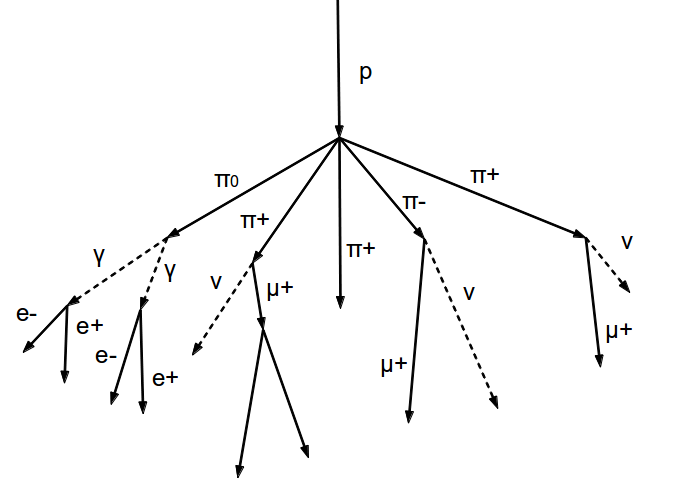
\includegraphics[width=0.45\linewidth]{ProtonDecay.png} \hfill
    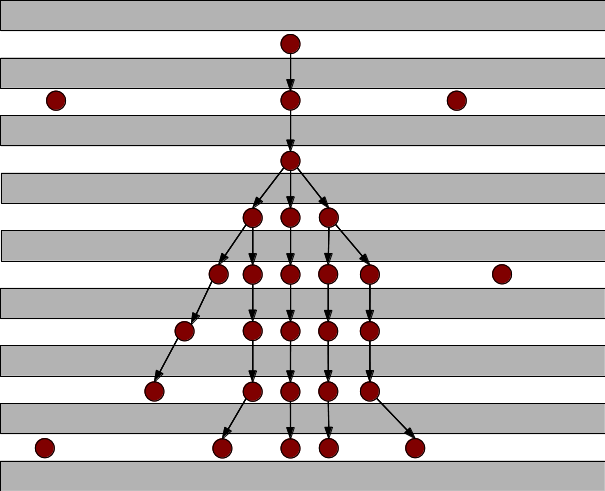
\includegraphics[width=0.45\linewidth]{ArborSchema.png}
  \end{center}
  \caption{\label{ARBOR_STRUCTURE} Left : schematic view of an induced proton shower. Right : schematic view of a reconstructed shower in a calorimeter with calorimeter hits (red).}
\end{figure}

The algorithm we use here is implemented using the PandoraSDK API, a toolkit for generic PFA development \cite{pandora-sdk}. The API is used in a Marlin \cite{marlin-lccd}  processor as part of the reconstruction chain in ILCSOFT \cite{ilcsoft} that produces reconstructed particle flow objects (PFOs). 

%%%%%%%%%%%%%%%%%%%%%%%%%%%%%%%%%%%%%%%%%%%
%%%%%%%%%%%%%%%%%%%%%%%%%%%%%%%%%%%%%%%%%%%
\subsection{Algorithms description}

The main goal of the algorithm is to create a set of clusters of hits representing a single particle. To cluster hits together, we proceed in three steps : a pre-clustering phase, a clustering phase and an association phase.

\begin{itemize}
  \item[\textbullet] Pre-clustering phase : Hits are grouped within layers using a nearest neighbour algorithm. If a group of hits contains 4 or less hits, it defines an \emph{object} to cluster during the clustering phase, otherwise the group is split up and each individual hit defines a separate \emph{object}. 
  
  \item[\textbullet] Clustering phase : the goal of this step is to connect previously created \emph{objects} in an oriented-tree-like topology. To achieve this, connections are created between \emph{objects}. Each \emph{object} is connected with other ones in the $N_{layers}$ next layers within a maximum distance $\Delta_{max}$. \\
  To obtain a tree-like topology, a cleaning procedure is needed for each \emph{object} in order to keep at least one connection in its previous layers. For each \emph{object}, a reference direction\footnote{The reference direction indicates the most probable direction for the connection to keep} is computed using the connection directions made in the next and previous layers. An order parameter\footnote{The order parameter quantifies the alignment with the reference direction} is defined for each object in the previous layers using the angle with the reference direction and the distance between the two \emph{objects} :
  
  \begin{equation}
  \kappa~=~\Big(\frac{\theta}{\pi}\Big)^{p_{\theta}} . ~\Big(\frac{\Delta}{\Delta_{max}}\Big)^{p_{\Delta}} 
  \end{equation}

  where $p_{\theta}$ and $p_{\Delta}$ are input parameters. The connection with the smallest order parameter is kept and other connections in the previous layers are removed. \\
  A second step of connection and cleaning is performed to align connections within hadronic showers using similar topological variables. Trees are finally created from the set of connected \emph{objects}.
  
  \item[\textbullet] Association phase : Trees are associated with each others to form reconstructed particle flow objects (PFOs).
  \begin{itemize}
    \item \emph{Track association} : Tracks are associated to tree structures that start in the $N_{layers}$ first layers at a maximum distance of $\Delta_{track-cluster}$ from the track projection to the calorimeter front face. 
    \item \emph{Neutral tree merging} Trees with nearby seeds\footnote{A seed is the unique \emph{object} in a tree that has no connections in previous layers} within the same layer are merged. This is necessary for interactions of neutral particles when the shower starting point is not determined by a single seed.
    \item \emph{Pointing cluster association} : Neutral fragments are merged in other charged or neutral fragments using cluster topological pieces of information such as the axis angle  compatibility. In case where a neutral fragment is merged in a charged fragment, the compatibility between the total energy and the track momentum is checked.
    \item \emph{Small fragment merging} : Remaining neutral fragments with a small size (less than $N_{obj}$) are split and each separate \emph{object} is merged in the closest tree, either charged or neutral.
  \end{itemize}
\end{itemize}

After all of these steps, particle flow objects are built from the produced clusters, one cluster per PFO. A PFO is considered as \emph{charged} when its cluster has an associated track, while a neutral PFO doesn't have.

A full description of the algorithm for the SDHCAL detector is given in \cite{arborpfa-can}.

%%%%%%%%%%%%%%%%%%%%%%%%%%%%%%%%%%%
%%%%%% Single particle study %%%%%%
%%%%%%%%%%%%%%%%%%%%%%%%%%%%%%%%%%%
\newpage
\section{Single particle study}
\label{SINGLE_PARTICLE_STUDY_SECTION}

%%%%%%%%%%%%%%%%%%%%%%%%%%%%%%%%%%%%%%%%%%%
%%%%%%%%%%%%%%%%%%%%%%%%%%%%%%%%%%%%%%%%%%%
\subsection{Setup}

\begin{wrapfigure}{r}{0.45\textwidth}
  \vspace{-20pt}
  \begin{center}
    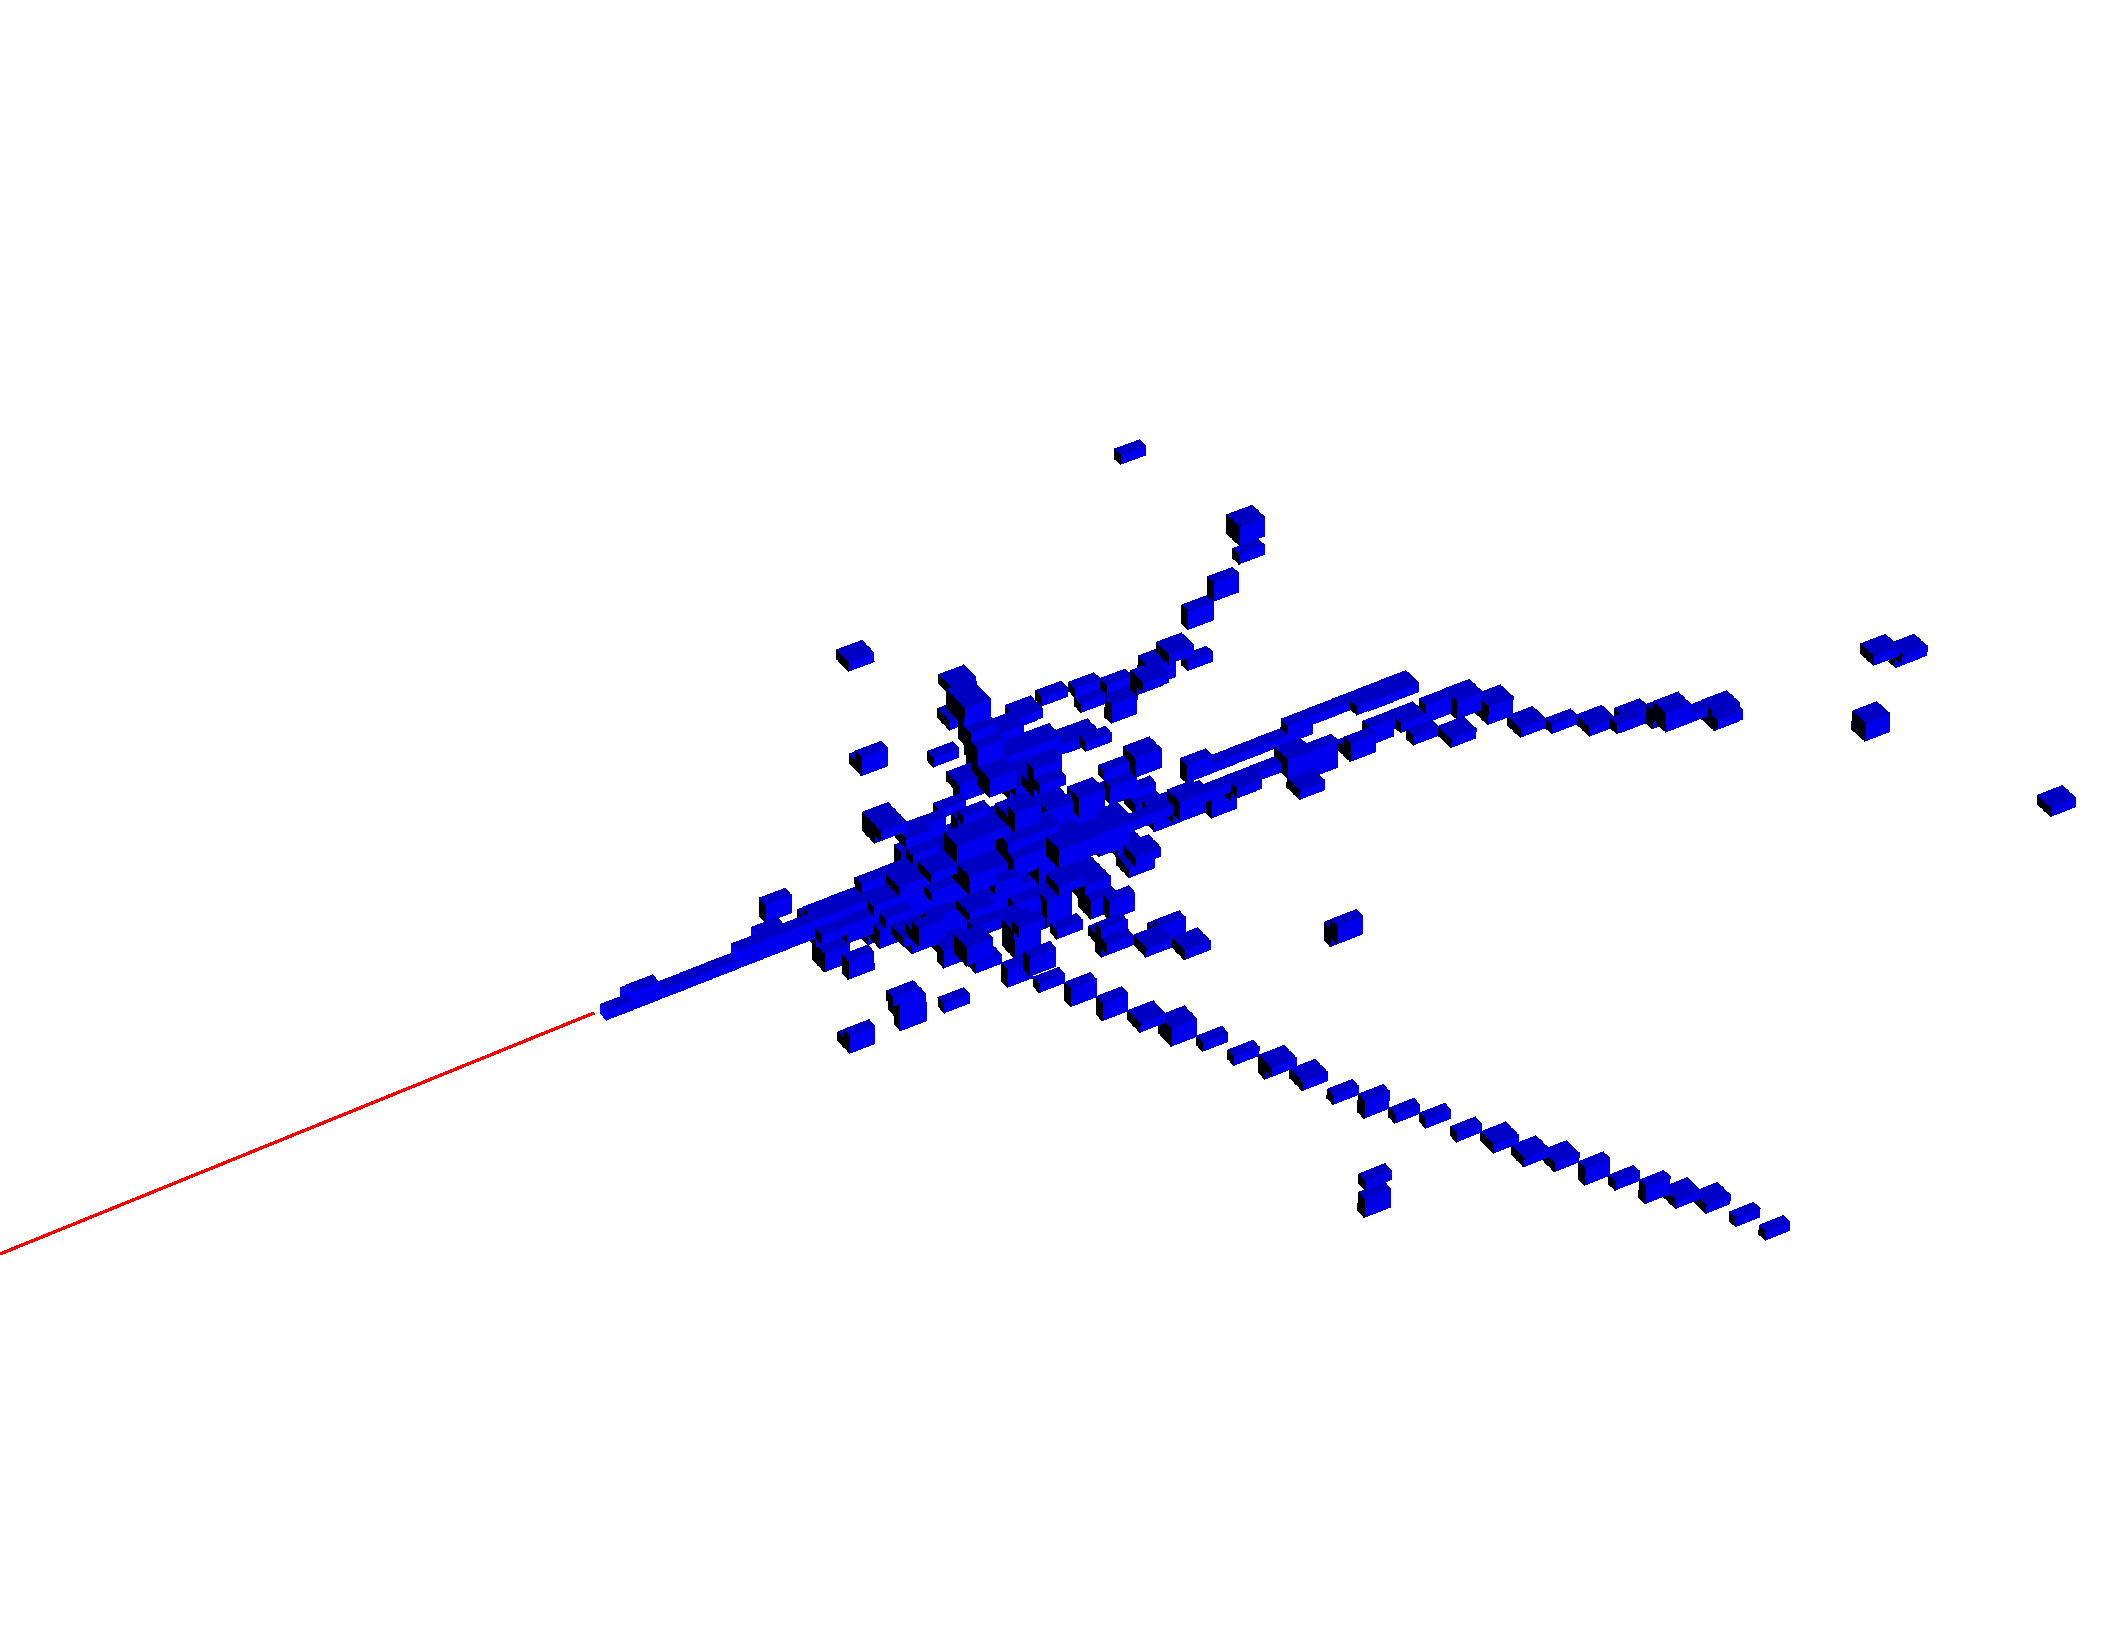
\includegraphics[width=\linewidth]{SingleParticleSetup.pdf}
  \end{center}
  \vspace{-10pt}
  \caption{\label{ARBOR_SINGLE_PARTICLE_SETUP} Event display of a 50 GeV pion shower in the SDHCAL detector.}
\end{wrapfigure}

To study the single particle performance of the algorithm, we use the SDHCAL charged pion data recorded during a test beam at CERN on the H6 line of SPS in 2012 and samples from the SDHCAL simulation, simulated with the FTFP\_BERT\_HP and FTF\_BIC\_HP physics lists. The energies of the samples are chosen to be from 10 GeV up to 80 GeV, reflecting the energies of single particles that we would expect in the ILC calorimetric system. 
In order to select only charged hadrons in test beam data, an event selection is performed based on topological variables. This selection is also applied to simulation samples in order to avoid any bias. 

Muons coming from the beam and cosmic muons are first removed by requiring that the number of hits over the number of layers with more than one hit must be higher than 2.2. Electrons are then removed by requiring that the shower starting layer has to be higher than 5 or the number of touched layers must be higher than 30. Neutral particles are also removed by requiring that a minimum of 4 hits are found in the 5 first layers. A more detailed description of the event selection is described in \cite{sdhcal-paper}.

In simulation samples, one could have extract the primary track in front of the calorimeter to get the information of the entering point of the particle, but such an information is not available in test beam data since there was no tracker in front of the calorimeter prototype. Thus, in order to compare simulation data and test beam data in the same way, a fake track is created in front of the calorimeter using topological information on the interacting particle in the calorimeter. A global barycentre of all hit positions in the transverse plane (X and Y axes) is calculated. A new barycentre is then determined using only hits in the 4 first layers and within a region of 8x8 cells around the global barycentre in the X and Y directions. This defines the shower entering point in the first layer. From the entering point of the shower, a straight track is created along the beam axis (Z direction) with momentum equal to that of the beam.

The calorimeter hits and the created track of a single event are then loaded into the PandoraSDK toolkit \cite{pandora-sdk} within a single hcal endcap geometry (no magnetic field) with the SDHCAL prototype dimensions and processed by the ArborPFA algorithms. An event display of a 50 GeV single pion event from test beam data is shown on figure~\ref{ARBOR_SINGLE_PARTICLE_SETUP}.

%%%%%%%%%%%%%%%%%%%%%%%%%%%%%%%%%%%%%%%%%%%
%%%%%%%%%%%%%%%%%%%%%%%%%%%%%%%%%%%%%%%%%%%
\subsection{Single particle analysis}

\begin{figure}[!h]
  \begin{center}
    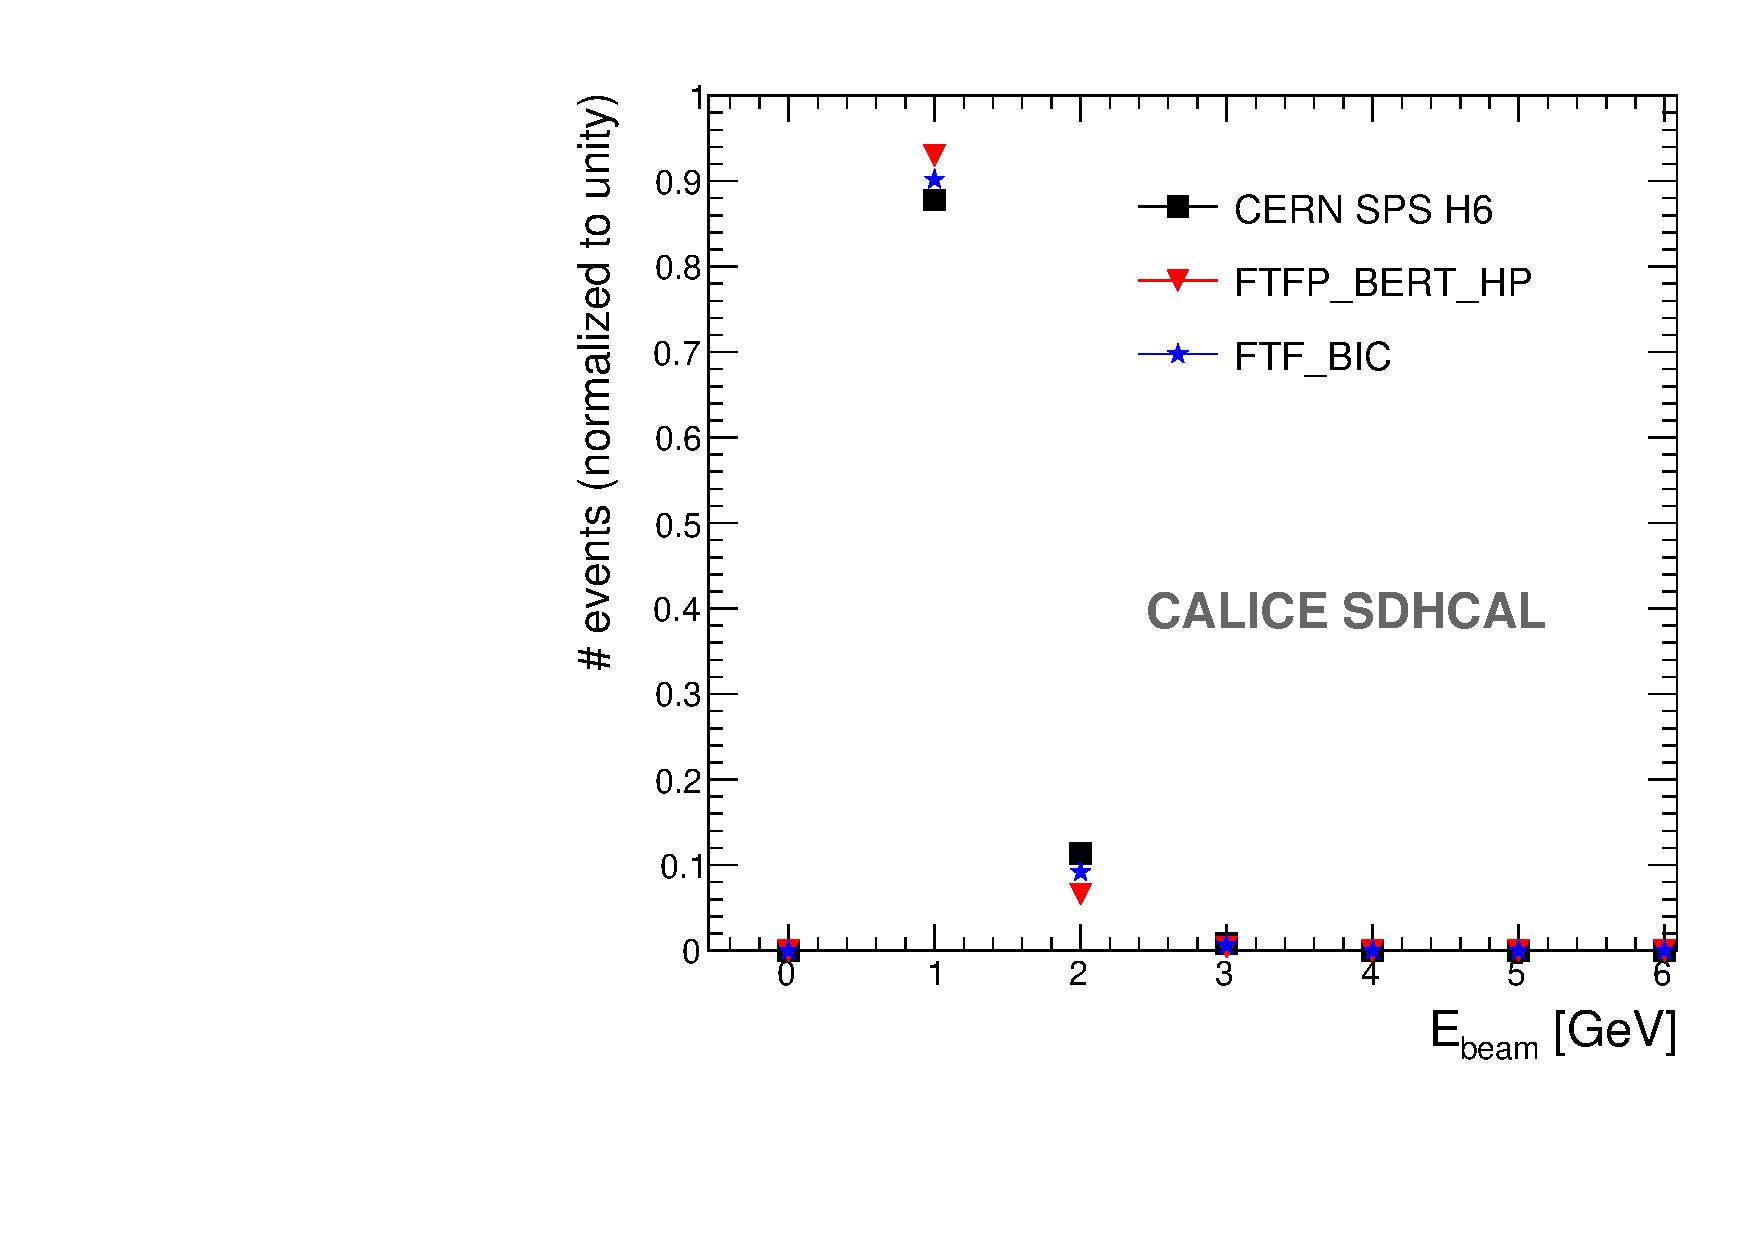
\includegraphics[width=0.48\textwidth]{plots/SingleParticle/CALICESDHCAL/MC_DATA_COMP/Single_MC_DATA_COMP_NPfos_20GeV.pdf}
    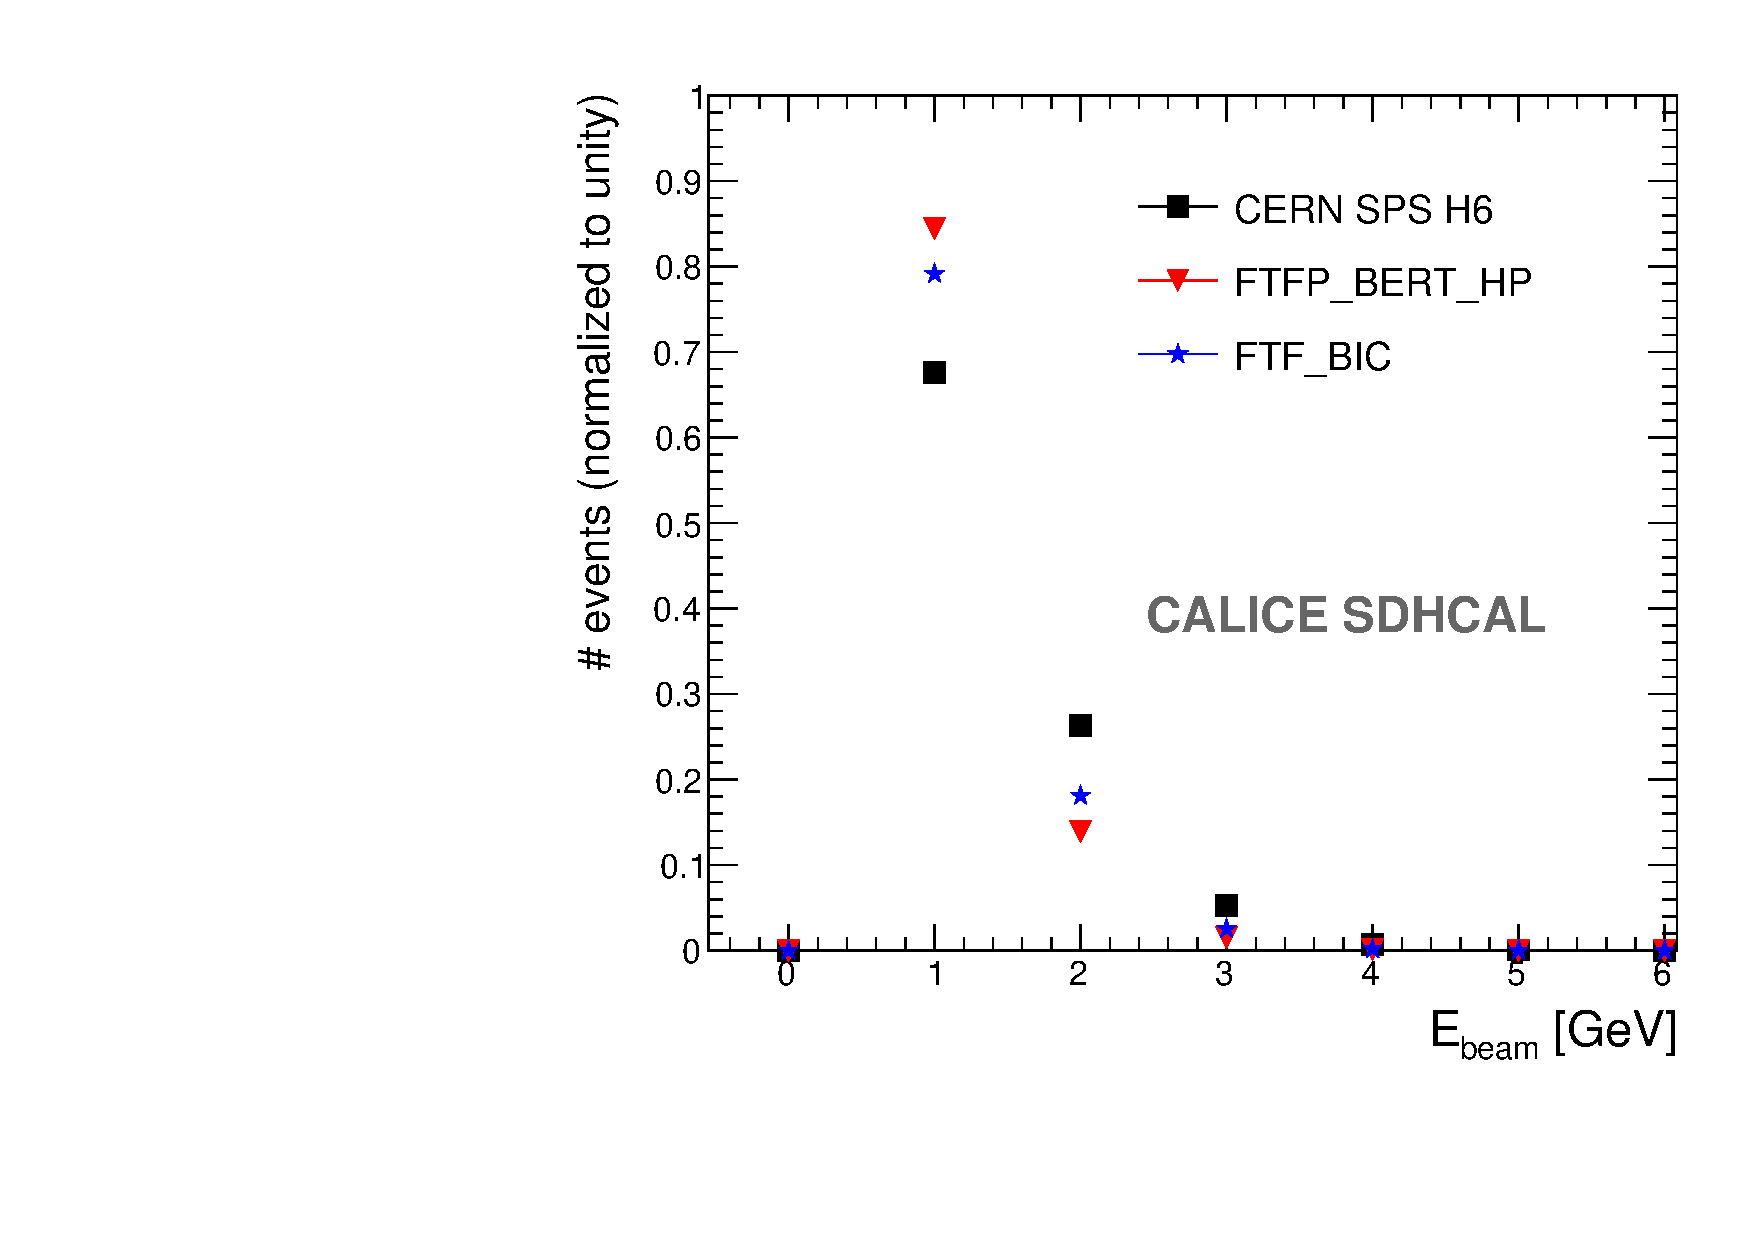
\includegraphics[width=0.48\textwidth]{plots/SingleParticle/CALICESDHCAL/MC_DATA_COMP/Single_MC_DATA_COMP_NPfos_70GeV.pdf} \\
  \end{center}
  \caption{\label{ARBOR_SINGLE_PARTICLE_NPFOS_20_AND_70_GEV} Distributions of the number of reconstructed particles for a 20 GeV single charged hadron (left) and a 70 GeV single charged hadron (right).}
\end{figure}

\begin{figure}[!h]
  \begin{center}
    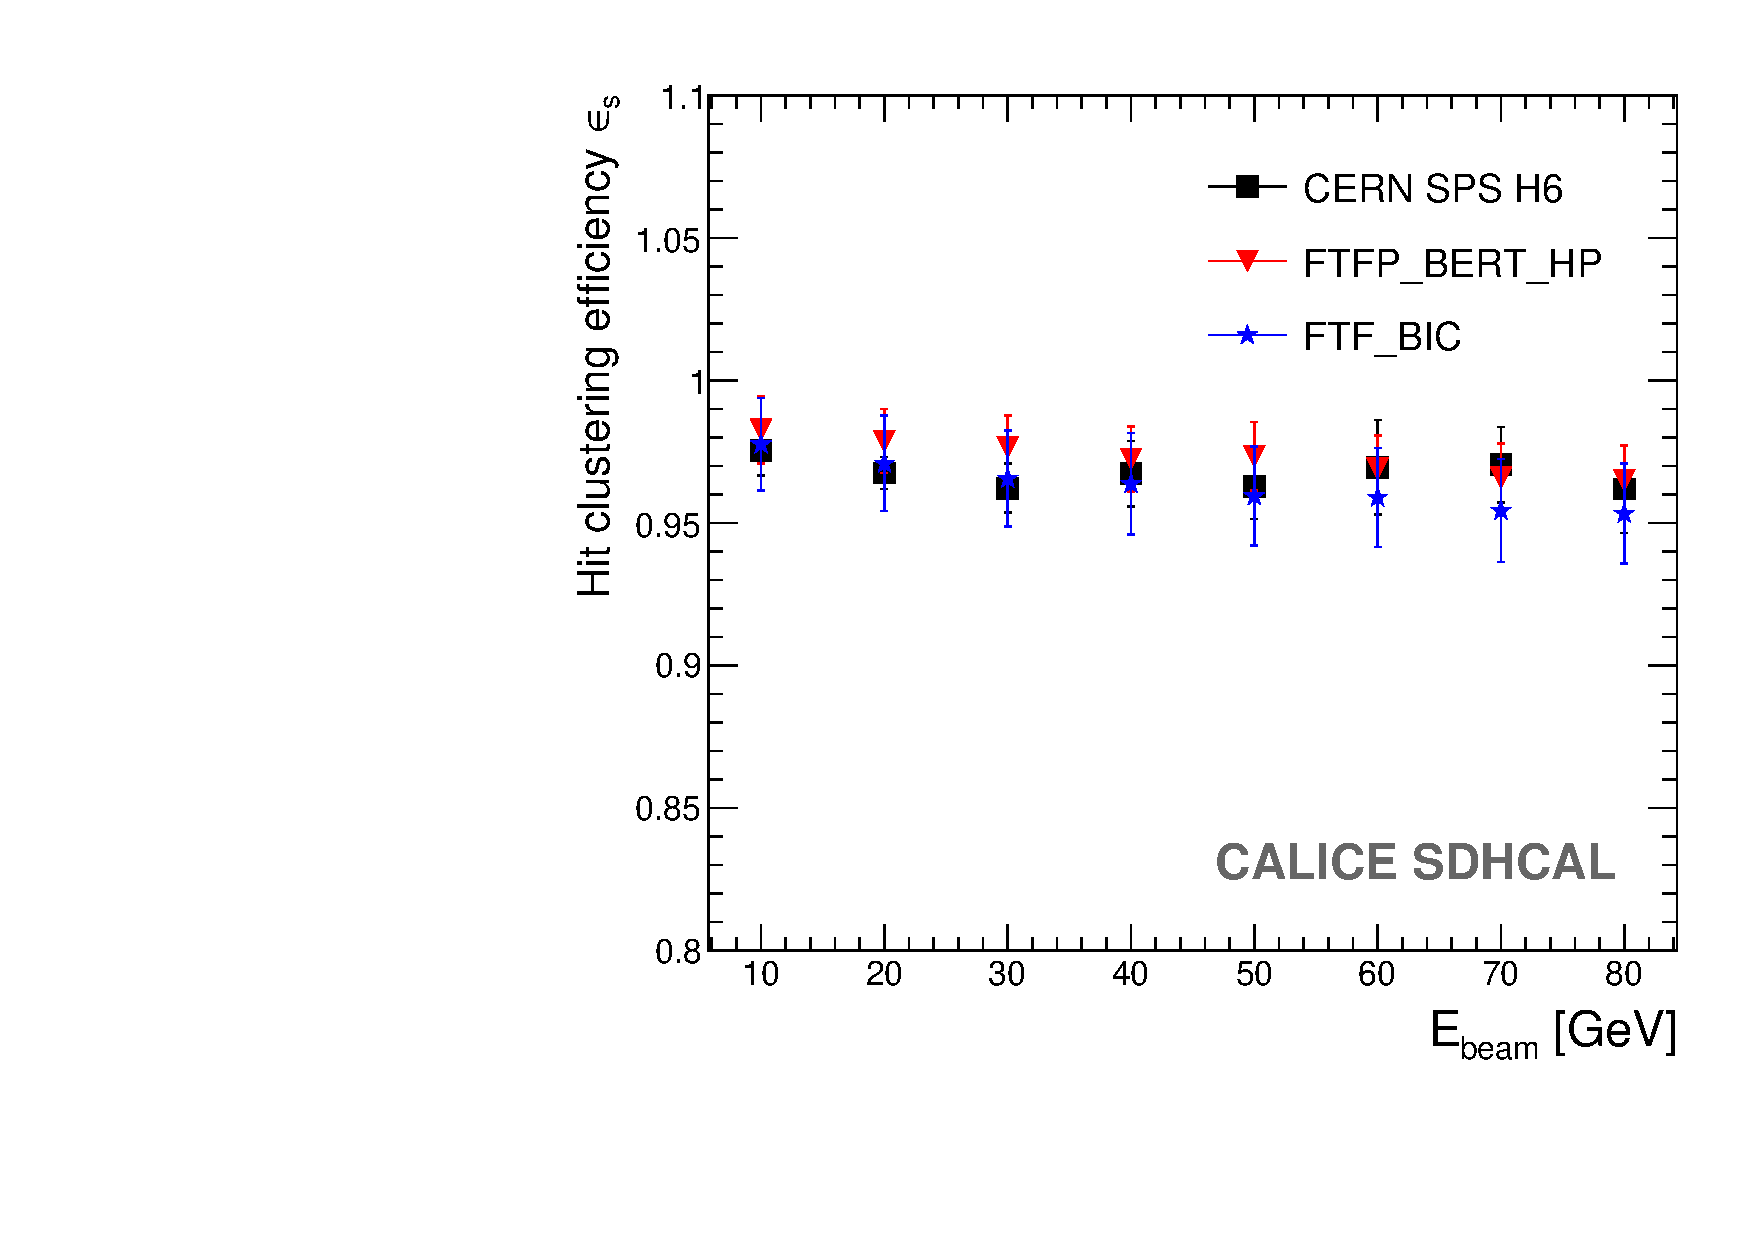
\includegraphics[width=0.48\textwidth]{plots/SingleParticle/CALICESDHCAL/MC_DATA_COMP/Single_MC_DATA_COMP_Efficiency.pdf}
    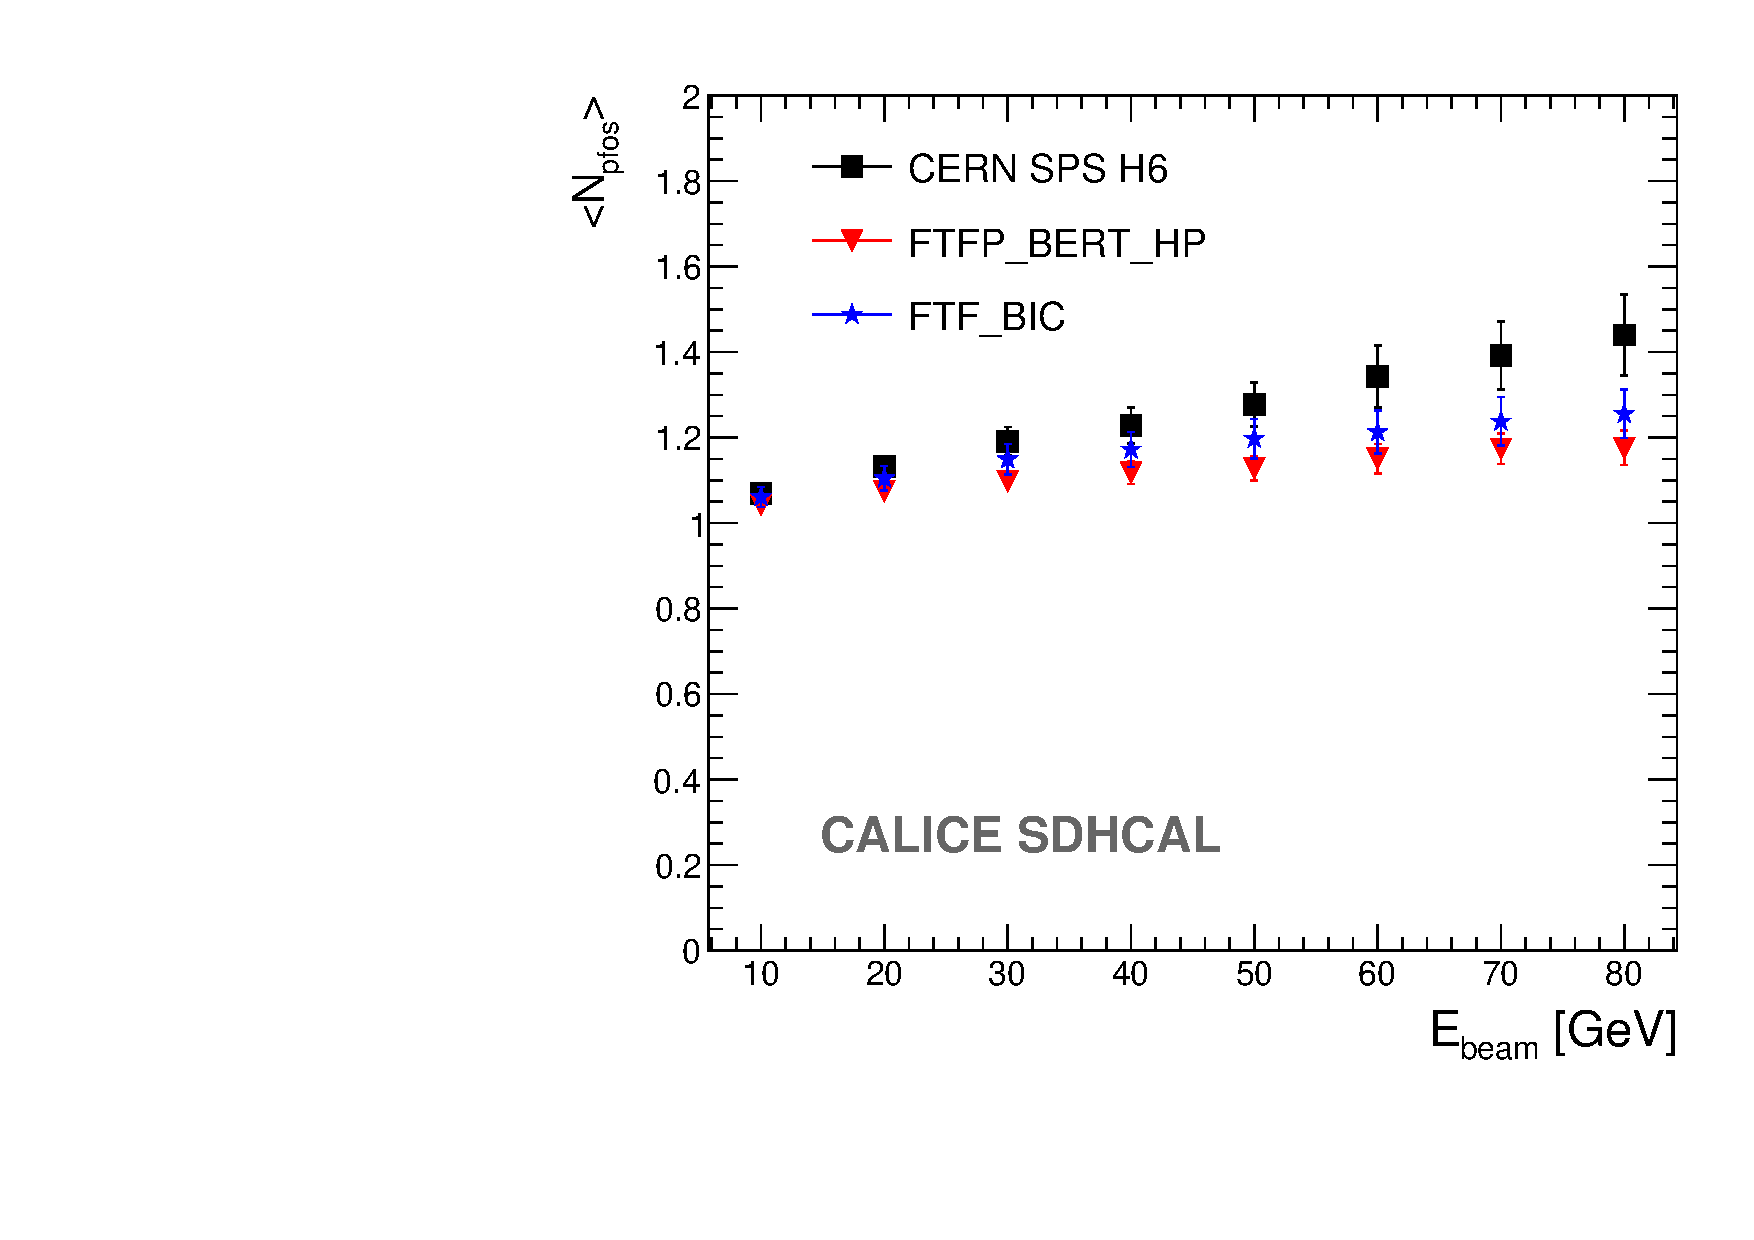
\includegraphics[width=0.48\textwidth]{plots/SingleParticle/CALICESDHCAL/MC_DATA_COMP/Single_MC_DATA_COMP_NPfos.pdf} \\
  \end{center}
  \caption{\label{ARBOR_SINGLE_PARTICLE_EFFICIENCY_AND_NPFOS} Hit clustering efficiency (left) and the mean number of reconstructed particles (right) after ArborPFA reconstruction on single pion shower events with the SDHCAL prototype using test beam data and simulation samples.}
\end{figure}

We define the efficiency of the single particle reconstruction, or the hit clustering efficiency $\epsilon_s$, as the fraction of hits recovered by the ArborPFA program and correctly attached to the track in front of the calorimeter. Figure \ref{ARBOR_SINGLE_PARTICLE_EFFICIENCY_AND_NPFOS} shows the mean efficiency of the single particle reconstruction (left) and the mean number of reconstructed particles (right) as a function of the beam energy after applying ArborPFA. Two typical distributions of the number of reconstructed particles are shown in figure \ref{ARBOR_SINGLE_PARTICLE_NPFOS_20_AND_70_GEV} as an example. The hit clustering efficiency shows a constant efficiency of over 95\% over the whole beam energy range for both test beam data and simulation samples. Since the number of hits increases with the energy, the number of missed hits in the reconstructed charged particle also increases. Consequently, the mean number of reconstructed particles shows an increase which is directly due to shower splitting. This number grows up to 1.45 for particles at 80 GeV for test beam data but has only a small impact on the reconstructed energy and energy resolution because the small additional clusters represent a small amount of energy.

%%%%%%%%%%%%%%%%%%
\begin{figure}[!h]
  \begin{center}
    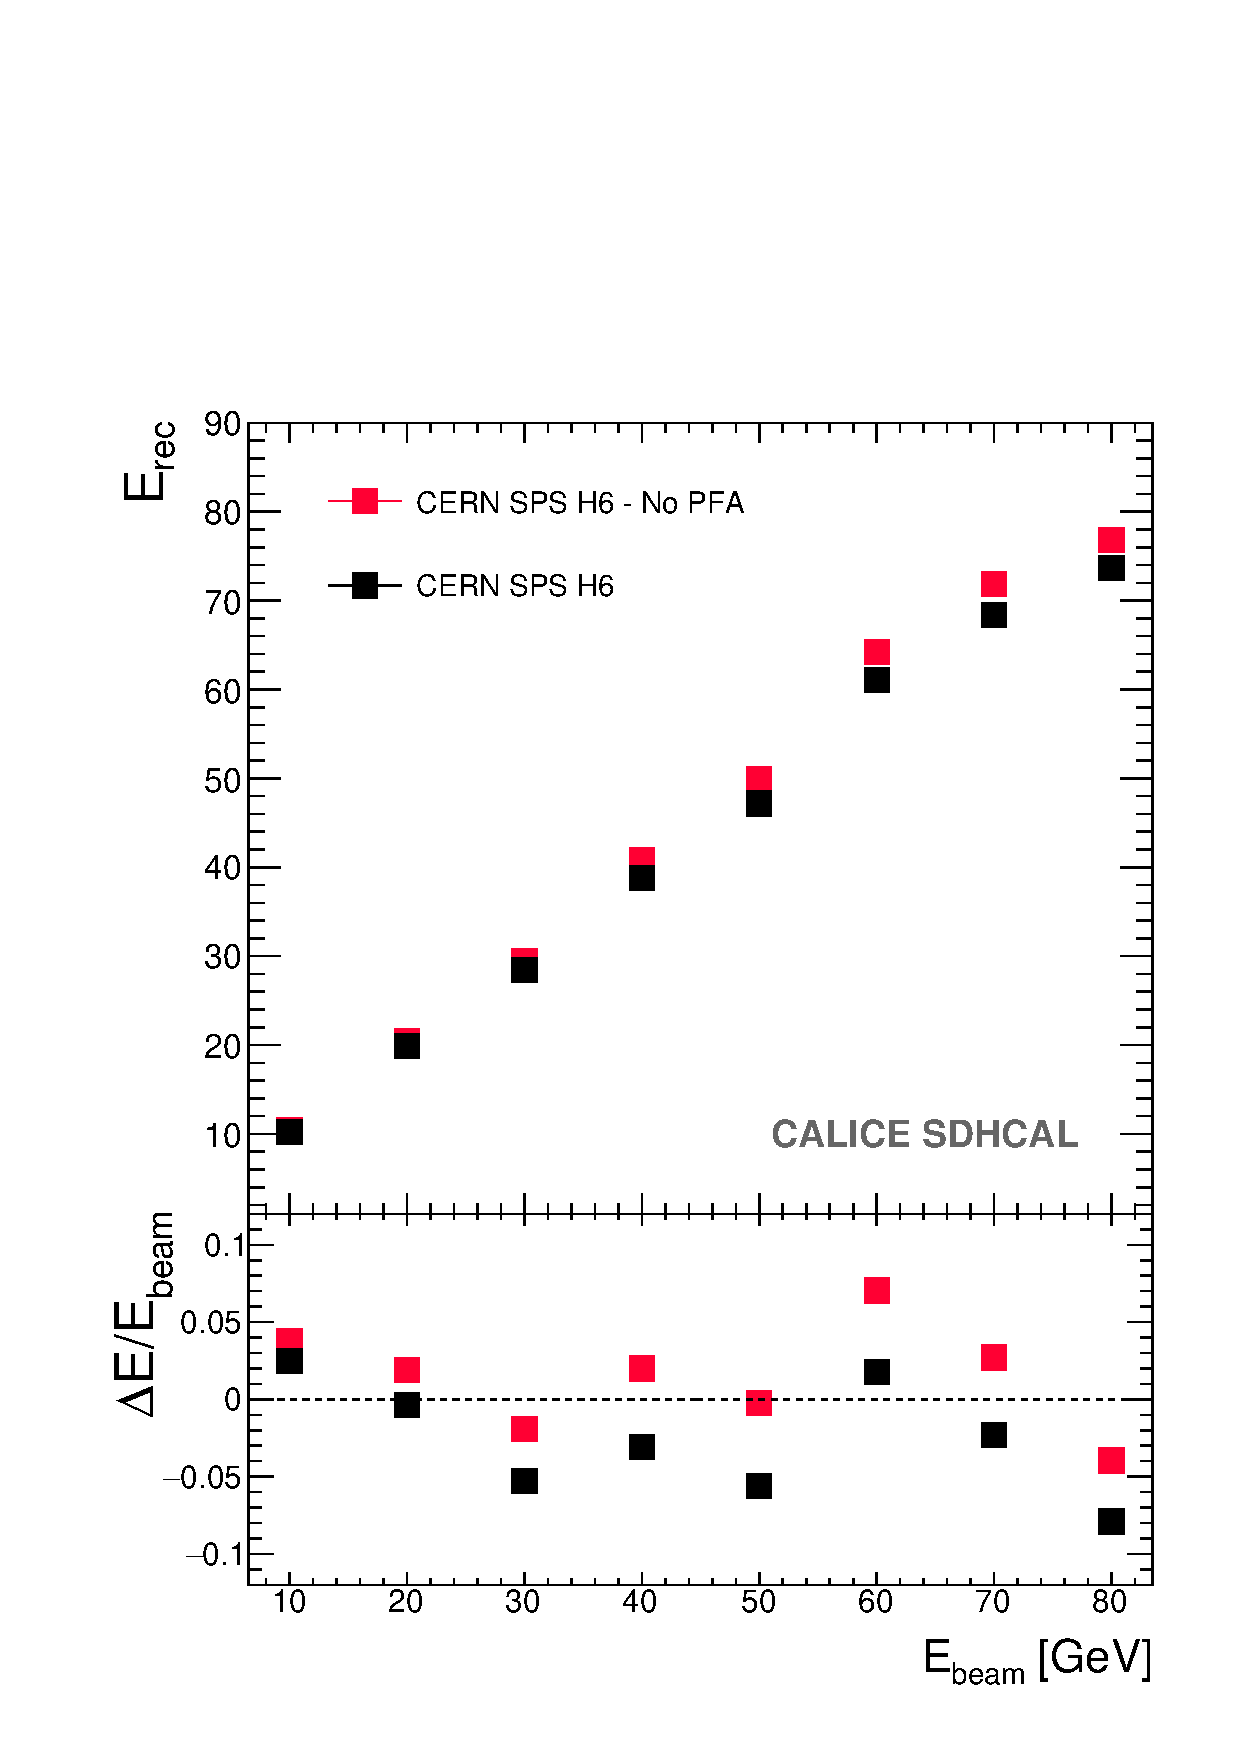
\includegraphics[width=0.48\textwidth]{plots/SingleParticle/CALICESDHCAL/DATA_ONLY/Single_DATA_ONLY_ERec.pdf}
    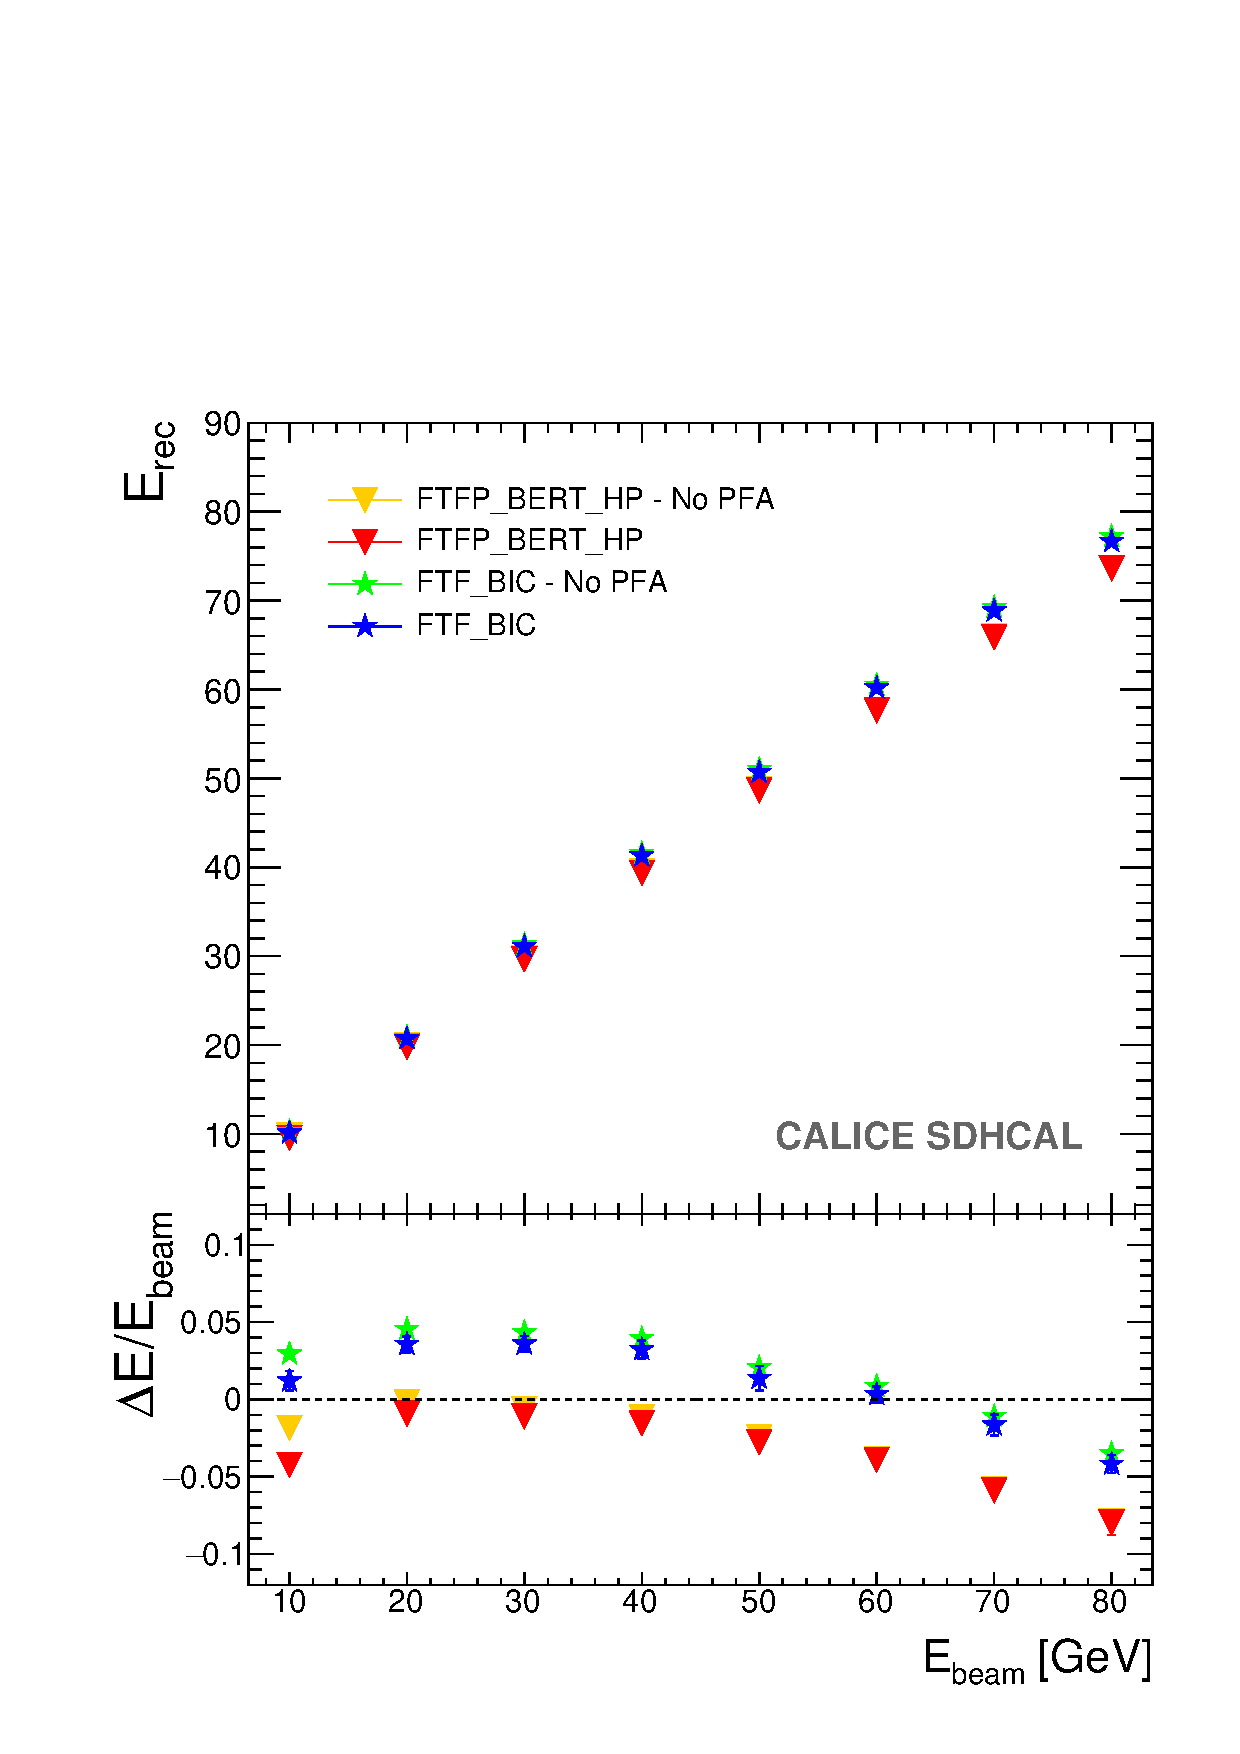
\includegraphics[width=0.48\textwidth]{plots/SingleParticle/CALICESDHCAL/MC_ONLY/Single_MC_ONLY_ERec.pdf} \\
  \end{center}
  \caption{\label{ARBOR_SINGLE_PARTICLE_EREC_DATA_MC} Reconstructed energy before and after ArborPFA reconstruction on single pion shower event for test beam data (left) and simulation data (right).}
\end{figure}

%%%%%%%%%%%%%%%%%%
\begin{figure}[!h]
  \begin{center}
    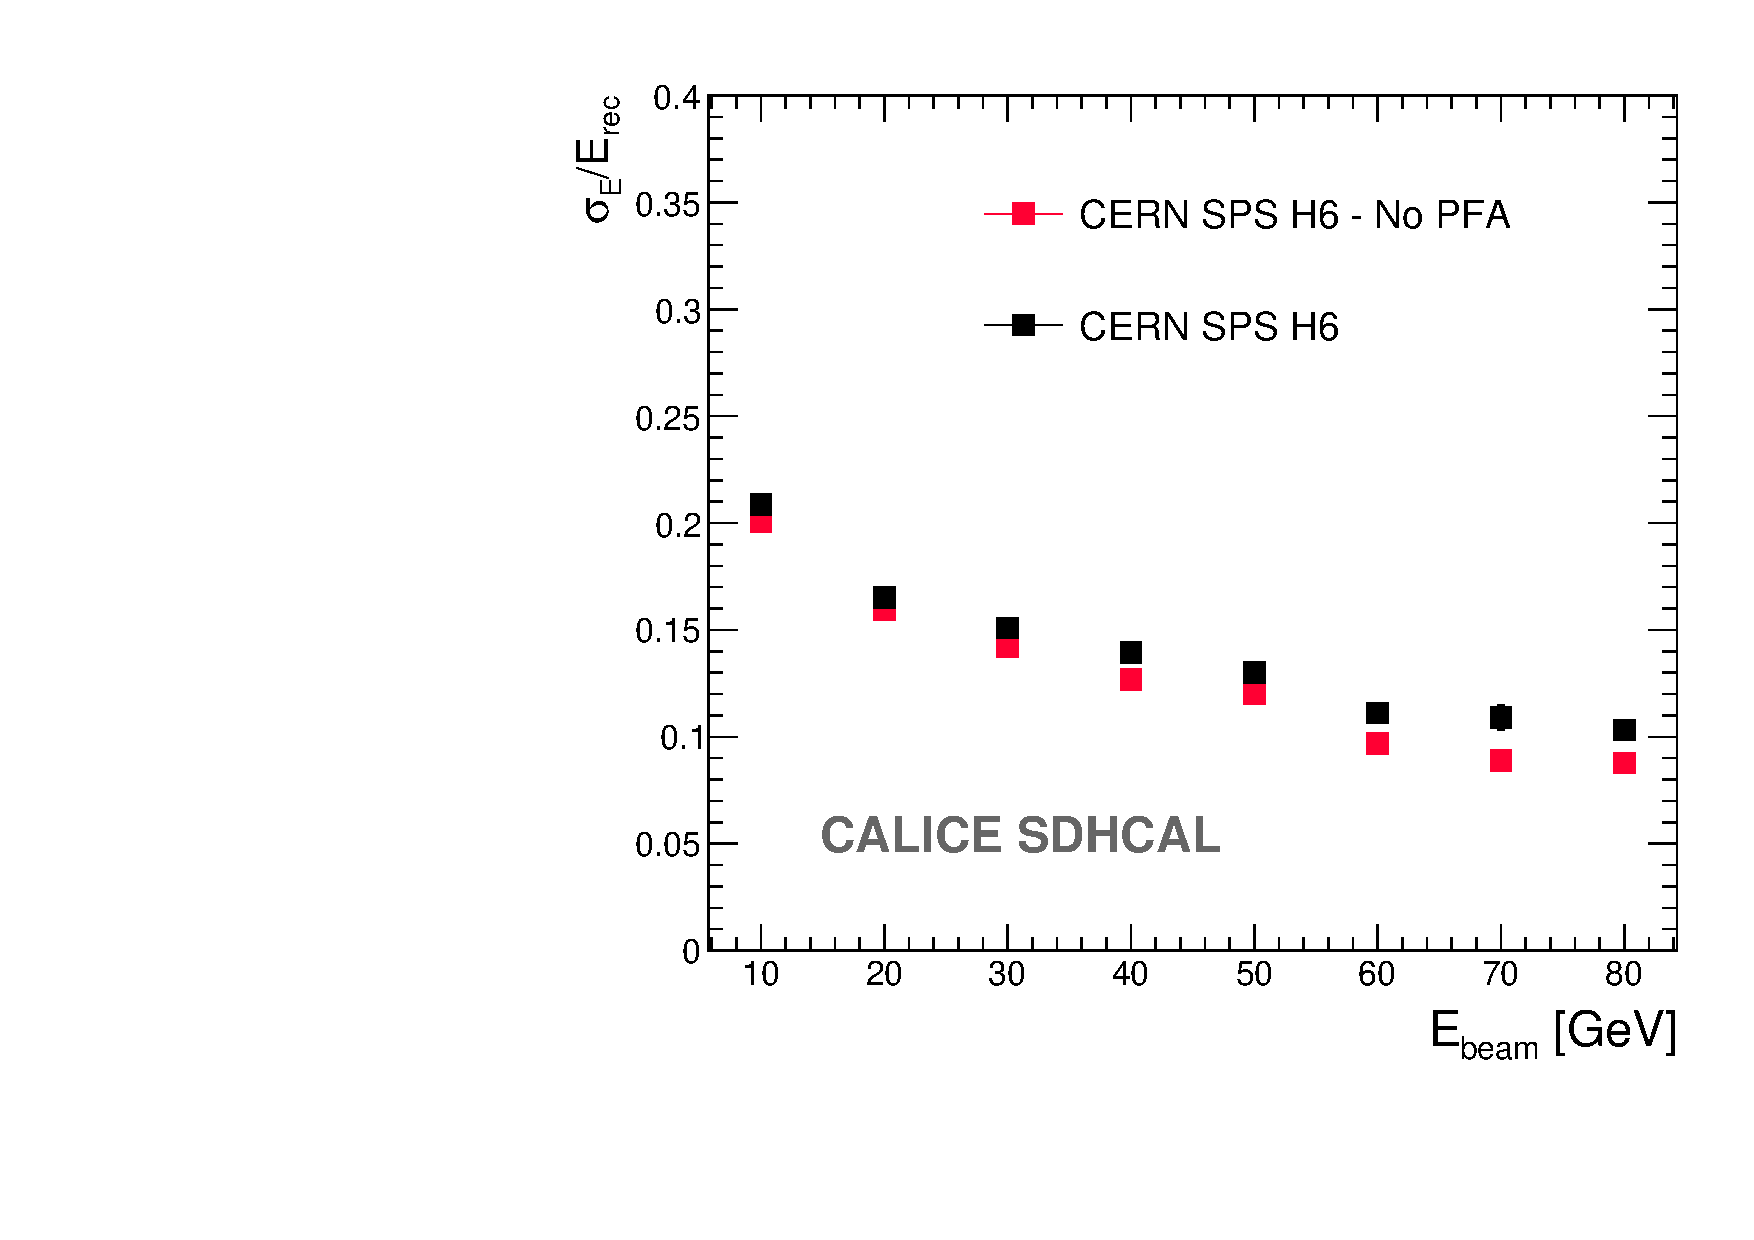
\includegraphics[width=0.48\textwidth]{plots/SingleParticle/CALICESDHCAL/DATA_ONLY/Single_DATA_ONLY_EResol.pdf}
    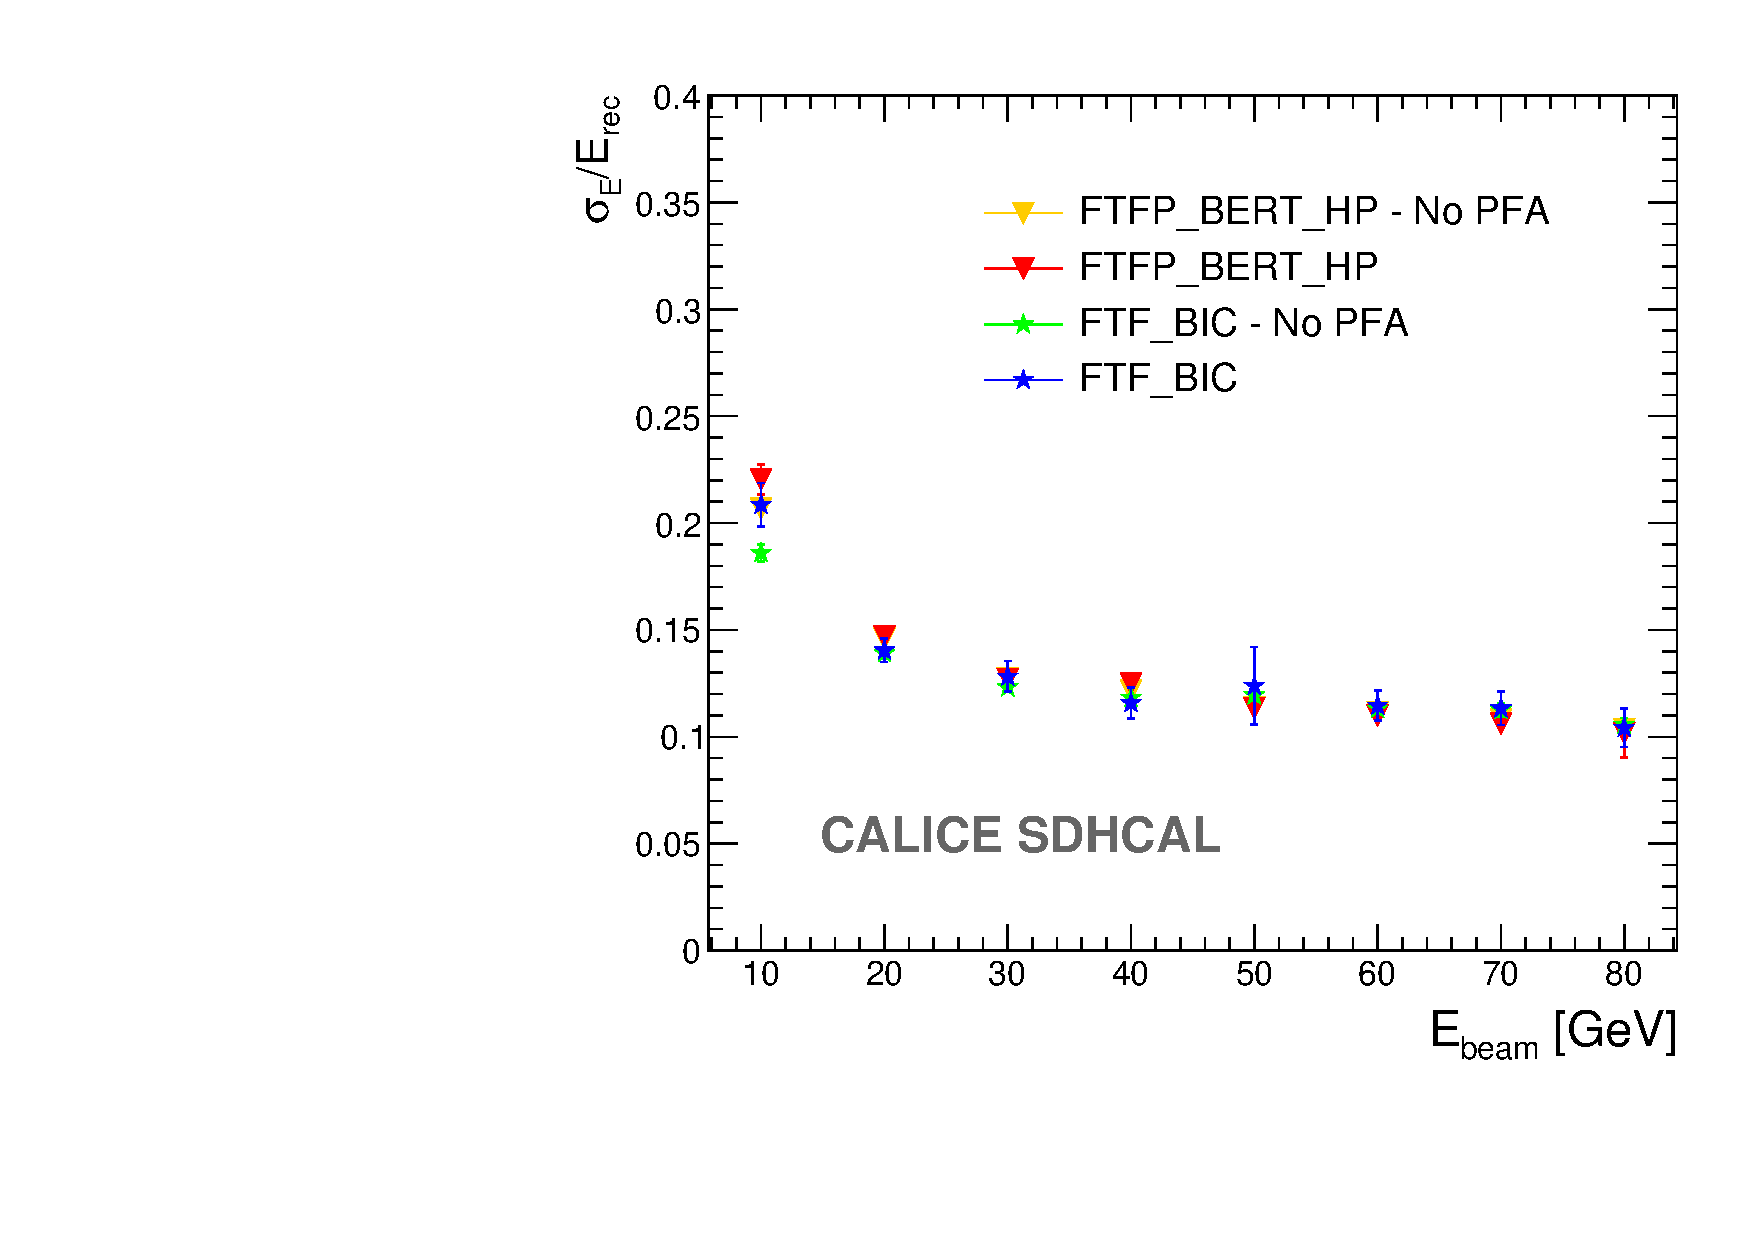
\includegraphics[width=0.48\textwidth]{plots/SingleParticle/CALICESDHCAL/MC_ONLY/Single_MC_ONLY_EResol.pdf} \\
  \end{center}
  \caption{\label{ARBOR_SINGLE_PARTICLE_ERESOL_DATA_MC} Energy resolution before and after ArborPFA reconstruction on single pion shower event for simulation data (left) and test beam data (right).}
\end{figure}

%%%%%%%%%%%%%%%%%%
\begin{figure}[!h]
  \begin{center}
    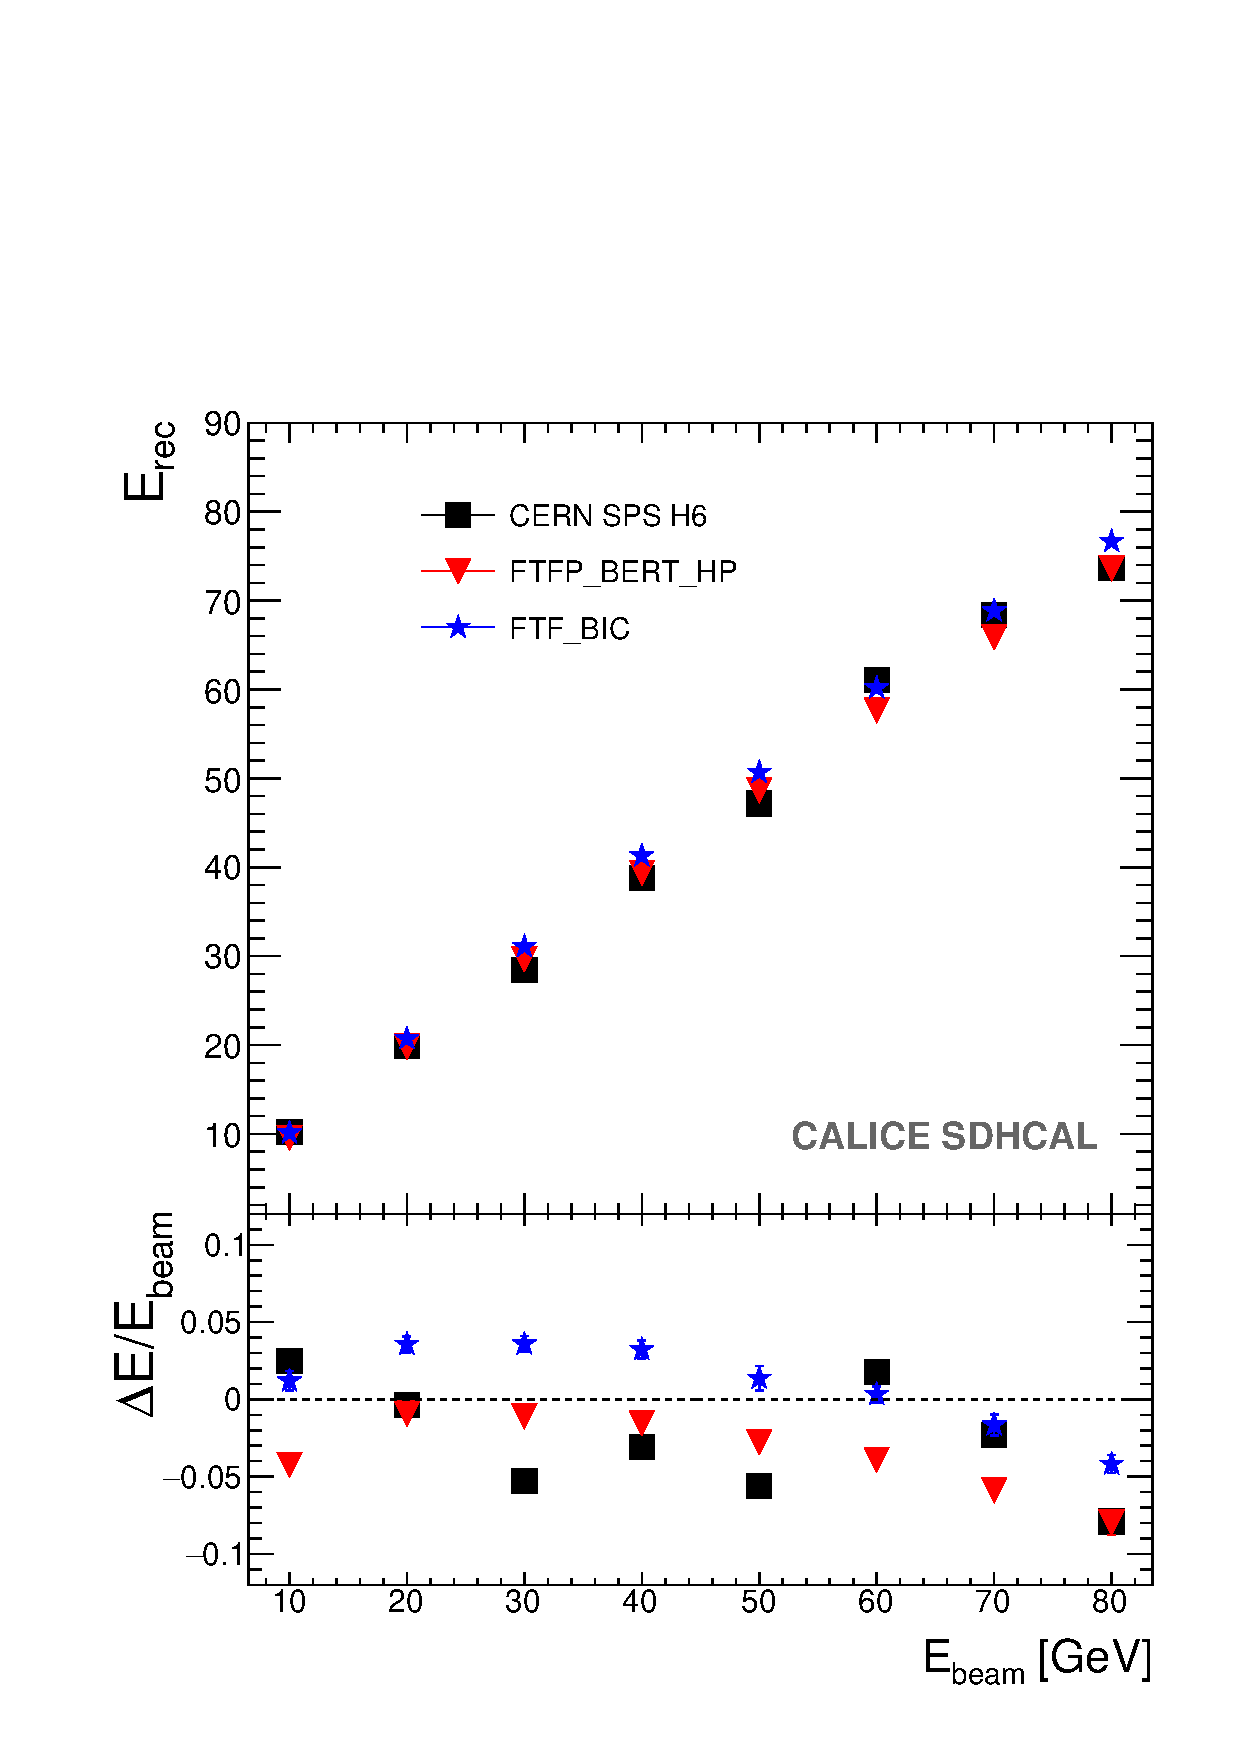
\includegraphics[width=0.48\textwidth]{plots/SingleParticle/CALICESDHCAL/MC_DATA_COMP/Single_MC_DATA_COMP_ERec.pdf}
    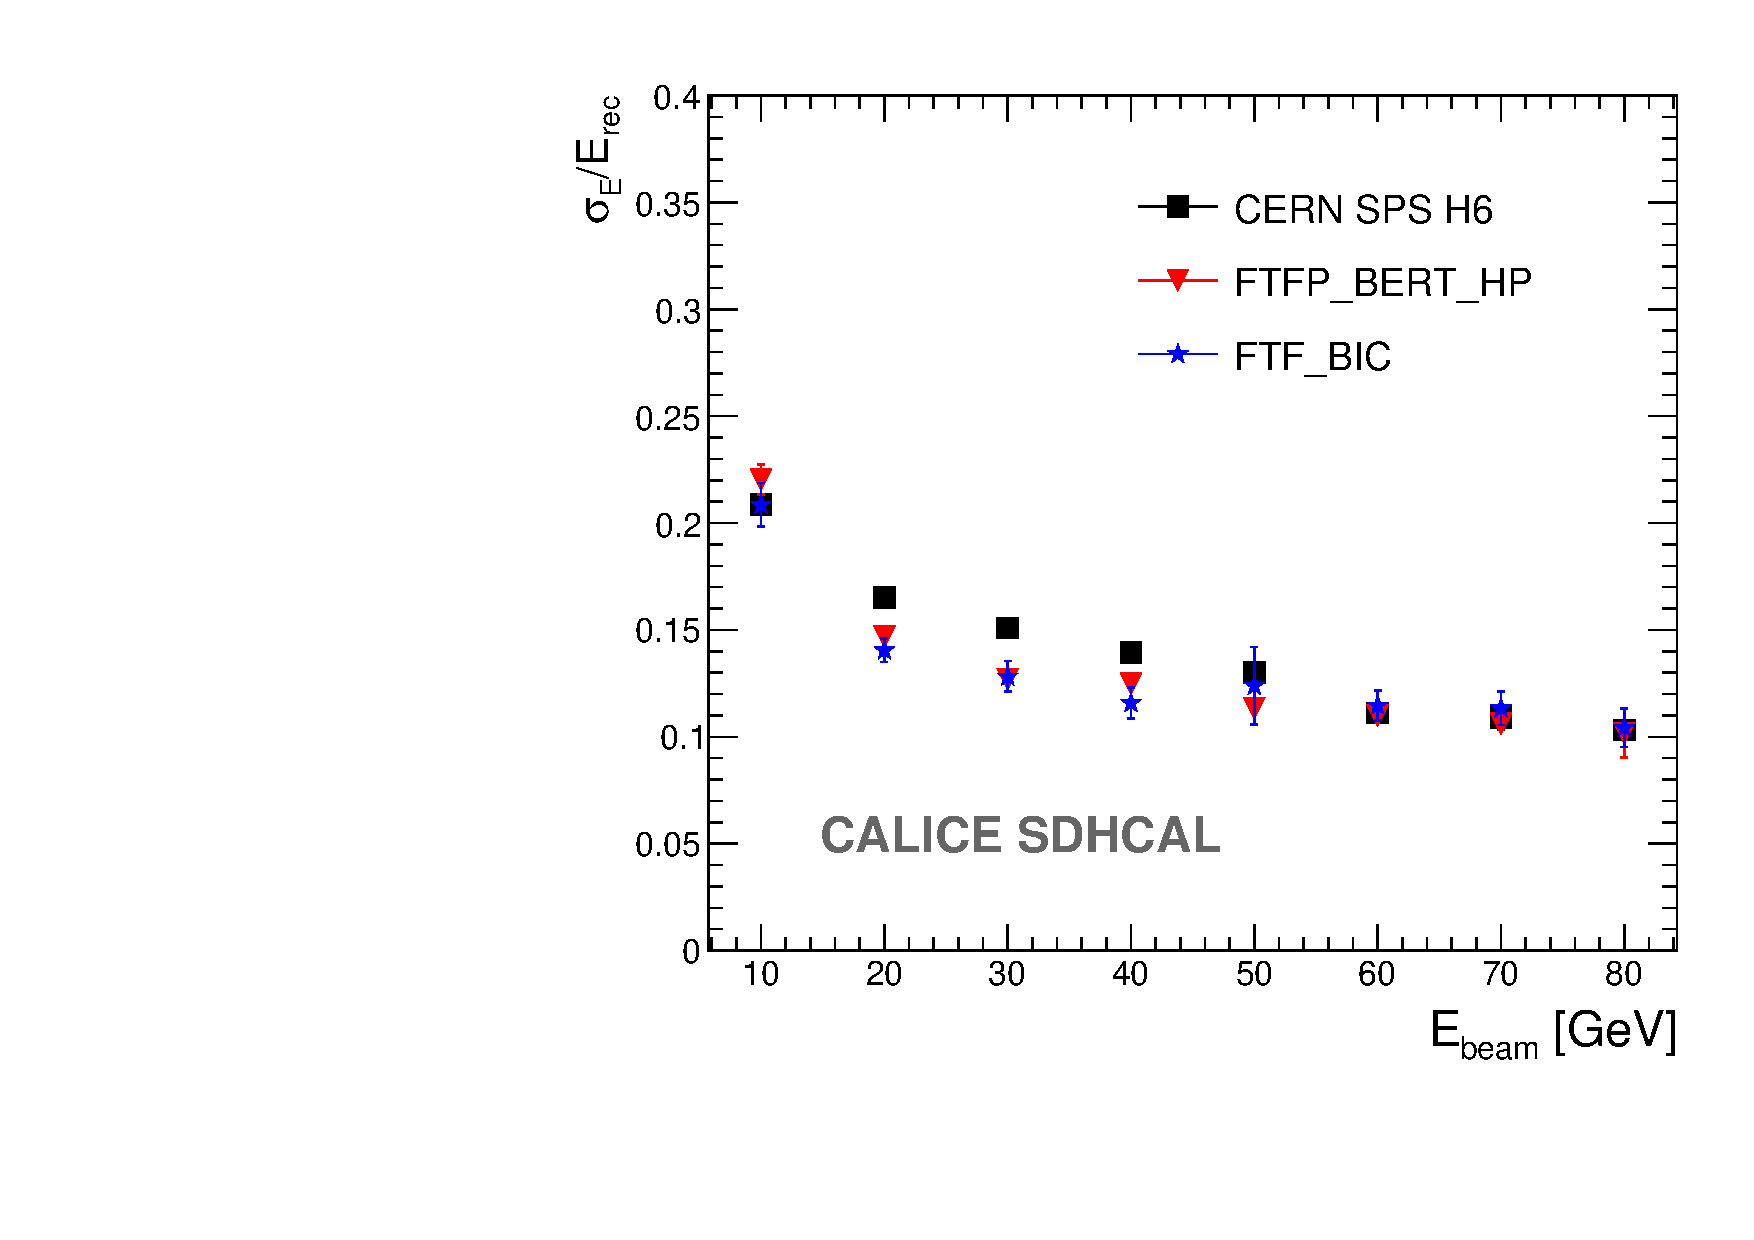
\includegraphics[width=0.48\textwidth]{plots/SingleParticle/CALICESDHCAL/MC_DATA_COMP/Single_MC_DATA_COMP_EResol.pdf} \\
  \end{center}
  \caption{\label{ARBOR_SINGLE_PARTICLE_EREC_AND_ERESOL_COMP} Reconstructed energy (left) and energy resolution (right) after ArborPFA reconstruction on single pion shower event with the SDHCAL prototype.}
\end{figure}

Figures \ref{ARBOR_SINGLE_PARTICLE_EREC_DATA_MC} and \ref{ARBOR_SINGLE_PARTICLE_ERESOL_DATA_MC} show respectively the reconstructed energy and energy resolution of a single charged pion before and after running the ArborPFA program on test beam data (left) and simulation data (right). For an easier comparison between test beam and simulation reconstruction, figure \ref{ARBOR_SINGLE_PARTICLE_EREC_AND_ERESOL_COMP} shows the same two variables on the same plot.

These energy points are extracted using two fits of the energy distributions : i) a gaussian distribution fit over the full reconstructed distribution is first performed. The mean $\mu_{E,first}$ and width $\sigma_{E,first}$ are extracted, and ii) a second gaussian fit is then performed over the range [$\mu_{E,first}$-1.5*$\sigma_{E,first}$ ; $\mu_{E,first}$+1.5*$\sigma_{E,first}$]. From the latter, we extract the final values of the reconstructed energy and energy resolution defined as the mean $\mu_E$ and the width $\sigma_E$ respectively of the gaussian fit (same procedure as applied in \cite{sdhcal-paper}). 
The deviation from linearity is shown below the reconstructed energy and is defined as :

\begin{equation}
  \Delta E/E_{beam} = \Big(\mu_{E} - E_{beam}\Big)/E_{beam}
\end{equation}

The efficiency plot has shown that some hits are missing after reconstruction so it is expected to have a small energy decrease in the reconstructed energy. Nevertheless, the linearity is still within 8\% as before applying the reconstruction. The energy resolution is also not so much affected after reconstruction.

%%%%%%%%%%%%%%%%%%%%%%%%%%%%%%%%%%%%%%%%%%%%%%%%%%%%%
%%%% Separation of two close-by hadronic showers %%%%
%%%%%%%%%%%%%%%%%%%%%%%%%%%%%%%%%%%%%%%%%%%%%%%%%%%%%
%\newpage
\section{Separation of two close-by hadronic showers}
\label{OVERLAY_EVENT_SECTION}

The ability of a particle flow algorithm to disentangle nearby showers is a key point for the reconstruction in detectors such as ILD of the ILC. To study the confusion between neutral and charged hadrons and the ability of the ArborPFA algorithm to disentangle them, we again use the same test beam data and simulation samples of the SDHCAL prototype. Two different pion showers are first overlaid in the same event and the ArborPFA algorithm is run on the overlaid event with the same parameters as for the single particle study. An analysis of the separation is then performed in order to evaluate the ability of the algorithm to disentangle two nearby hadronic showers.

%%%%%%%%%%%%%%%%%%%%%%%%%%%%%%%%%%%%%%%%%%%
%%%%%%%%%%%%%%%%%%%%%%%%%%%%%%%%%%%%%%%%%%%
\subsection{Overlay procedure and setup}

In order to study the separation of nearby hadronic showers, two events from test beam data or from simulation are overlaid in one event. We have chosen to overlay 10 GeV pion events and pion events with energies of 10 GeV and 30 GeV. The choice of these energies is motivated by the fact that it is the typical single particle energy range foreseen at the ILC within jets \cite{hadron-jets}. The distance between shower entry points is chosen to be between 5 cm and 30 cm with steps of 5 cm. A distance of 30 cm between showers means well identified energy depositions in the point of view of the reconstruction algorithm whereas 10 cm and 5 cm implies a contact between the showers and confusions for the reconstruction algorithm. 

The overlay event algorithm is processed as follow :

\begin{enumerate}
  \item The entering track segment of each shower is determined as for the single particle case. This allows to identify the entering points and starting points of each shower.
  \item The hits belonging to the 10 GeV pion primary track segment are removed from the event in order to emulate a neutral hadron shower.
  \item The two showers are then centred along the X and Y axis at the center of the calorimeter. No shift is performed on the Z direction (beam line).
  \item The showers are then shifted along the X axis by a distance of -d/2 for the neutral hadron and +d/2 for the charged particle, where d is the distance to the calorimeter center in cm.
  \item The two events are then overlaid. At this step a problem may occur : while mixing the showers in the event, pair of hits may overlap in the same cell. Knowing that we are using a semi digital readout and that the information of the deposit charge in each cell is not available in the data, we need to assign a new threshold by using an approximation. The most intuitive one is to keep the highest threshold of the two hits. Figure \ref{OVERLAY_EVENT_MC_EREC_OVERLAID_HITS} shows the reconstructed energy of the 10 GeV fake neutral hadron overlaid with a 30 GeV charged hadron at 30 cm distance (black) and 5 cm distance (red). The latter case is the worst one that can appear in this study given the energy points and the distances we have chosen. The maximum mean energy difference observed is about 0.2 GeV for the FTFP\_BERT\_HP simulation, which corresponds, given the table \ref{SDHCAL_ENERGY_MINIMIZATION_PARAMS}, to almost two hits of threshold 3 wrongly assigned. The effect of this approximation is thus negligible.
  \item The hits are tagged with respect to our initial showers. The overlaid hits are tagged differently so that the information on the overlaid hits can be retrieved after reconstruction.
  \item A new event is created containing the overlaid showers and the entering point of the charged particle track after shifting. An example is shown on figure \ref{OVERLAY_EVENT_DISPLAY}.
\end{enumerate}

\begin{figure}[!h]
  \begin{center}
    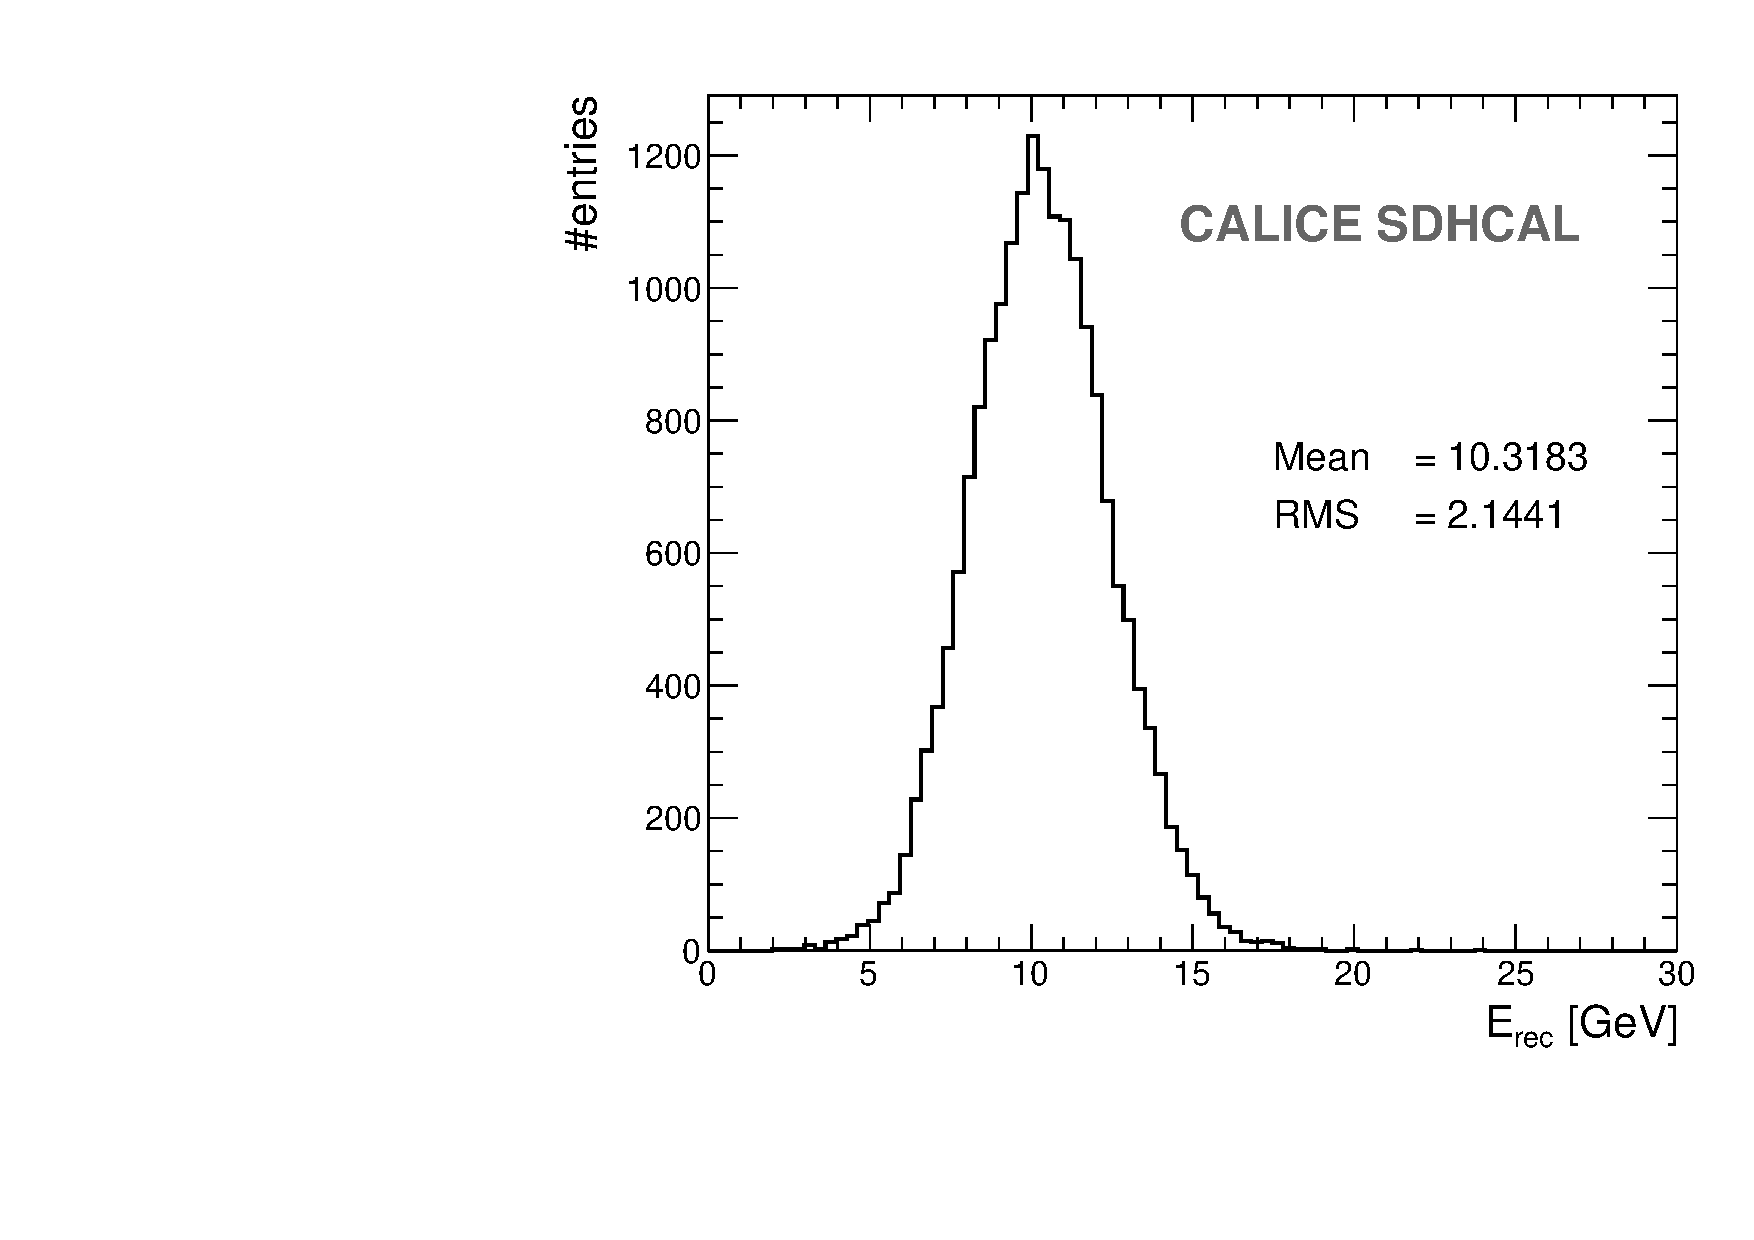
\includegraphics[width=0.45\linewidth]{plots/OverlayEvent/OverlayEvent_OverlayCheck_ChBefore_TB.pdf}
    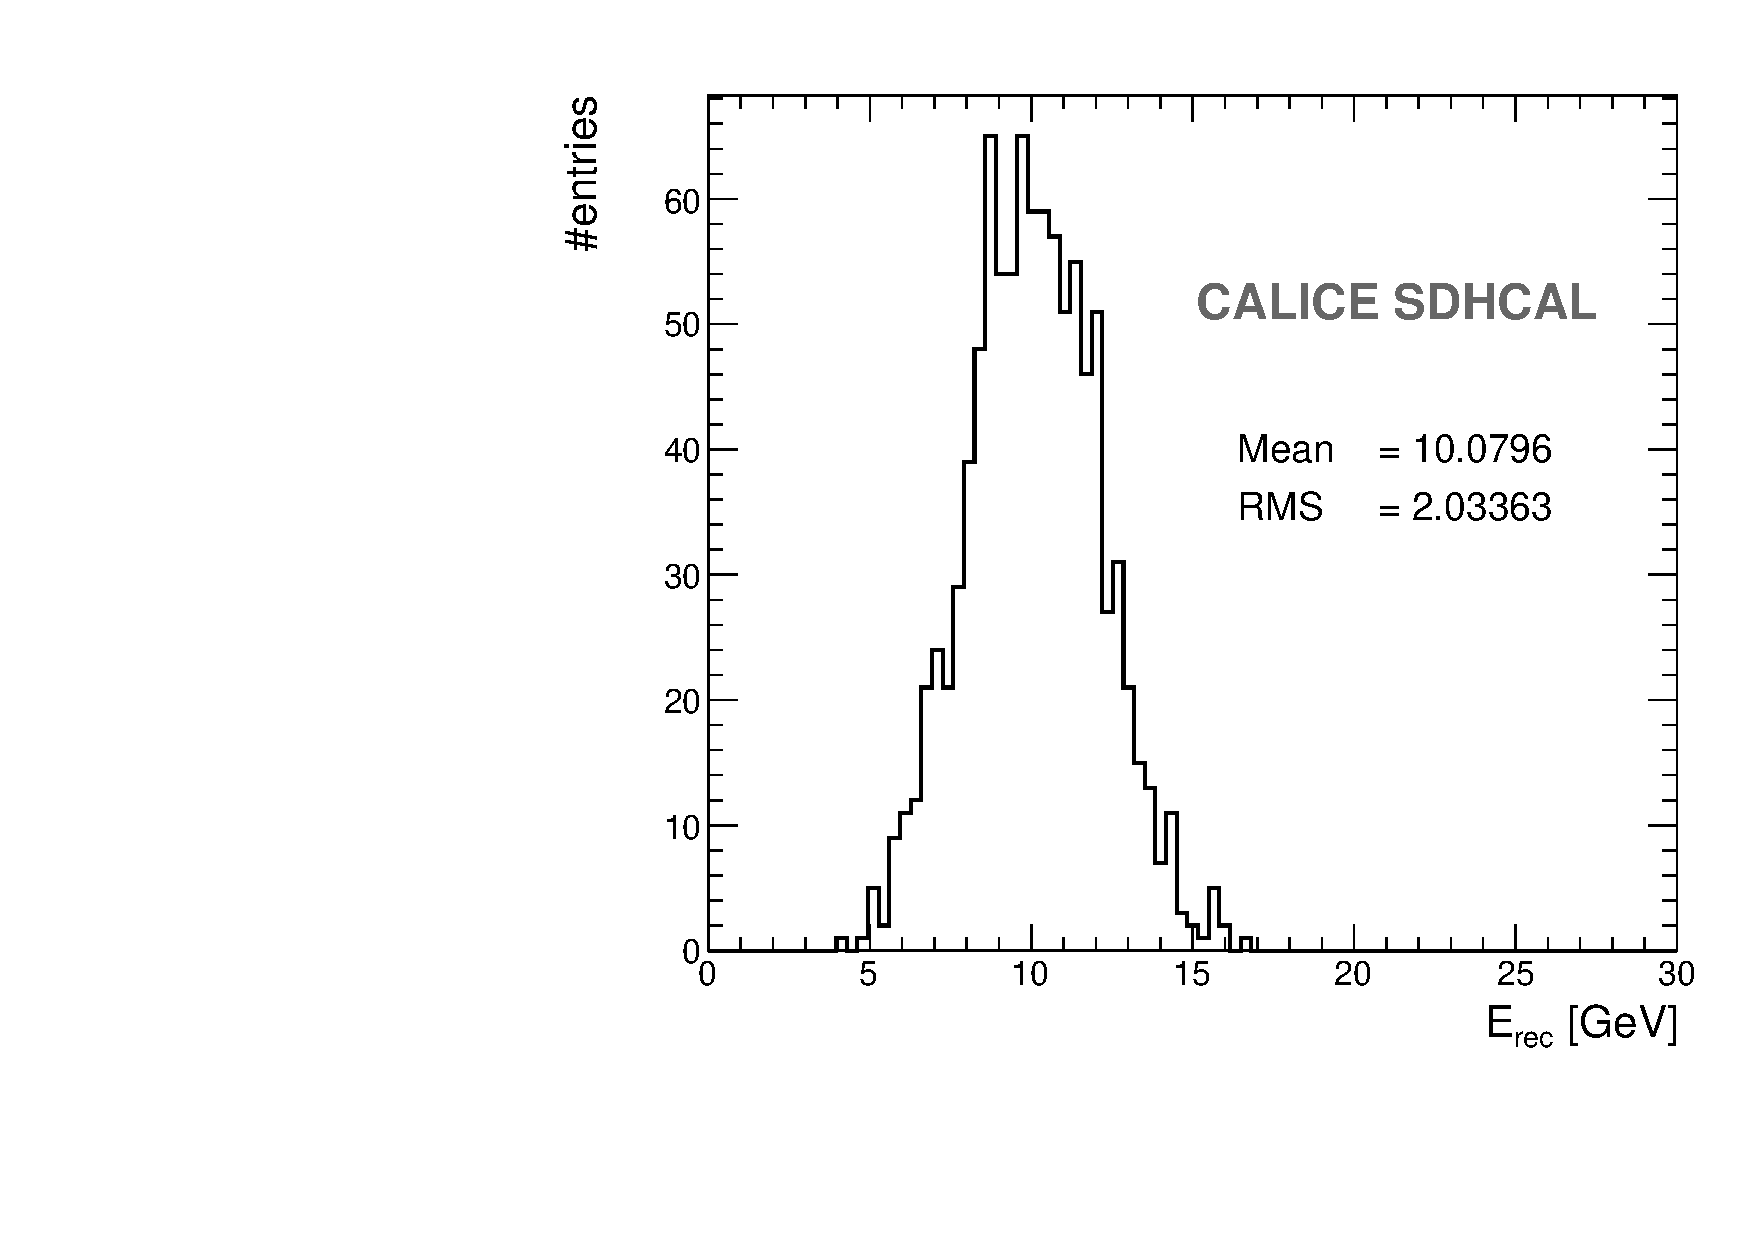
\includegraphics[width=0.45\linewidth]{plots/OverlayEvent/OverlayEvent_OverlayCheck_ChBefore_FTF_BIC.pdf}
    %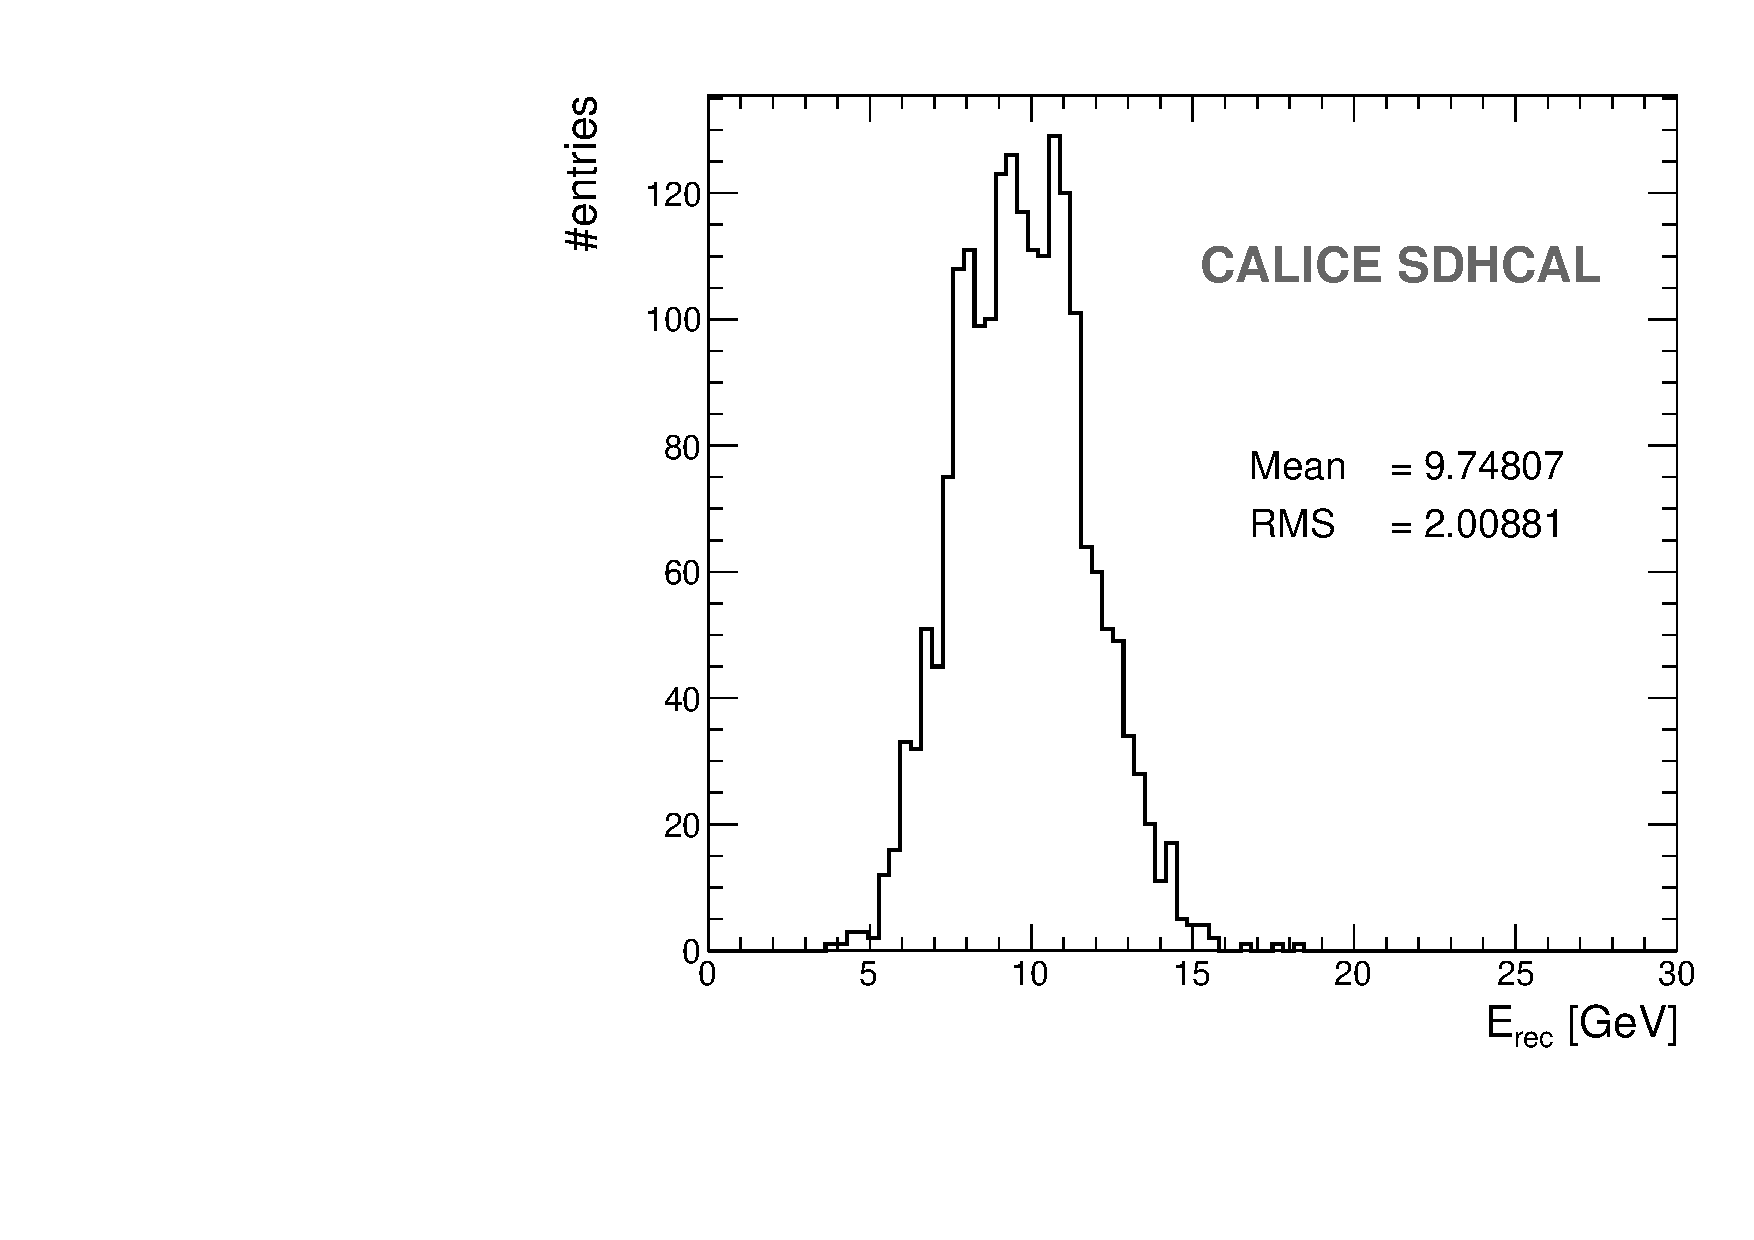
\includegraphics[width=0.32\linewidth]{plots/OverlayEvent/OverlayEvent_OverlayCheck_ChBefore_FTFP_BERT_HP.pdf}
  \end{center}
  \caption{\label{OVERLAY_EVENT_MC_CH_EREC_NO_OVERLAY} The reconstructed energy of a 10 GeV charged hadron before the overlay procedure for different data samples : test beam data (left) and FTF\_BIC simulation (right)}
\end{figure}

\begin{figure}[!h]
  \begin{center}
    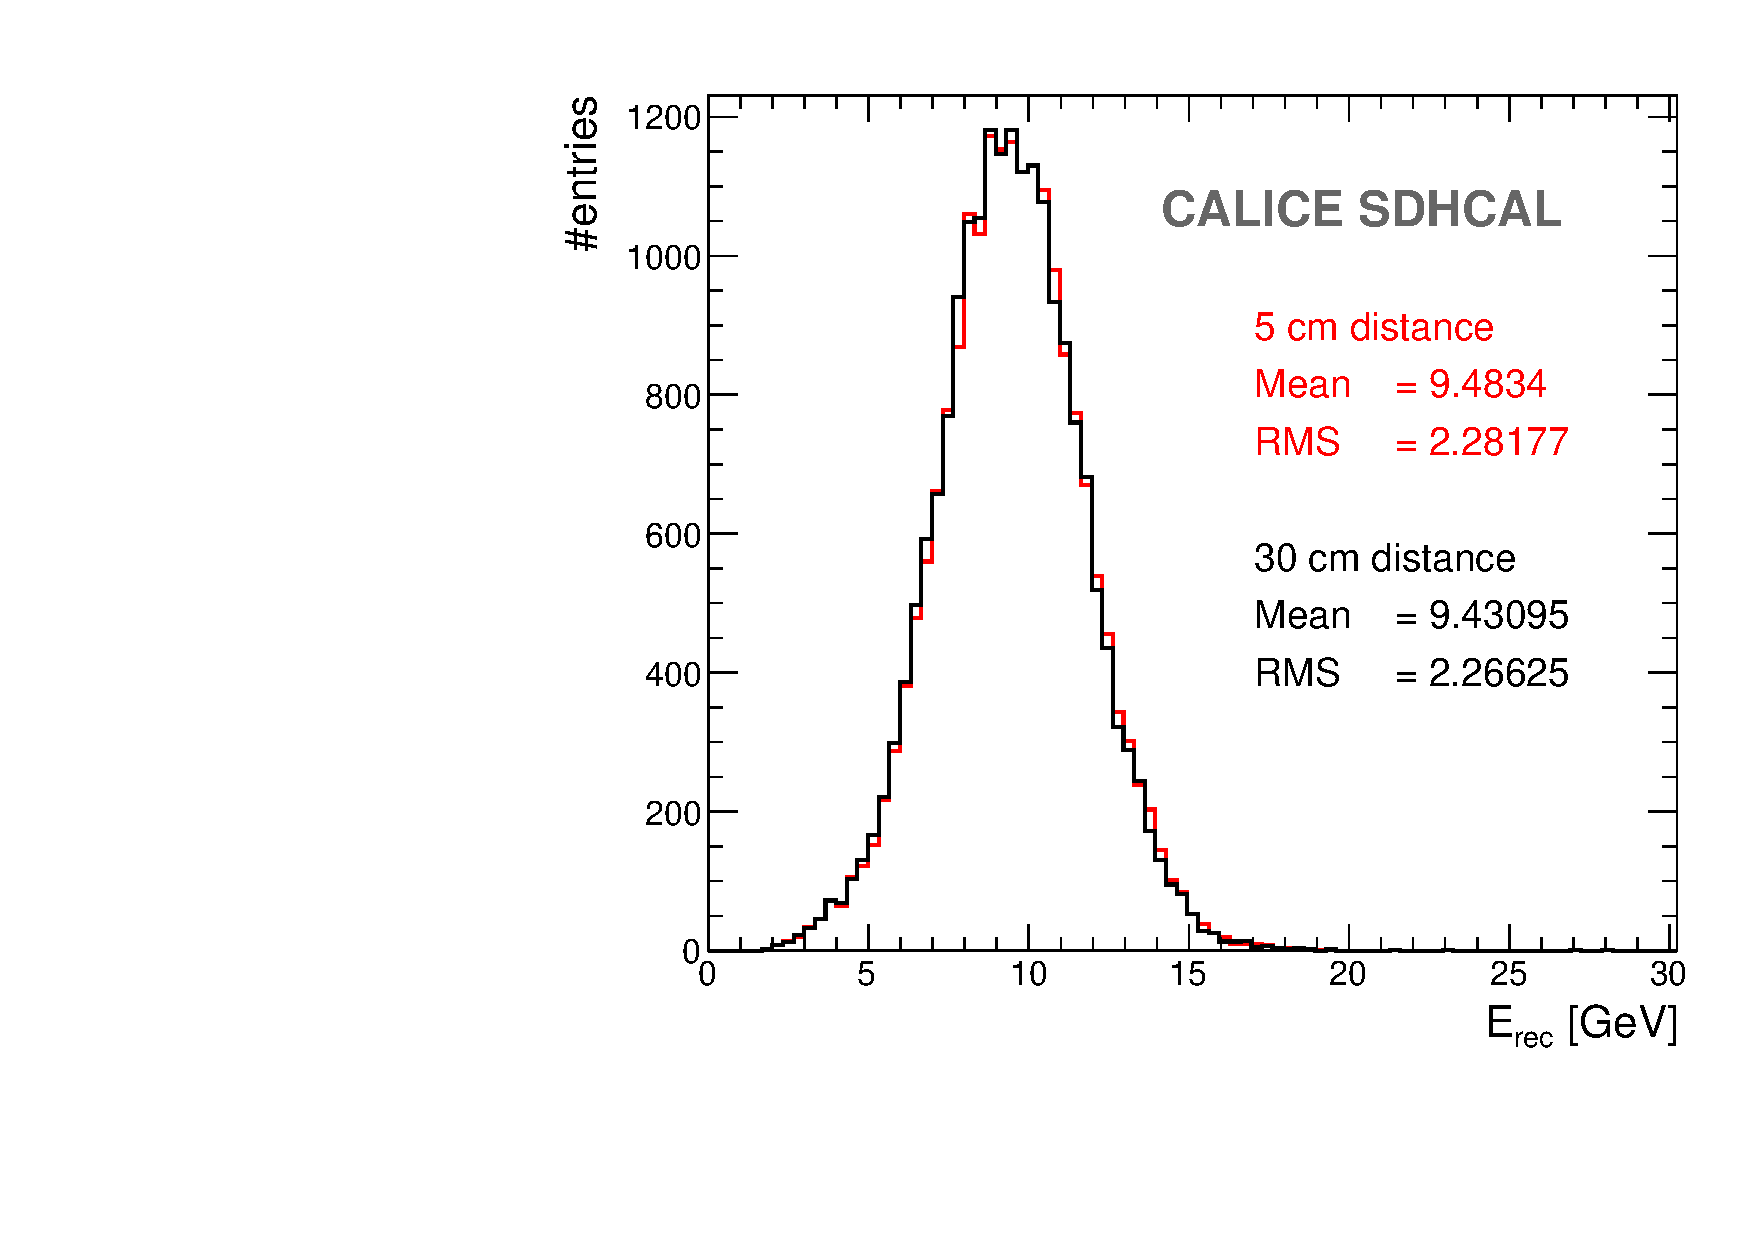
\includegraphics[width=0.45\linewidth]{plots/OverlayEvent/OverlayEvent_OverlayCheck_TB.pdf}
    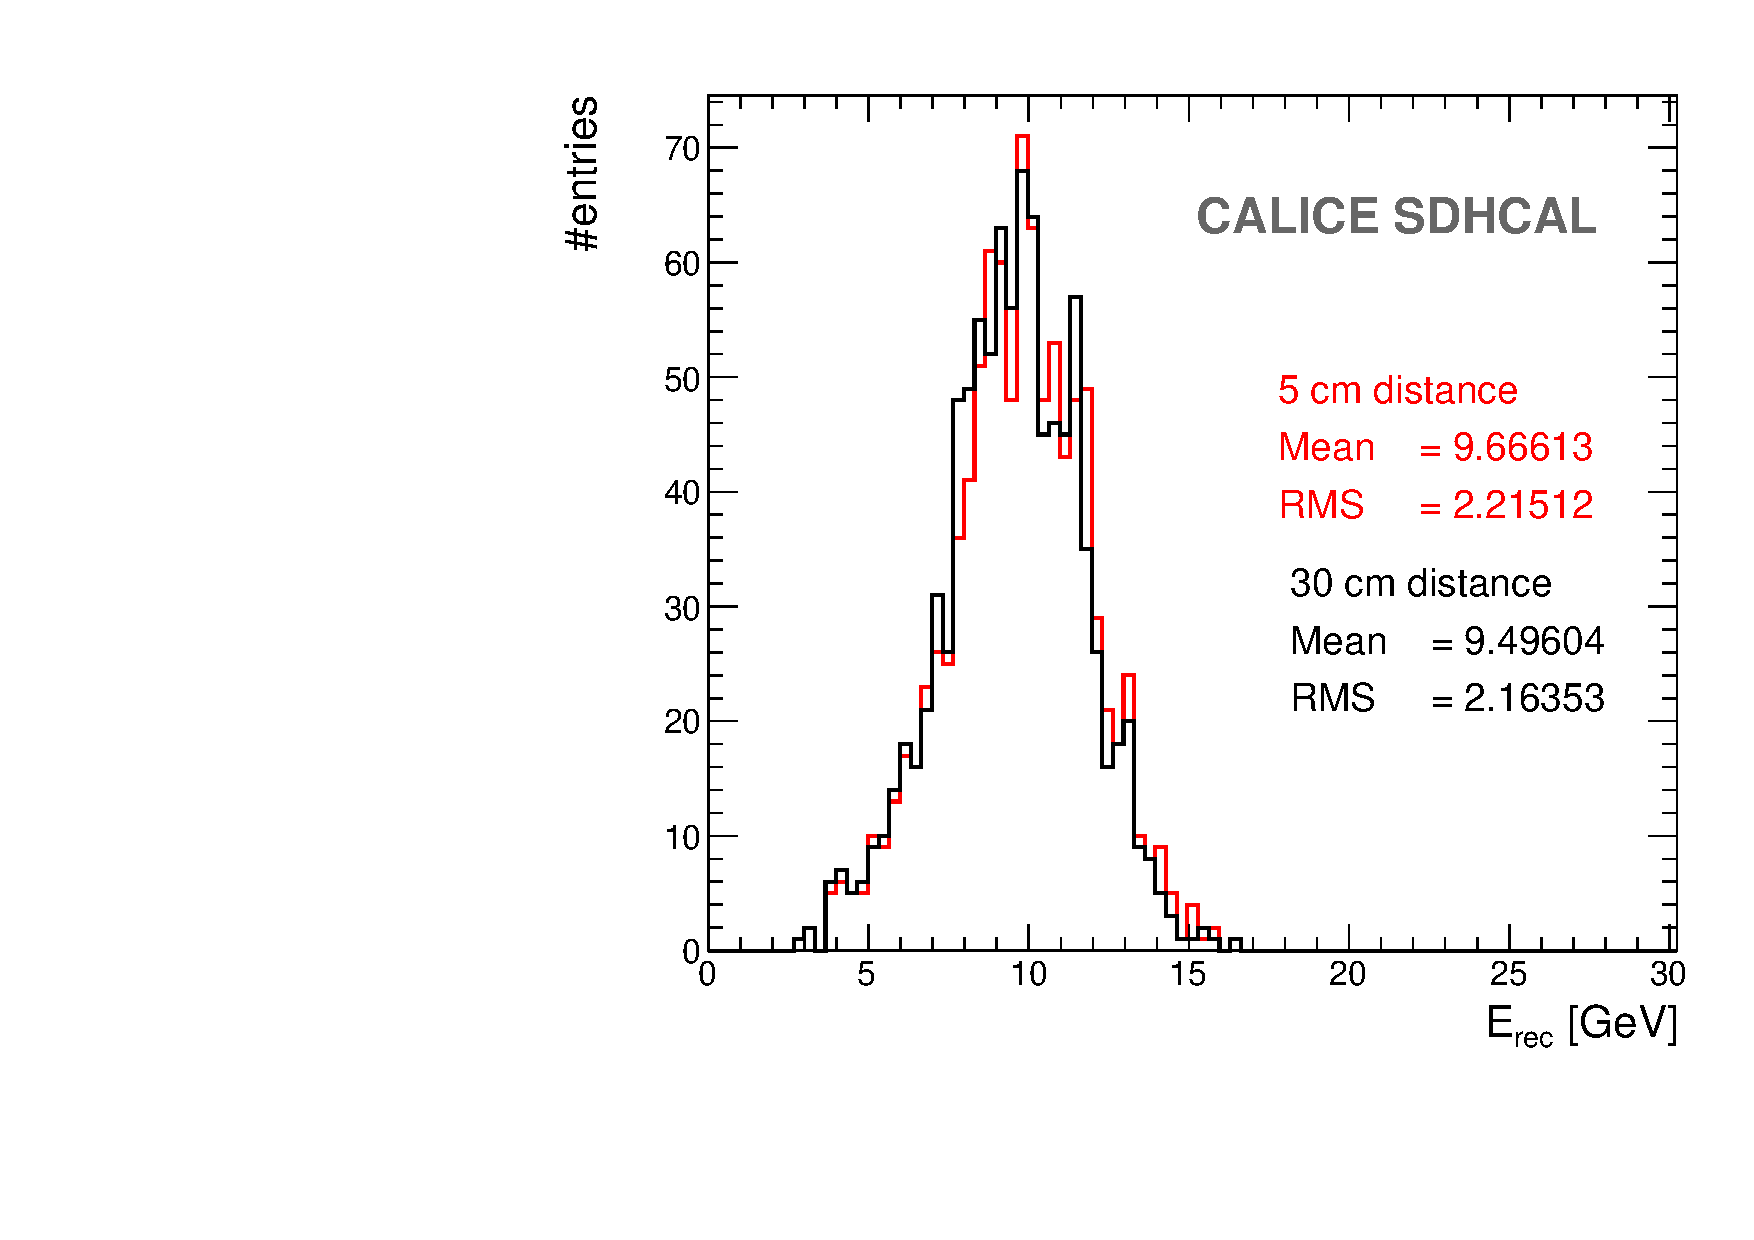
\includegraphics[width=0.45\linewidth]{plots/OverlayEvent/OverlayEvent_OverlayCheck_FTF_BIC.pdf}
    %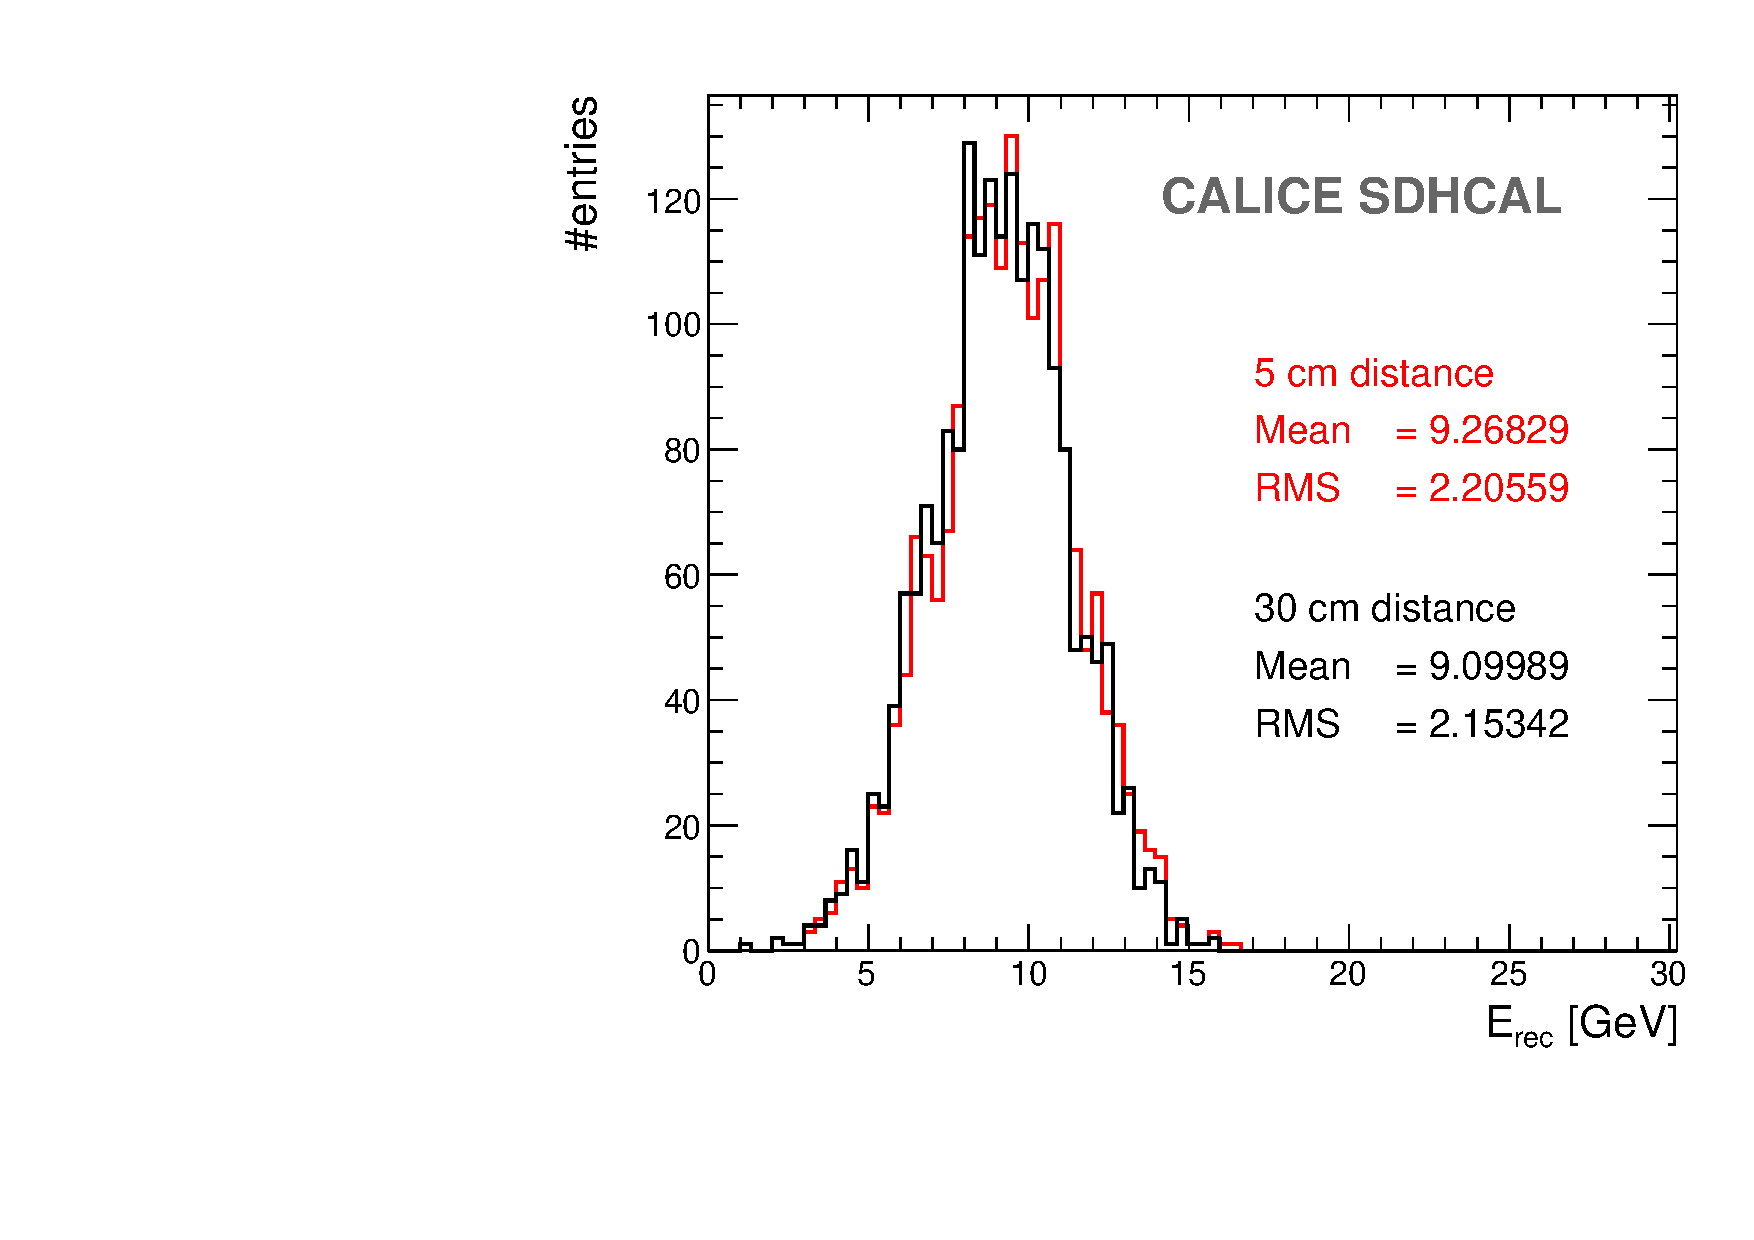
\includegraphics[width=0.32\linewidth]{plots/OverlayEvent/OverlayEvent_OverlayCheck_FTFP_BERT_HP.pdf}
  \end{center}
  \caption{\label{OVERLAY_EVENT_MC_EREC_OVERLAID_HITS} The reconstructed energy of the 10 GeV neutral hadron after the overlay procedure with a 30 GeV charged hadron with a separation distance of 30 cm (black) and 5 cm (red) for different data samples : test beam data (left) and FTF\_BIC simulation (right)}
\end{figure}

\begin{figure}[!h]
  \begin{center}
    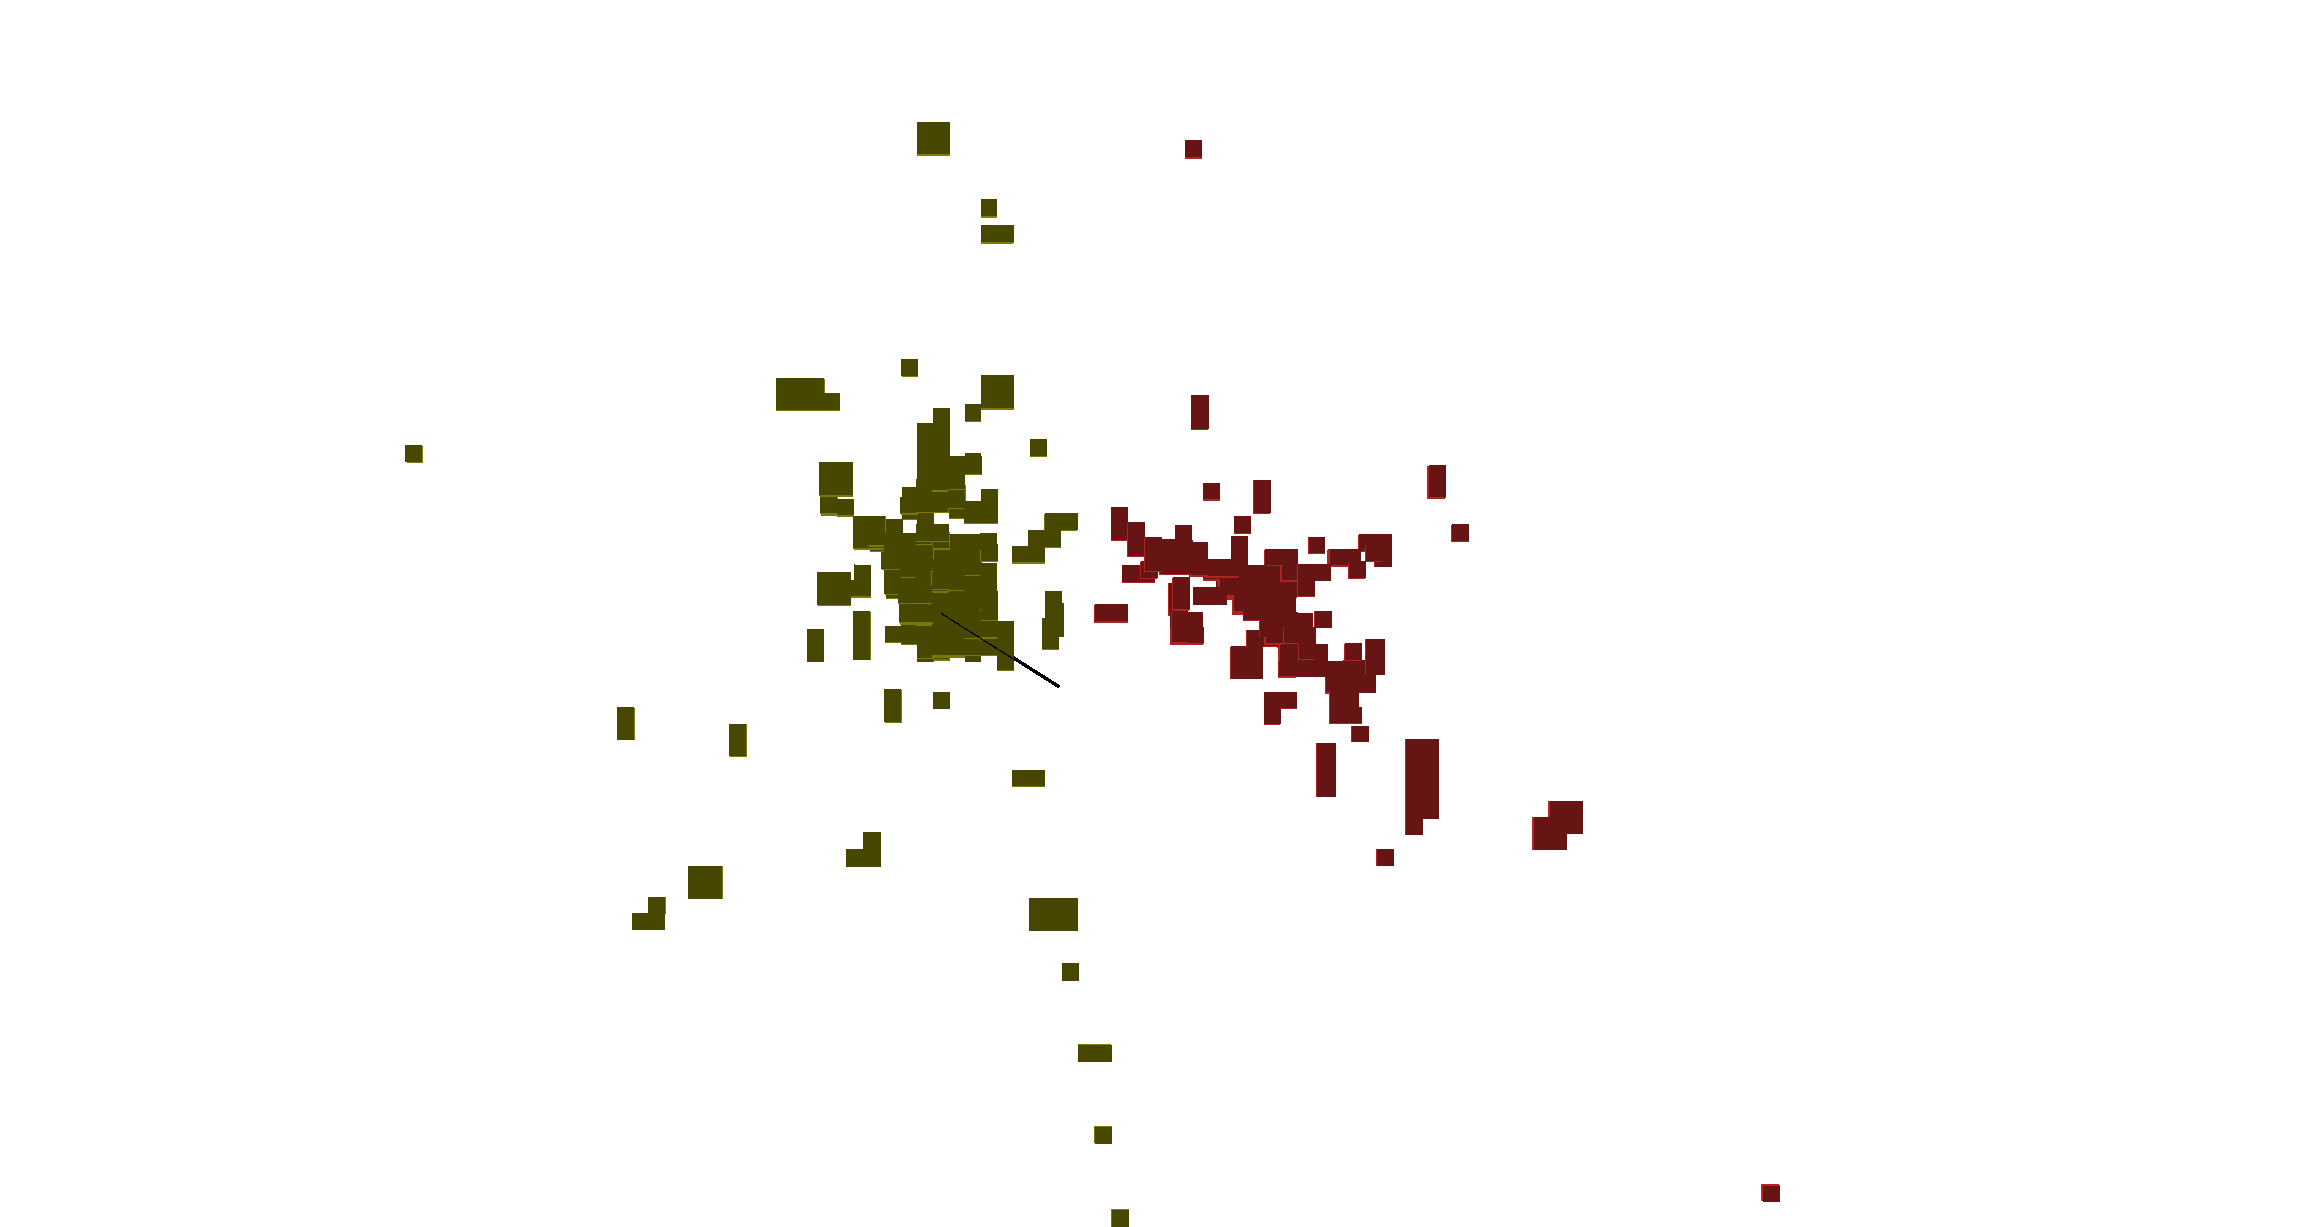
\includegraphics[width=0.28\linewidth]{ArborPFA_PandoraMonitoring_SDHCAL_Overlay_XY.pdf}
    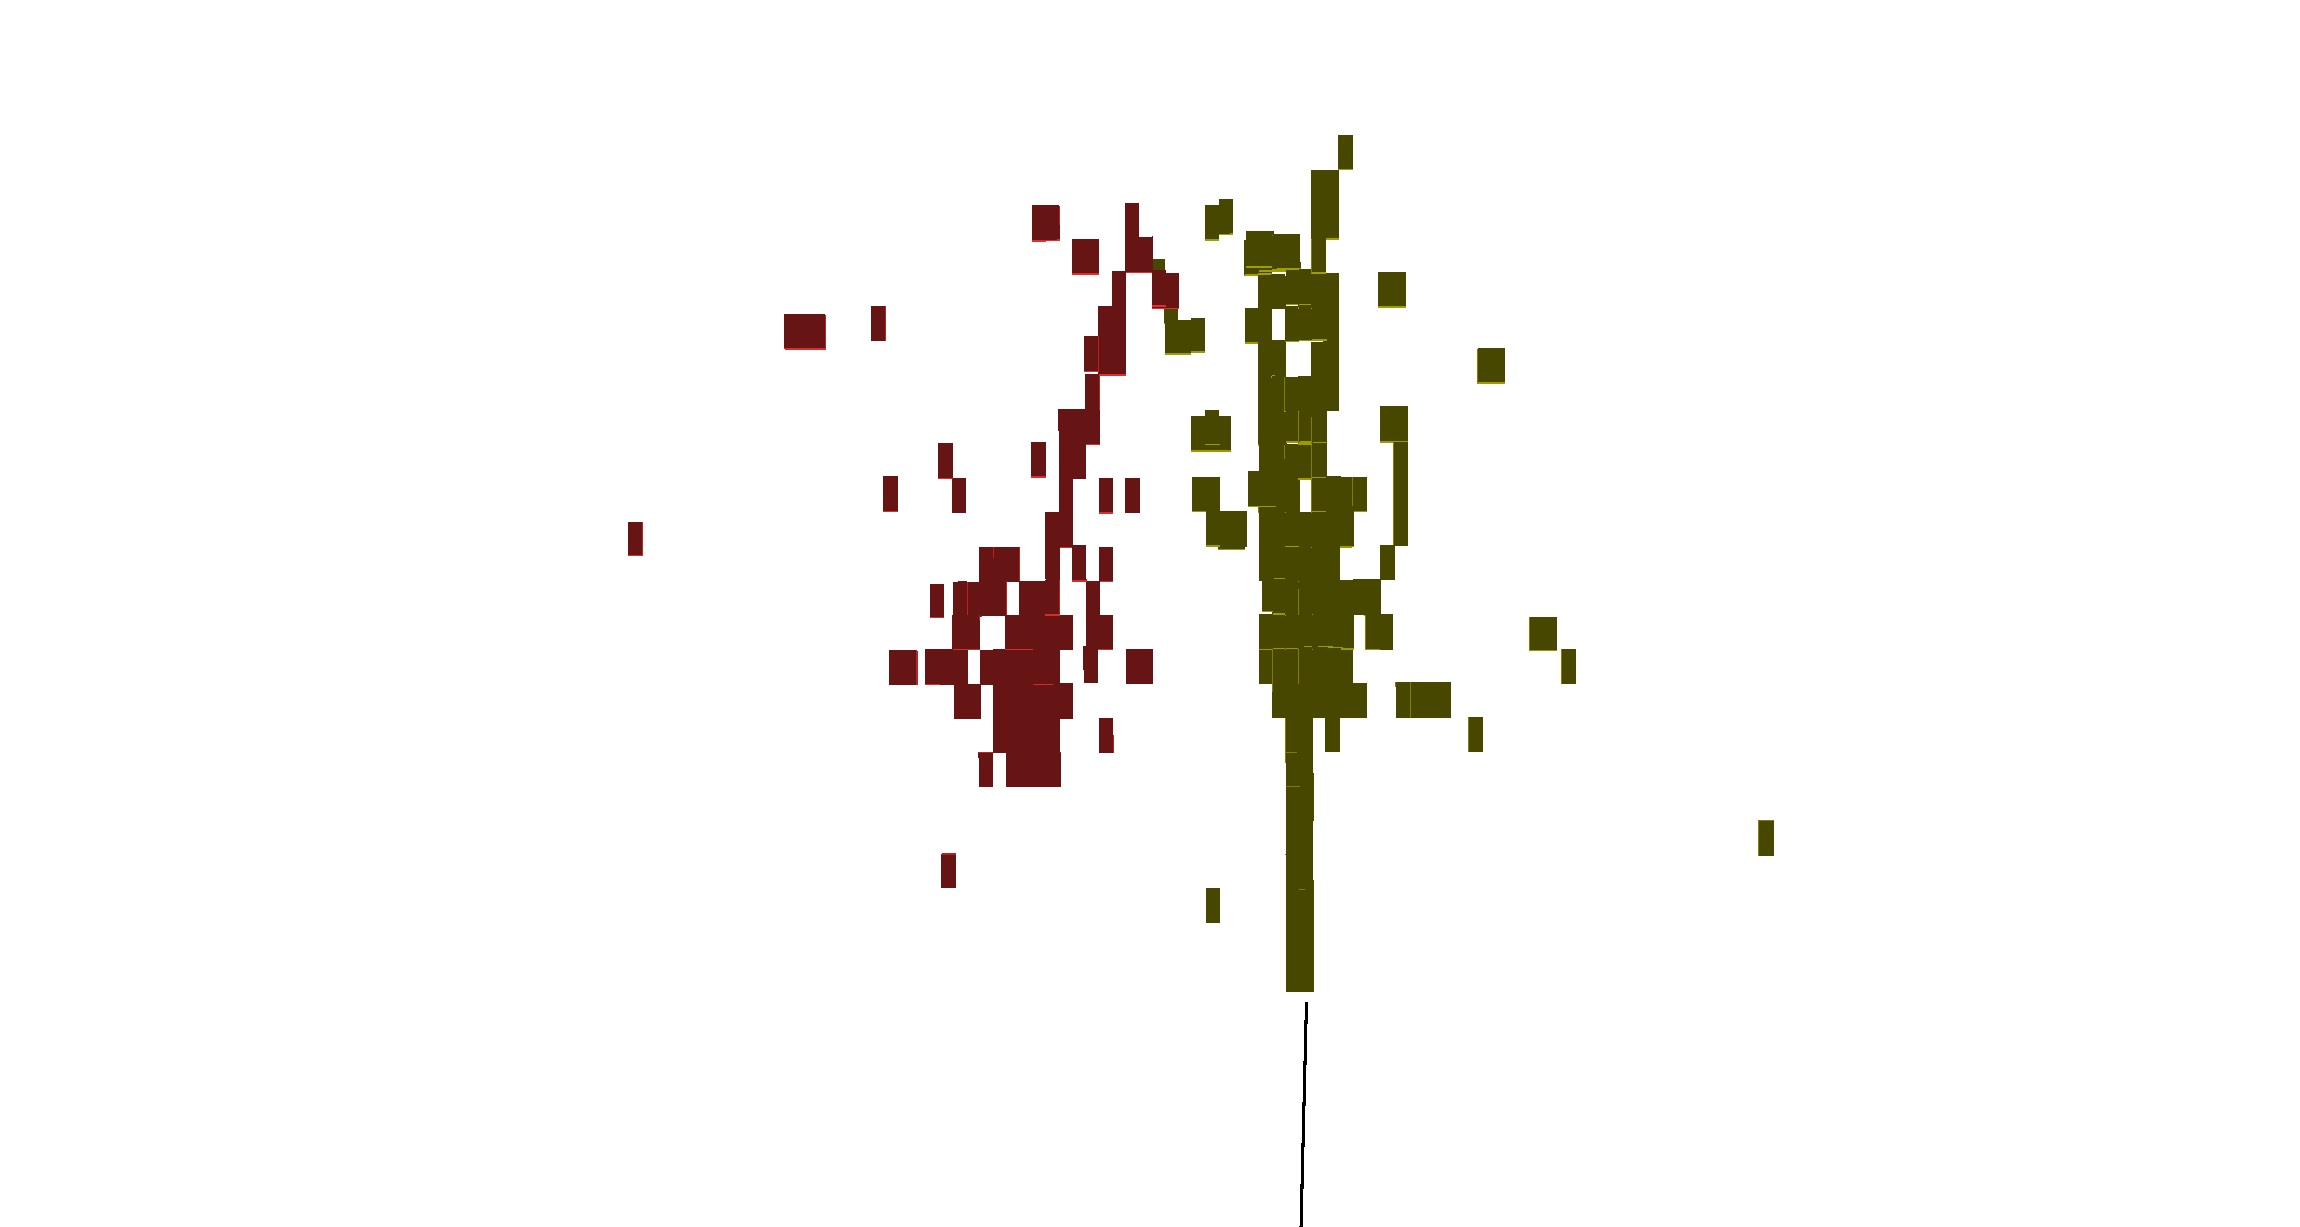
\includegraphics[width=0.28\linewidth]{ArborPFA_PandoraMonitoring_SDHCAL_Overlay_XZ.pdf}
    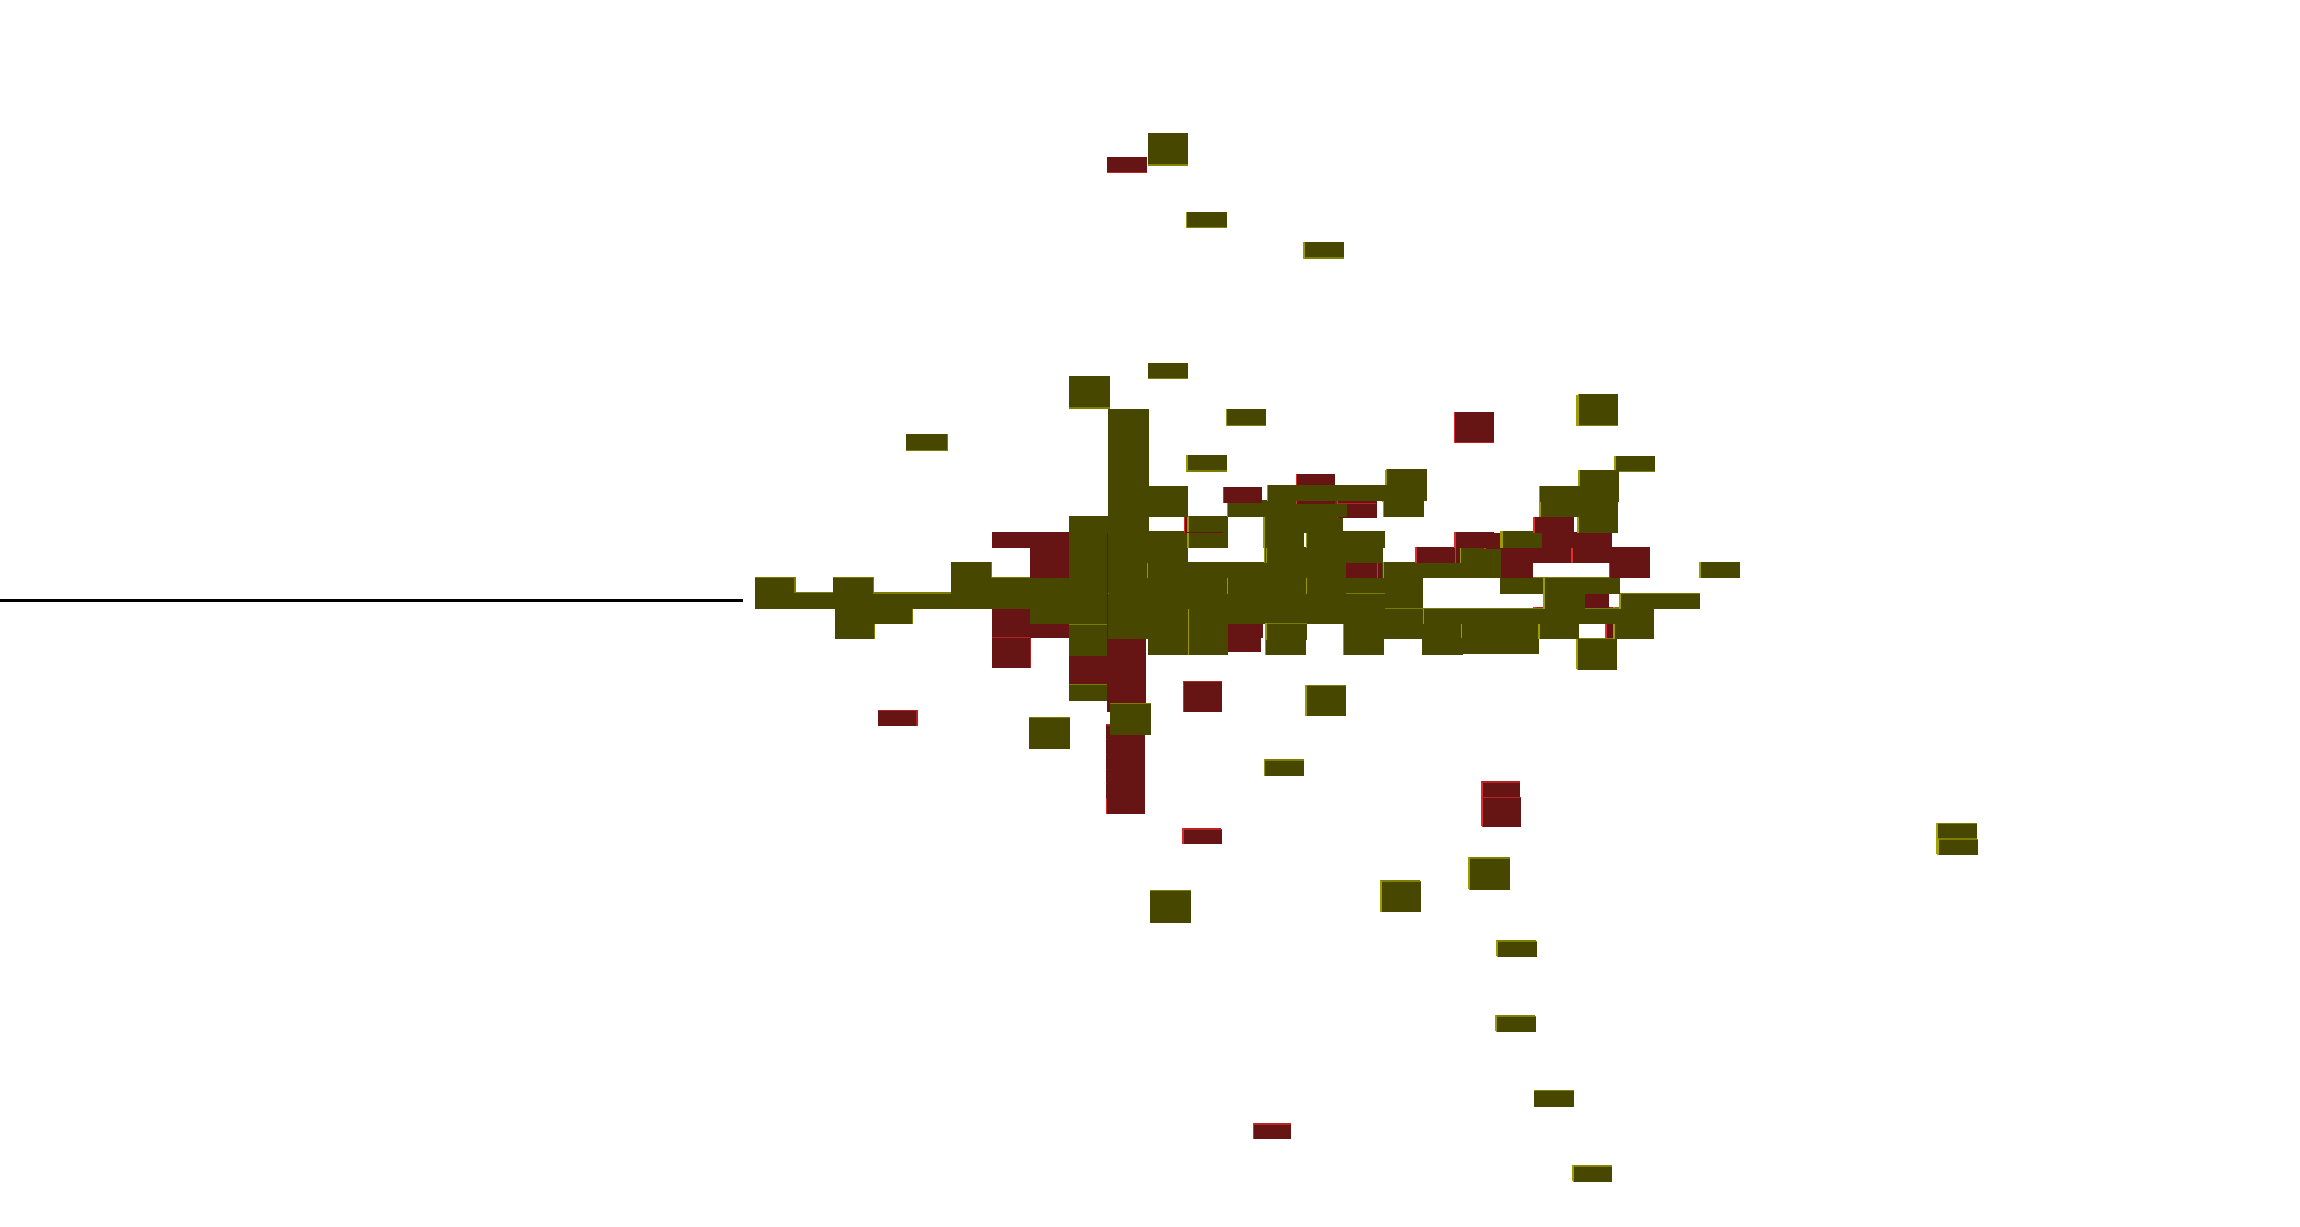
\includegraphics[width=0.28\linewidth]{ArborPFA_PandoraMonitoring_SDHCAL_Overlay_YZ.pdf}
  \end{center}
  \caption{\label{OVERLAY_EVENT_DISPLAY} 
  Display of a 10 GeV fake neutral hadron overlaid with a 30 GeV charged hadron separated by 20 cm in three different views : XoY (left), XoZ (middle) and YoZ (right). Colours correspond to the reconstructed PFOs after running the ArborPFA program. %The black straight line is the fake track generated in front of the calorimeter.
  }
\end{figure}

Figure \ref{OVERLAY_EVENT_MC_CH_EREC_NO_OVERLAY} shows the reconstructed energy of a 10 GeV charged hadron before the overlay procedure for different data samples. By comparing the mean energy of these distributions with the mean energy after the overlay at a 30 cm separation distance (Figure \ref{OVERLAY_EVENT_MC_EREC_OVERLAID_HITS}), we observe a small energy decrease of about 0.7 GeV due to the track segment hits removal while overlaying the two showers.

%A small energy difference is observed between the reconstructed energy before the overlay and after the overlay (right) for the 30 cm case (black), due to the track segment hits removal while overlaying the two showers.

%%%%%%%%%%%%%%%%%%%%%%%%%%%%%%%%%%%%%%%%%%%
%%%%%%%%%%%%%%%%%%%%%%%%%%%%%%%%%%%%%%%%%%%
\subsection{Overlaid particles analysis}

\begin{figure}[!h]
  \begin{center}
    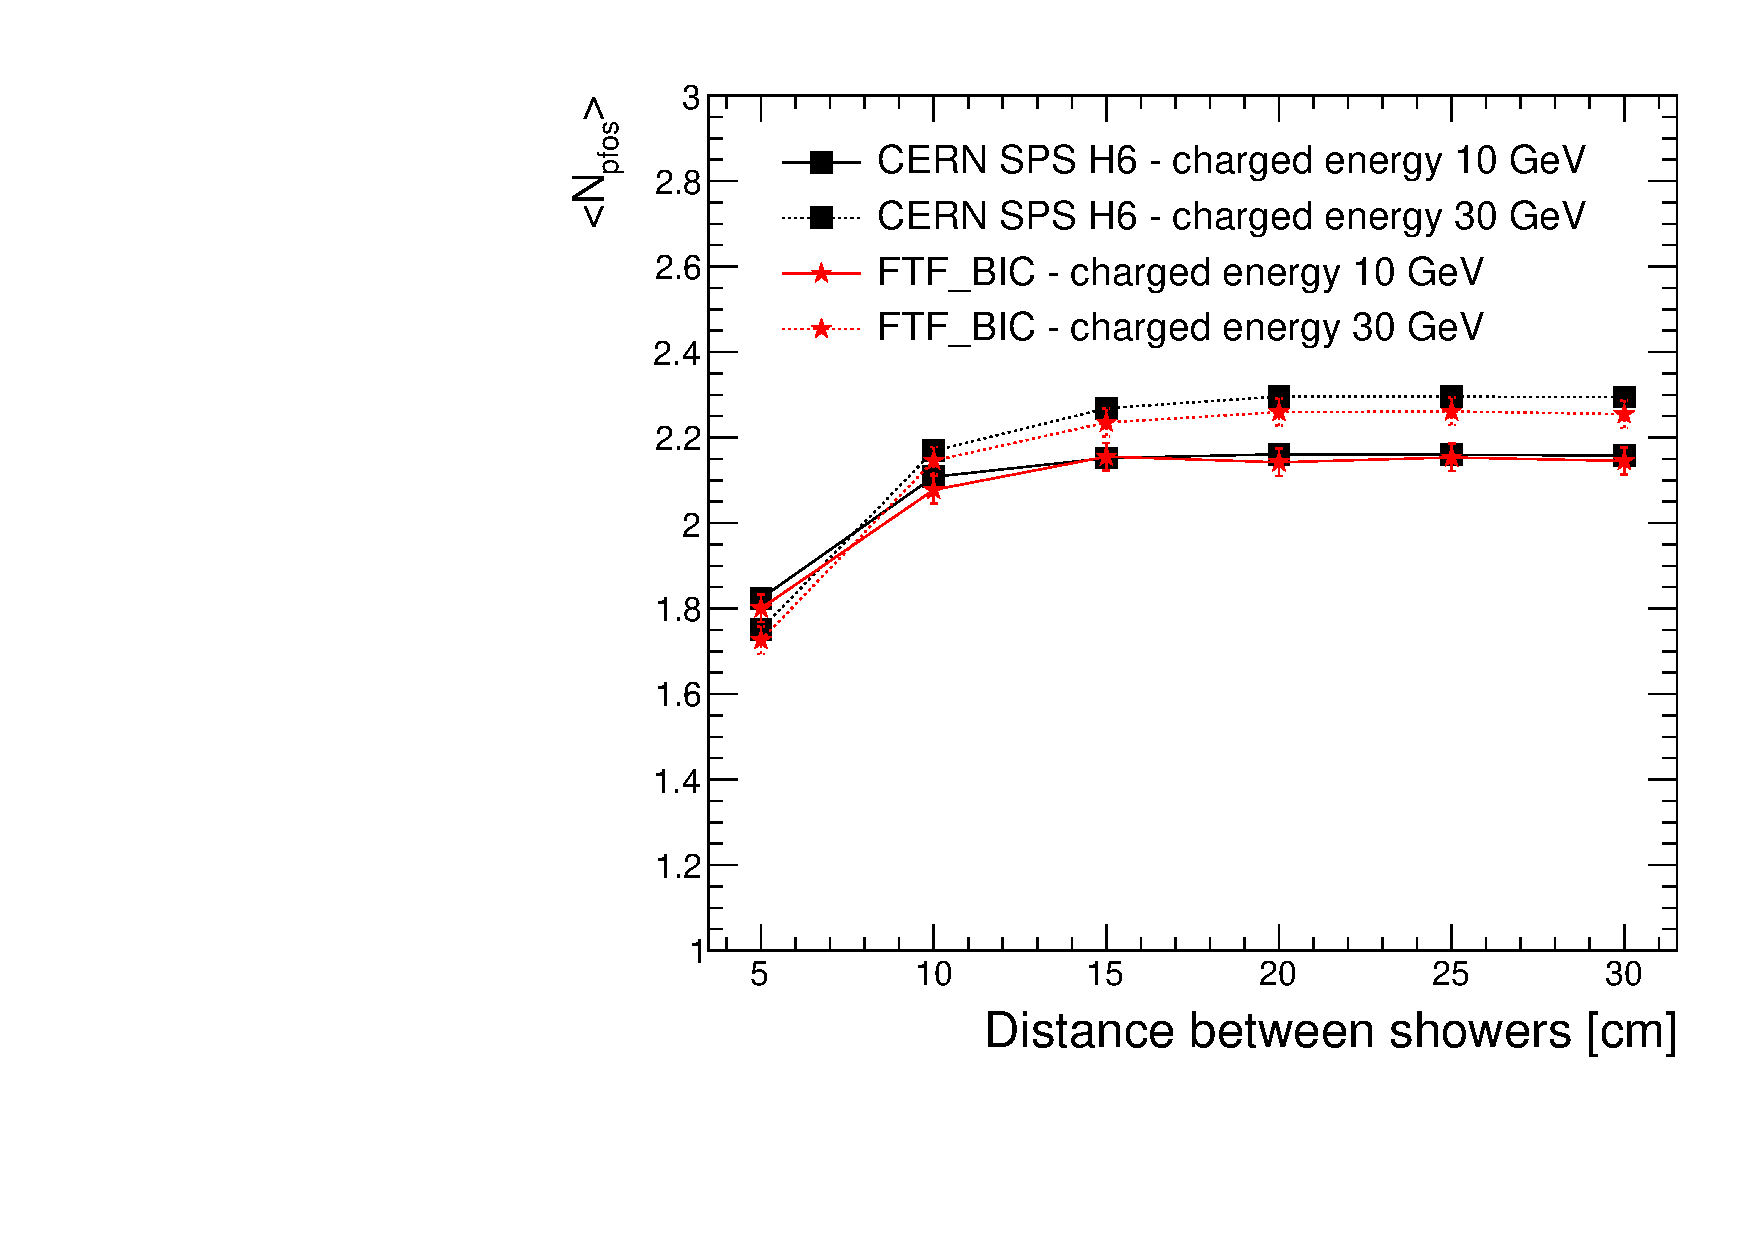
\includegraphics[width=0.6\linewidth]{plots/OverlayEvent/OverlayEvent_NPfos.pdf}
  \end{center}
  \caption{\label{OVERLAY_EVENT_NPFOS} The mean number of PFOs after running the ArborPFA program on overlaid 10 GeV emulated neutral hadron and charged hadrons at different energies.}
\end{figure}


Figure \ref{OVERLAY_EVENT_NPFOS} shows the mean number of PFOs after running the ArborPFA program on a 10 GeV fake neutral hadron overlaid with a charged hadron at different energies and different separation distances. The behaviour at large separation distance with the charged particle energy matches the mean number of PFOs of the single particle study. We can also see that the sum of the mean number of PFOs for the single particle is compatible with the mean number of PFOs for the overlay. The mean number of PFOs is stable at large separation distances but slightly decreases at 5 cm from about 2.1 PFOs down to about 1.8 PFOs due to the showers overlaps and the resulting confusion.

\begin{figure}[!h]
  \begin{center}
    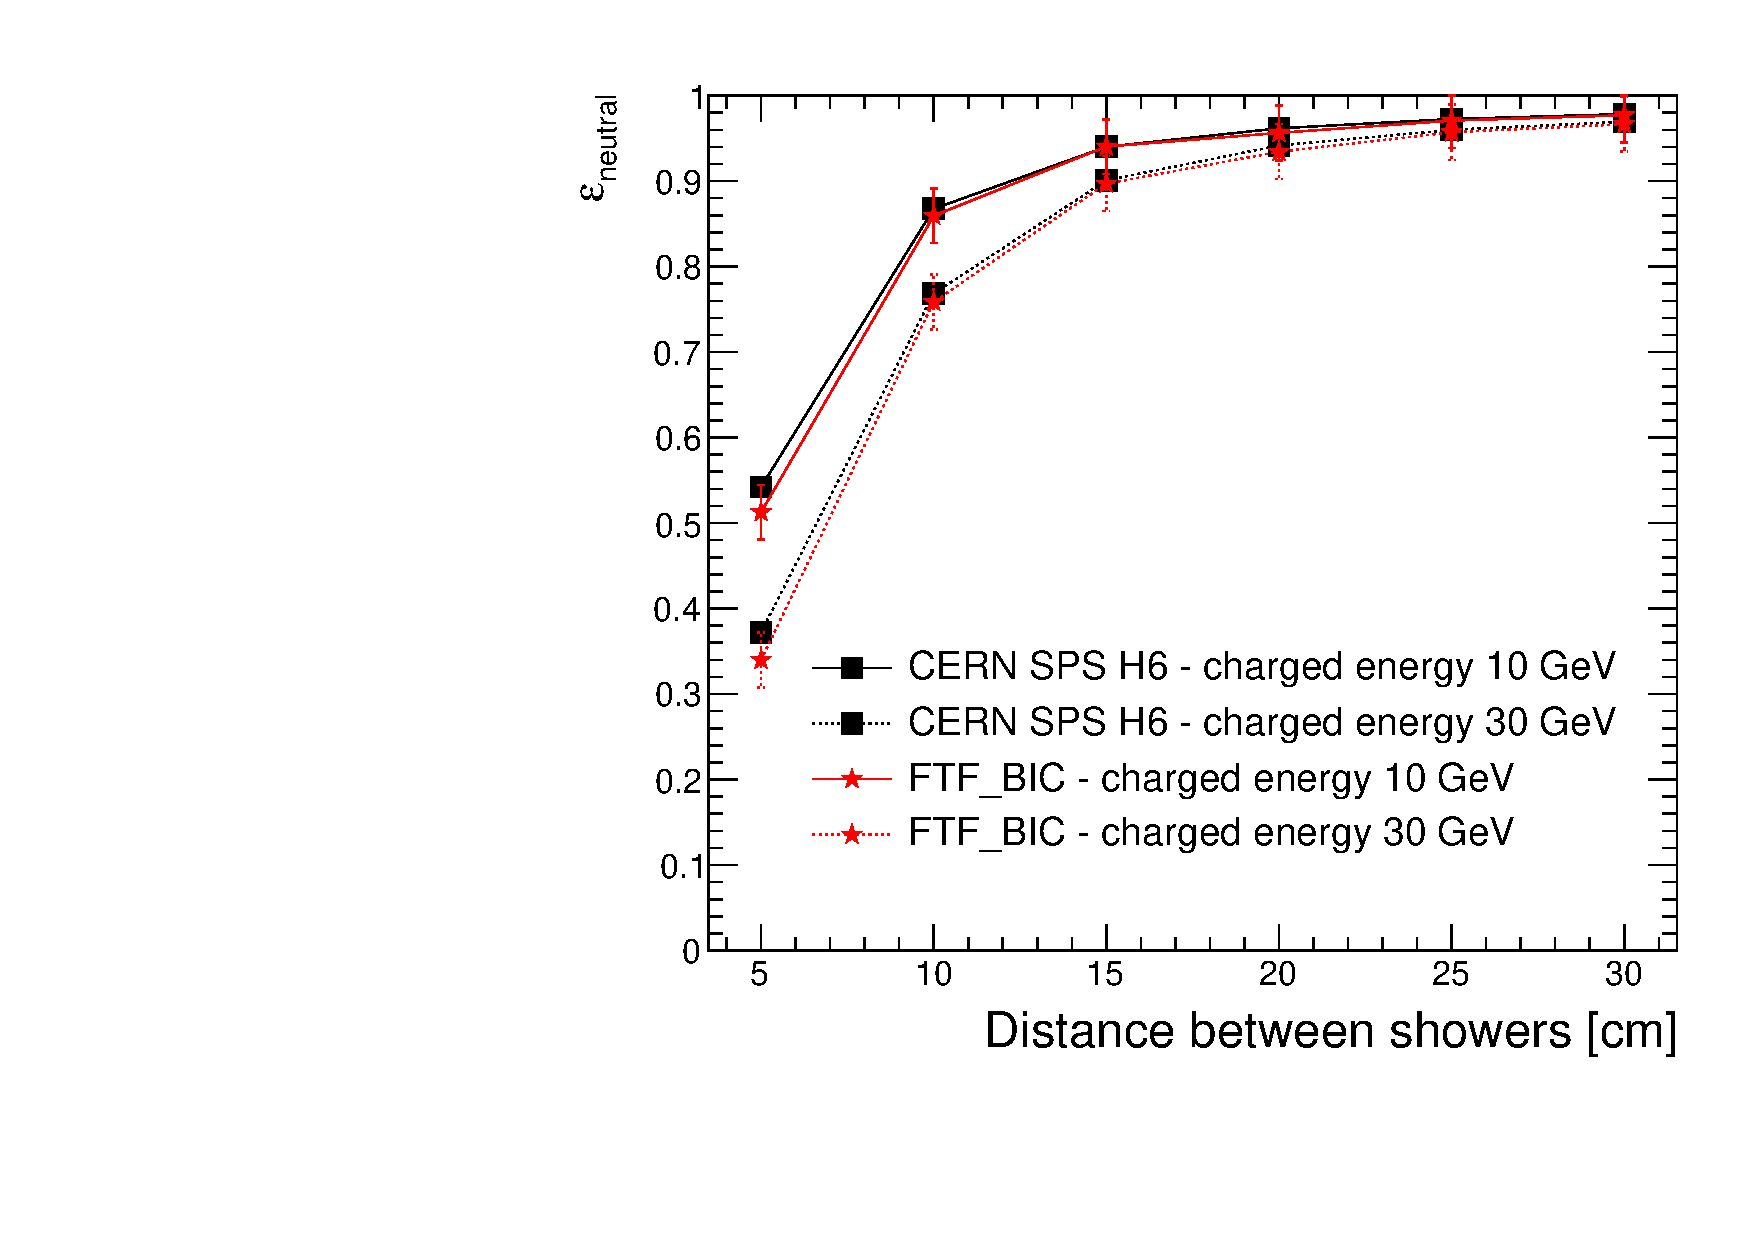
\includegraphics[width=0.47\linewidth]{plots/OverlayEvent/OverlayEvent_Efficiency.pdf}
    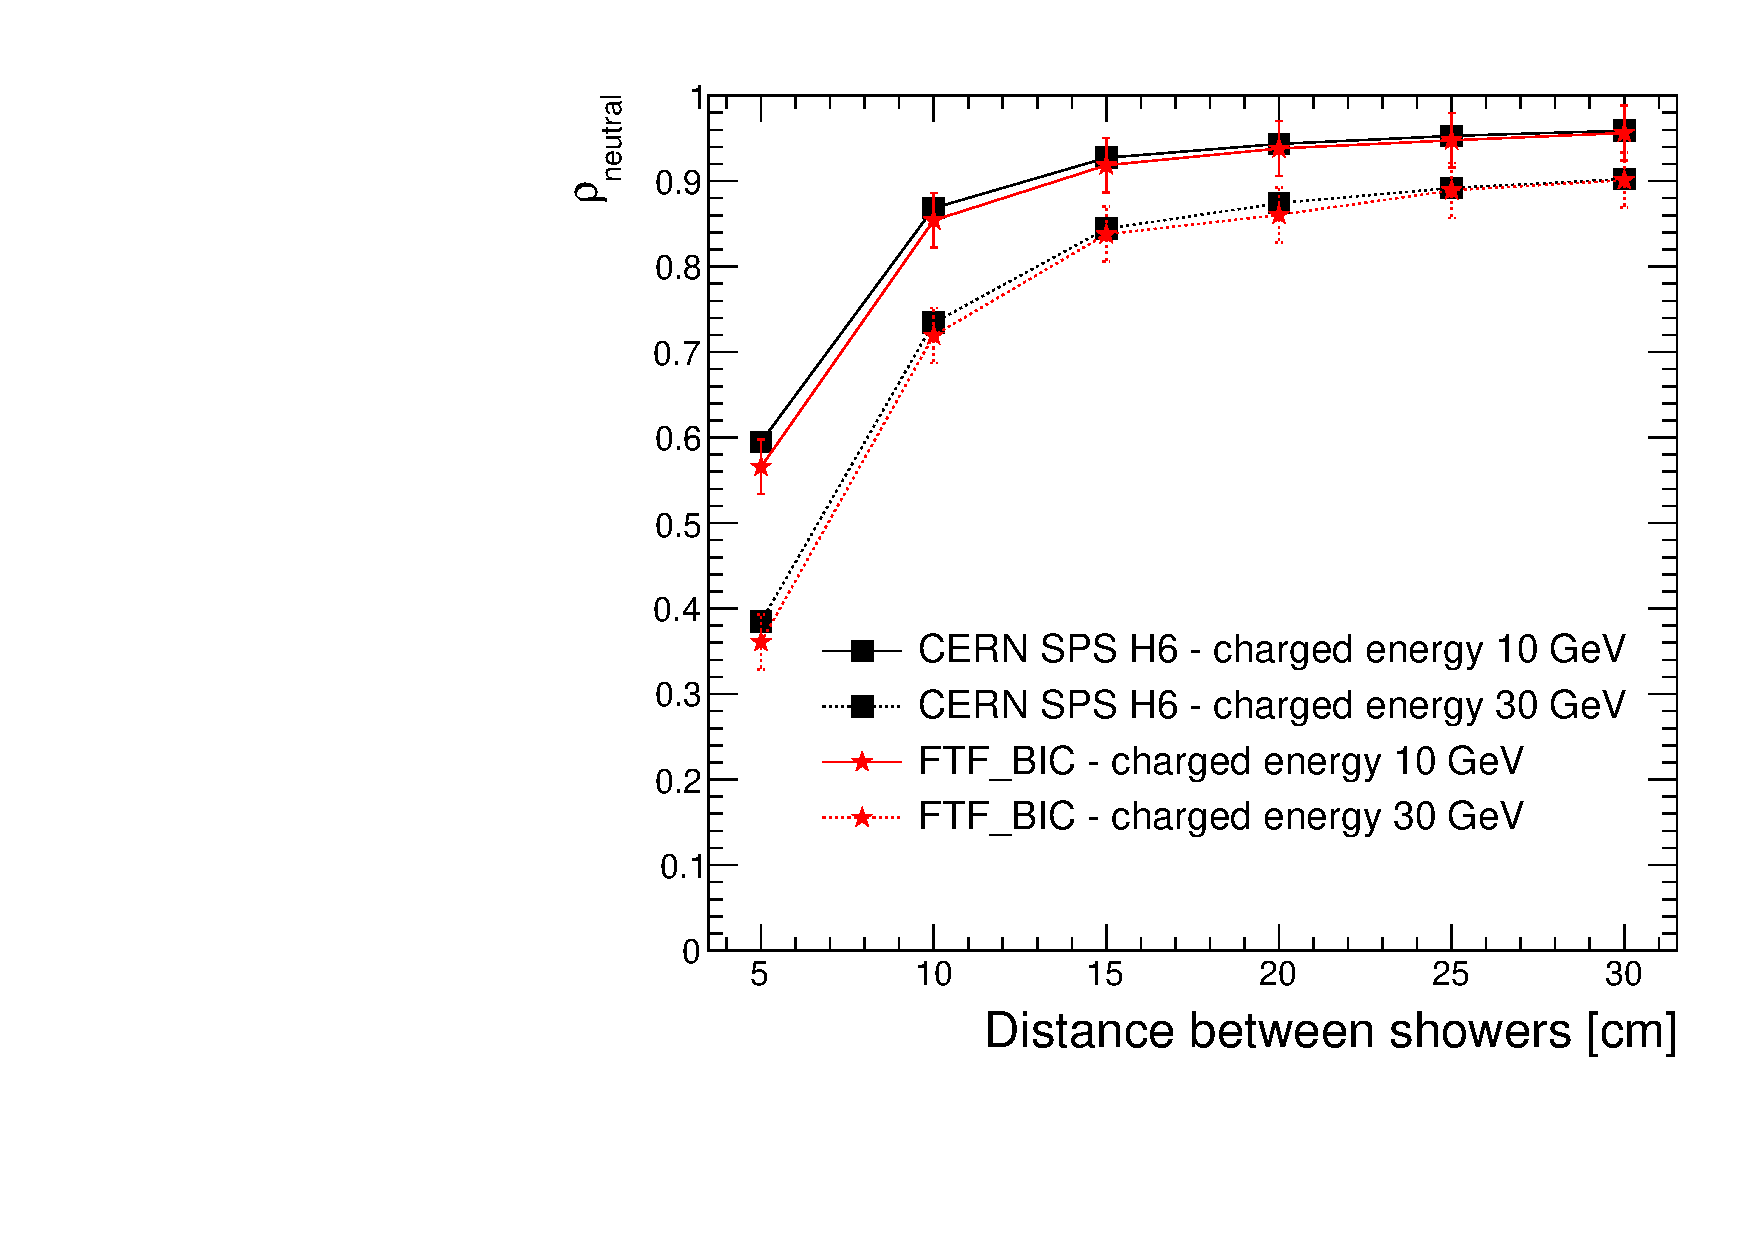
\includegraphics[width=0.47\linewidth]{plots/OverlayEvent/OverlayEvent_Purity.pdf}
  \end{center}
  \caption{\label{OVERLAY_EVENT_PURITY_EFFICIENCY} The efficiency (left) and purity (right) of the 10 GeV neutral hadron after reconstruction.}
\end{figure}


To quantify the separation, we define the efficiency and the purity related to the reconstruction of one of the two related showers as :

\begin{equation}
  \epsilon = \frac{Nhit_{good}}{Nhit_{ini,tot}}
\end{equation}
\begin{equation}
  \rho = \frac{Nhit_{good}}{Nhit_{rec,tot}}
\end{equation}

with Nhit$_{good}$ the number of hits that initially belongs to the particle and correctly assigned after reconstruction, Nhit$_{rec,tot}$ the total number of hits of the reconstructed shower and Nhit$_{ini,tot}$ the total number of hits of the particle before reconstruction. 

Figure \ref{OVERLAY_EVENT_PURITY_EFFICIENCY} shows the efficiency (left) and the purity (right) of the neutral hadron for different charged particle energies and different separation distances. In the same way as for the mean number of PFOs, at small distances the two showers start to overlap and confusions appear in the reconstruction. Thus, some hits of the neutral hadron are assigned to the charged one (and vice versa) and the efficiency and purity decrease. At large separation distances, the purity does not tend to 100\%. This is due to the last performed algorithm (small neutral fragment algorithm) which merges small neutral cluster fragments to their closest parent cluster, without considering the parent cluster size or energy. Since the number of neutral fragments for a single hadron particle increases with the energy, a non-negligible part of the charged hits is assigned to the neutral hadron, leading to a decrease of its purity.

Figure \ref{OVERLAY_EVENT_NEUTRAL_PERCENTAGE} (left) shows the fraction of events in which at least one neutral hadron has been reconstructed. As expected, the number of reconstructed neutral particles decreases with the separation distance. From 30 cm down to 15 cm, this fraction is stable and greater than 97\%. At 10 cm, confusion becomes significant and the neutral hadron is sometimes merged with the charged one, leading to a small decrease of this fraction. At 5 cm, we can see that the fraction strongly depends on the charged particle energy and goes from 73\% of reconstructed events for the 10 GeV charged particle case down to 62\% at 30 GeV.

\begin{figure}[!h]
  \begin{center}
    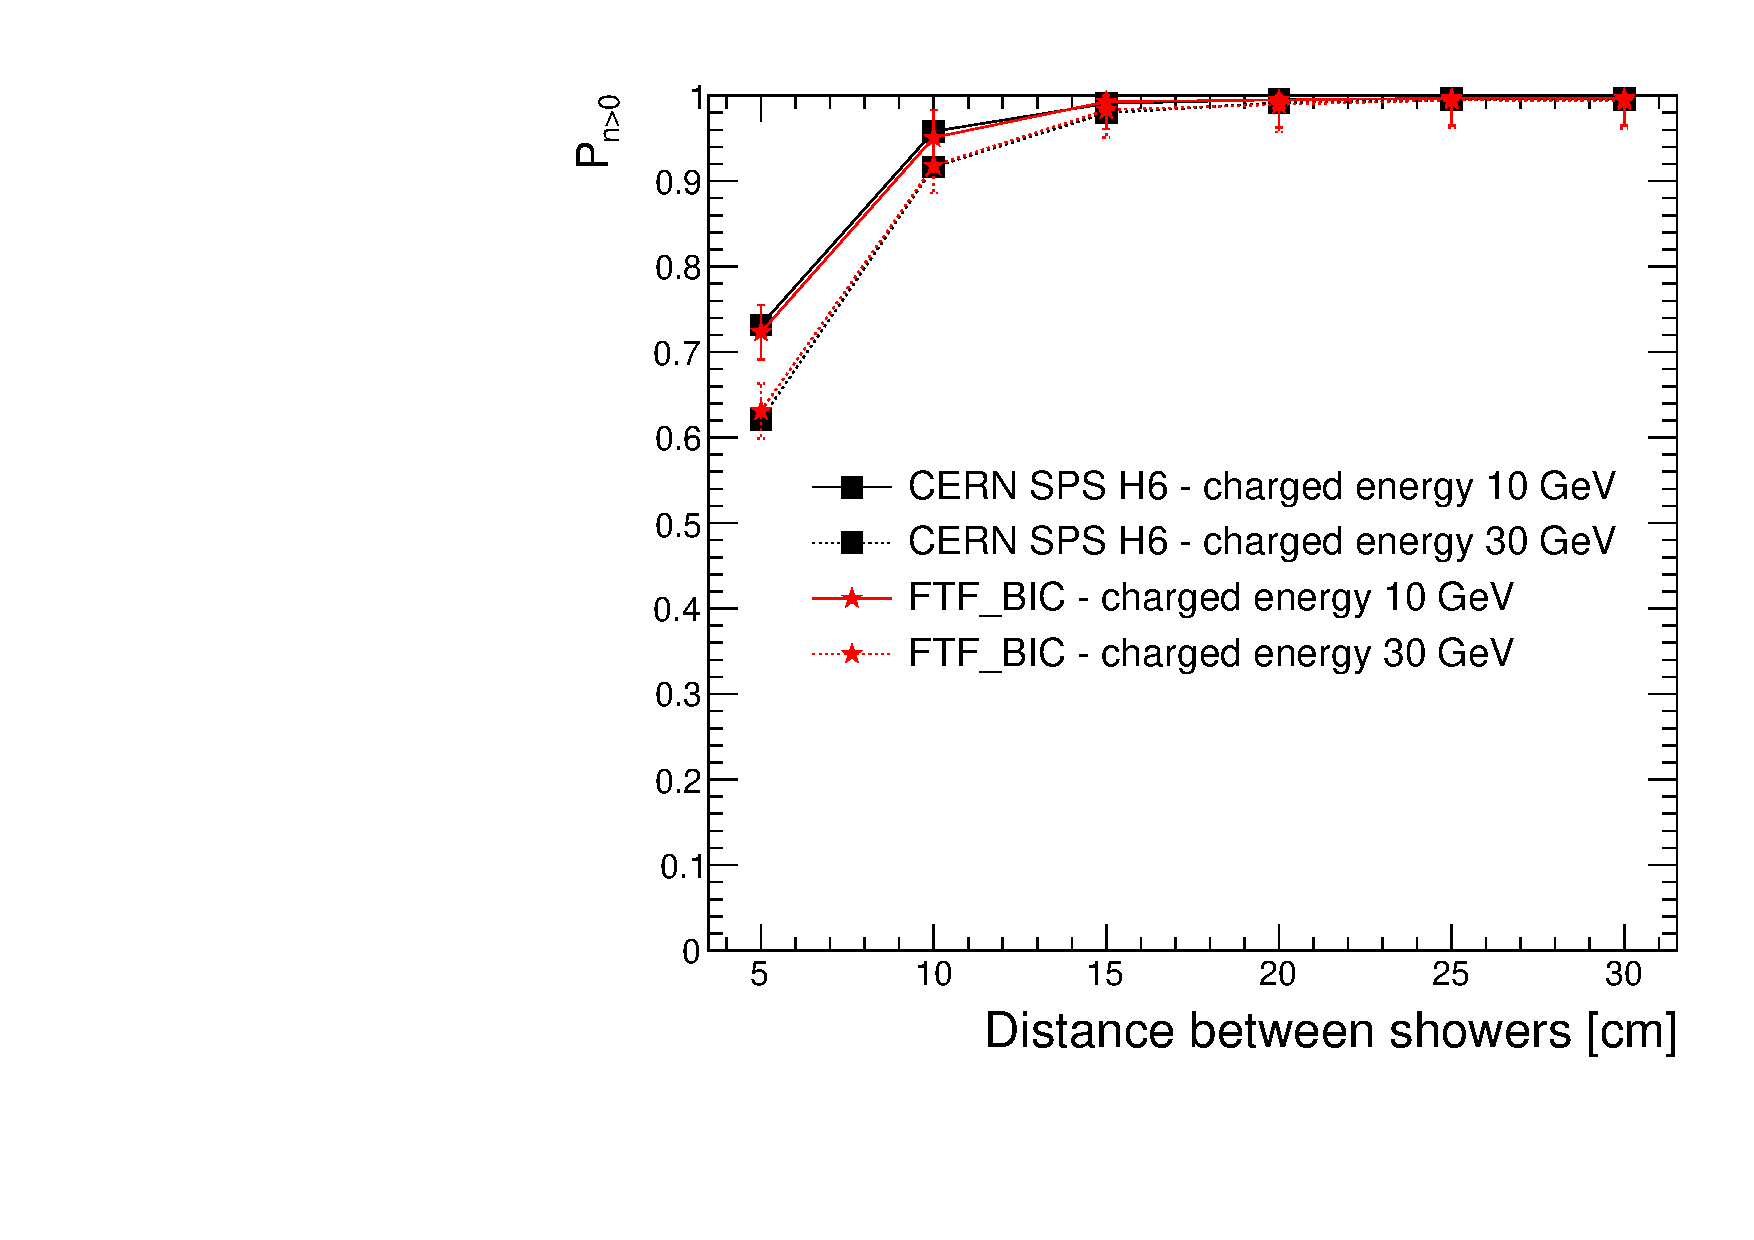
\includegraphics[width=0.47\linewidth]{plots/OverlayEvent/OverlayEvent_ProbaNeutral.pdf}
    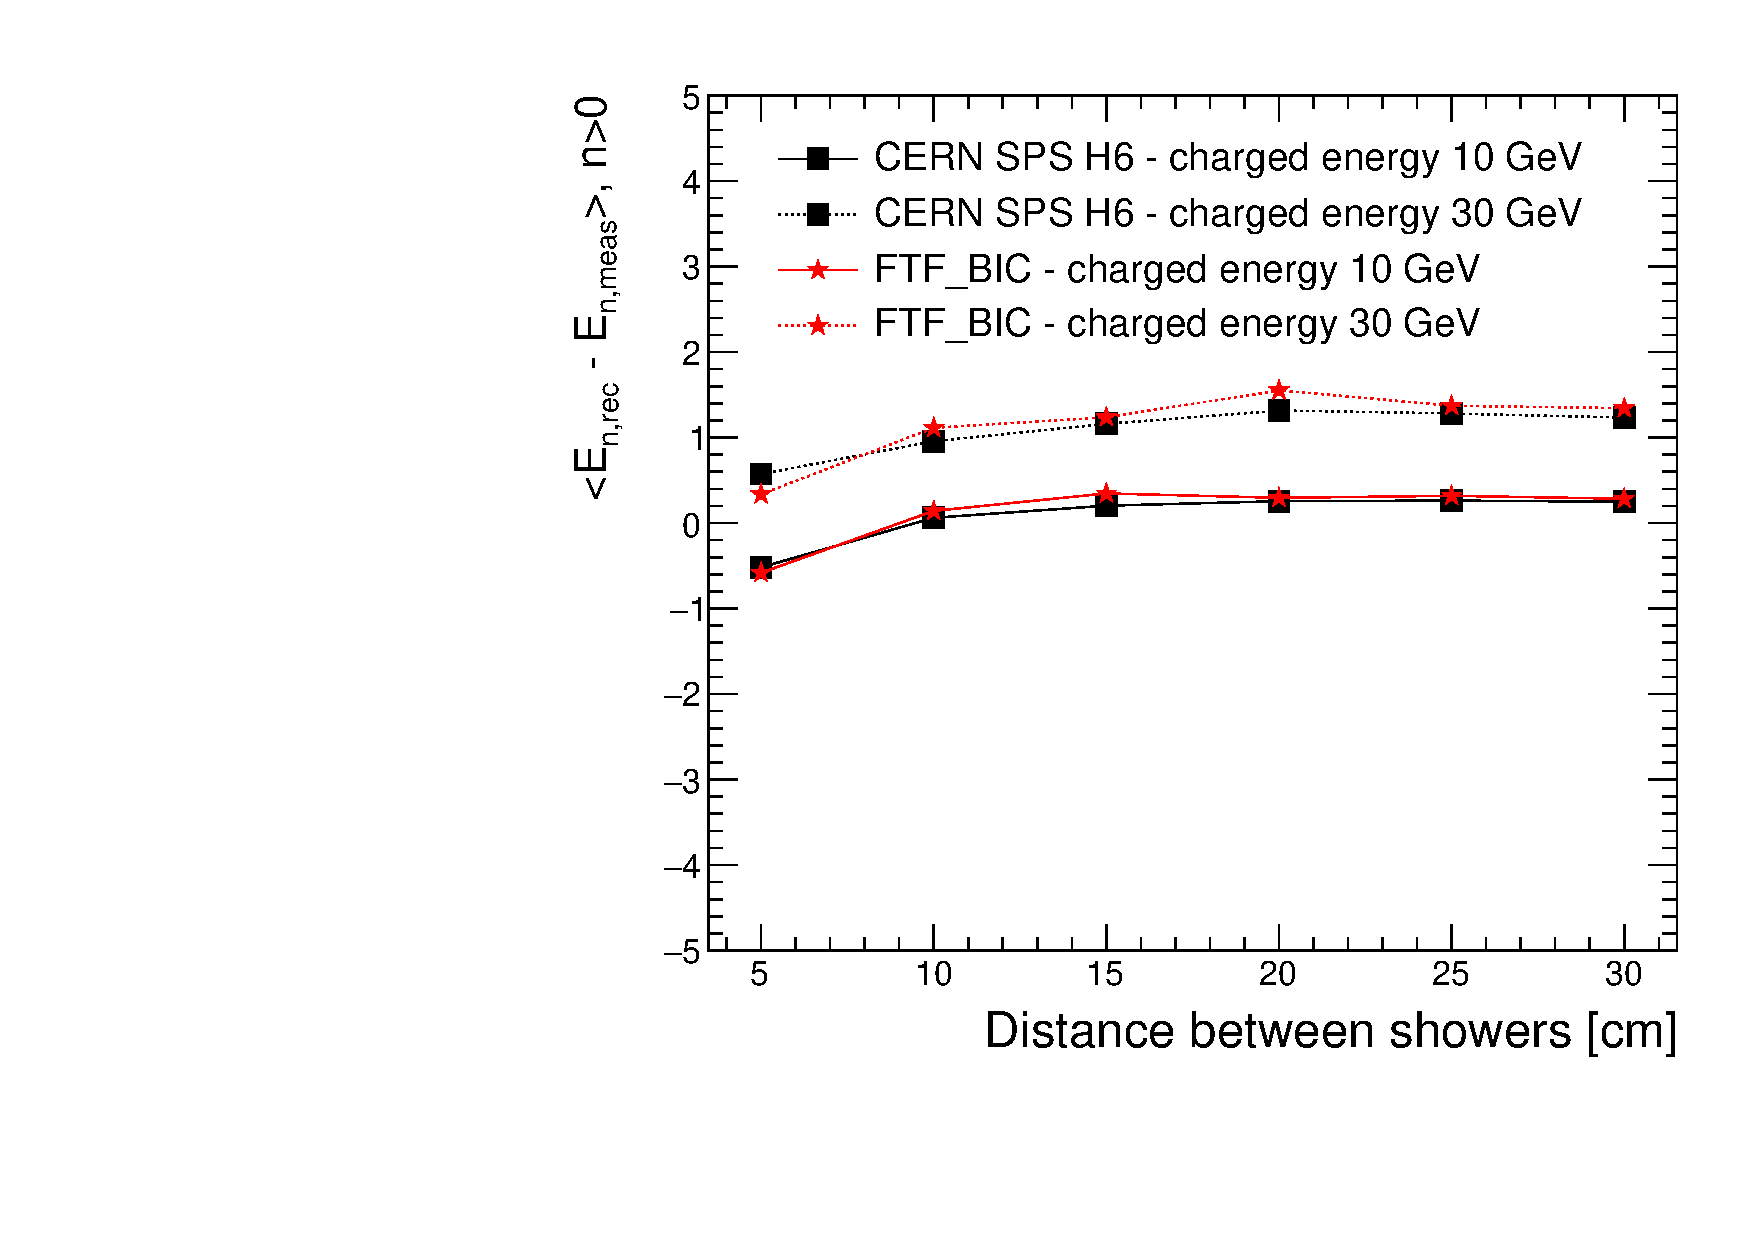
\includegraphics[width=0.47\linewidth]{plots/OverlayEvent/OverlayEvent_EnergyDifference.pdf}
  \end{center}
  \caption{\label{OVERLAY_EVENT_EREC} \label{OVERLAY_EVENT_NEUTRAL_PERCENTAGE} Left : The fraction of events where at least one neutral hadron has been reconstructed. Right : The mean difference between the reconstructed energy and the measured energy before reconstruction in events with at least one reconstructed neutral hadron.}
\end{figure}

We define the reconstructed neutral energy as the sum of the neutral particle energies and the measured neutral energy as the estimated energy before reconstruction. Figure \ref{OVERLAY_EVENT_EREC} (on the right) shows the mean difference between the reconstructed neutral energy and the measured neutral energy when at least one neutral hadron has been reconstructed. For the same reason as for the purity, the mean reconstructed neutral energy increases with the charged particle energy. This plot also shows a flat behavior of the reconstructed neutral energy with the separation distance. This means that the reconstruction of the neutral hadron at very small distance (5 cm) has a \textit{binary-like} behaviour, either well reconstructed or completely merged with the charged hadron.


%%%%%%%%%%%%%%%%%%%%%%%%%%%
%%%%%% Uncertainties %%%%%%
%%%%%%%%%%%%%%%%%%%%%%%%%%%
\clearpage
\newpage
\section{Systematic uncertainties}

For the analysis performed in section \ref{SINGLE_PARTICLE_STUDY_SECTION} and \ref{OVERLAY_EVENT_SECTION}, both statistical and systematic uncertainties are taken into account. The systematic uncertainties are estimated by varying the most important algorithm parameters. Table \ref{UNCERTAINTIES_ALGORITHM_TABLE} summarize the algorithm parameters choice, their nominal values and variations for the systematic uncertainties evaluation.

\begin{table}[!h]
  \begin{center}
     \begin{tabular}{|l|c|c|c|}
     \hline
     Parameter                  & Nominal value & Lower value & Upper value \\ \hline 
     Connection distance 1      & \textbf{45} mm   & 42.5 mm  & 47.5 mm \\ \hline
     Connection distance 2      & \textbf{65} mm   & 62.5 mm  & 67.5 mm \\ \hline
     Connection angle           & \textbf{0.7} rad & 0.65 rad & 0.75 rad \\ \hline
     Backward cleaning weight 1 & \textbf{2}       & 1.5      & 2.5  \\ \hline
     Forward  cleaning weight 1 & \textbf{3}       & 2.5      & 3.5  \\ \hline
     Backward cleaning weight 2 & \textbf{0.1}     & 0.05     & 0.15 \\ \hline
     Forward  cleaning weight 2 & \textbf{5}       & 4.5      & 5.5  \\ \hline
     Small fragment size cut    & \textbf{20}      & 19       & 21   \\ \hline
     \end{tabular}
     \caption{\label{UNCERTAINTIES_ALGORITHM_TABLE} Algorithm parameters used for the systematic uncertainties evaluation}
  \end{center}
\end{table}

For each of the lower and upper values, the complete algorithm is run and a new set of analysis variables is obtained. For a given analysis variable v, the total systematic uncertainty is computed as follow :

\begin{equation}
  \sigma_{v,sys}^2 = \sum\limits_{p} \big( v_{nom} - v_{p} \big)^2
\end{equation}

where $p$ labels lower and upper algorithm parameters, $v_{nom}$ is the variable value $v$ estimated with the nominal algorithm parameter and $v_{p}$ the variable value estimated with the algorithm parameter $p$. Note also that statistical and systematic uncertainties are added in quadrature :

\begin{equation}
  \sigma_{tot}^2 = \sigma_{stat}^2 + \sigma_{sys}^2
\end{equation}


%%%%%%%%%%%%%%%%%%%%%
%%%%%% Summary %%%%%%
%%%%%%%%%%%%%%%%%%%%%
\newpage
\section{Summary}

The ArborPFA, based on the tree-like structure of hadronic showers has been described. 

A single particle study has been performed on SDHCAL using data taken at SPS H6 beam line at CERN \cite{sdhcal-paper} and simulation samples with two different physics lists FTF\_BIC and FTFP\_BERT\_HP. Single hadron showers have been studied using the algorithm.

The results show a good efficiency with more than 95\% of hits assigned to the reconstructed charged particle over the energy range of 10 to 80 GeV. The mean number of PFOs shows a linear increase with the energy from 1.1 PFOs at 10 GeV to 1.4 PFOs at 80 GeV. Around 4\% of hits are not associated by the algorithm, leading to a small decrease in the clustered energy response and a small degradation of the energy resolution with respect to the case in which all hits are considered.

The ability of the algorithm to separate nearby hadronic showers was also investigated. Two different charged hadron showers with different energies from the same type of data set have been overlaid in the same event with different separation distances. For the 10 GeV pion shower, the track segment inside the calorimeter has been identified and removed from the event in order to emulate a neutral hadron particle. The results show an efficiency of a neutral hadron recovery higher than 90\% down to 10 cm separation distance where a non negligible confusion starts to appear. 

The difference between the reconstructed energy and the measured energy of the neutral hadron in the case where at least one neutral hadron has been reconstructed shows an increase with the charged hadron energy for all the separation distances due to the small neutral fragment merging algorithm. For all separation distances, the difference stays constant and shows that, at small separation distances, the neutral hadron reconstruction has a binary-like behaviour, either a very good reconstruction or merged in the charged hadron.

This work will be extended shortly to include the electromagnetic calorimeter as well as the other sub-detectors in the framework of the ILD detector with the aim to separate charged and neutral hadrons produced in jets to study the possible improvement on PFA performances using this algorithm.

\newpage
%%%%%%%%%%%%%%%%%%%%%%%%%%%%%%%%%%%%%%%%%%%
%%%%%%%%%%%%%%%%%%%%%%%%%%%%%%%%%%%%%%%%%%%
\begin{thebibliography}{99}

\bibitem{ilc-tdr} 
J. Carwardine {\it et al.},  \emph{International Linear Collider Technical Design Report}. 1) Executive Summary, 2) Physics, 3) Accelerator, 4) Detectors. 12 June 2013

\bibitem{pandora-pfa}
M. A. Thomson, \emph{Particle Flow Calorimetry and the PandoraPFA Algorithm}, \href{http://dx.doi.org/10.1016/j.nima.2009.09.009}{\tt 2009, Nucl.Instrum.Meth. A611 25-40}

\bibitem{calice-pandora-paper}
The CALICE Collaboration, \emph{Experimental Tests of Particle Flow Calorimetry}, \href{http://www.arxiv.org/abs/1105.3417}{\tt arXiv:1507.05893 [physics.ins-det]}

\bibitem{sdhcal-paper}
The Calice Collaboration, \emph{Construction and commissioning of a technological prototype of a high-granularity semi-digital hadronic calorimeter}. \href{http://dx.doi.org/10.1088/1748-0221/10/10/P10039}{\tt 2015, JINST \textbf{10} P10039}

\bibitem{sdhcal-sim-digit}
The CALICE Collaboration, \emph{Resistive plate chamber digitization in a hadronic shower environment}. TODO : ADD LINK !!

\bibitem{geant4}
S. Agostinelli \textit{et al.}, \emph{Geant4 a simulation toolkit}, \href{http://dx.doi.org/10.1016/S0168-9002(03)01368-8}{\tt Nucl.Instrum.Meth. A506 (2003) 250-303}

\bibitem{atlas-energy-res}
E. Abat \textit{et al.}, \emph{Study of energy response and resolution of the ATLAS barrel calorimeter to hadrons of energies from 30 to 350 GeV}, \href{http://dx.doi.org/10.1016/j.nima.2010.04.054}{\tt Nucl.Instrum.Meth. A621 (2010) 134-150}

\bibitem{arborpfa-can}
The CALICE Collaboration, \emph{Separation of nearby hadronic showers in the CALICE SDHCAL prototype detector using ArborPFA}. \href{https://twiki.cern.ch/twiki/pub/CALICE/CaliceAnalysisNotes/CAN-054.pdf}{\tt 2015, CAN-054}

\bibitem{arbor-manqi}
M. Ruan, \emph{Arbor, a new approach of the Particle Flow Algorithm}, Proceeding of CHEF 2013. \href{http://www.arxiv.org/abs/1403.4784}{\tt arXiv:1403.4784 [physics.ins-det]}

\bibitem{pandora-sdk}
J. S. Marshall, M. A. Thomson, \emph{The Pandora Software Development Kit for Pattern Recognition}, \href{http://dx.doi.org/10.1140/epjc/s10052-015-3659-3}{\tt 2015, Eur.Phys.J. C75 439}

\bibitem{marlin-lccd}
F. Gaede, {\it Marlin and LCCD: Software tools for the ILC}, \href{http://dx.doi.org/10.1016/j.nima.2005.11.138}{\tt Nucl.Instrum.Meth. A559 (2006) 177-180}

\bibitem{ilcsoft}
ILCsoft, 2012. \href{http://ilcsoft.desy.de/portal}{\tt http://ilcsoft.desy.de/portal}

\bibitem{hadron-jets} 
O. Lobban, A. Sriharan, R. Wigmans,  \emph{On the energy measurement of hadron jets}, \href{http://dx.doi.org/10.1016/S0168-9002(02)01615-7}{\tt Nucl.Instrum.Meth. A495 (2002) 107-120}

\end{thebibliography}

\end{document}
